\documentclass[showabstract,showacknowledgments,showpreface,showdedication]{iuphd} 

\PassOptionsToPackage{dvipsnames}{xcolor}
\usepackage{marvosym,listings,etoolbox,amsmath}
\usepackage{mathtools}
\usepackage{MnSymbol}
\usepackage{xspace}
\usepackage{mathpartir}
\usepackage{stmaryrd}
\usepackage{hyperref}
\usepackage[noabbrev]{cleveref}
\usepackage{graphicx}
\usepackage{subcaption}
\usepackage{xspace}
\usepackage{float}
\usepackage{makecell}
\usepackage{adjustbox}
\usepackage{balance}
\usepackage{MnSymbol}%
\makeatletter
\let\th@plain\relax
\makeatother
\usepackage[thmmarks,thref,amsmath]{ntheorem}

\newtheorem{theorem}{Theorem}[section]
\newtheorem{lemma}[theorem]{Lemma}

% Cases in a proof.
\theorempreskip{0pt}
\theorempostskip{10pt}
\theoremheaderfont{\scshape}
\theorembodyfont{\upshape}
\theoremindent10pt
\newtheorem*{goal}{Obl.}

%\theorempreskip{5pt}
%\theorempostwork{\setcounter{goal}{0}}
\theoremindent10pt
\newtheorem{subcase}{SubCase}
\theorempostwork{\setcounter{subcase}{0}}
%\theoremindent0pt
\newtheorem{ncase}{Case}
\newtheorem*{bcase}{Case}


% Proof sketches.
\theoremstyle{nonumberplain}
\theorempreskip{0pt}
\theorempostskip{10pt}
\theoremheaderfont{\scshape}
\theorembodyfont{\upshape}

\theorempostwork{\setcounter{ncase}{0}}
\newtheorem{proofsketch}{Proof Sketch}

\theorempostwork{\setcounter{ncase}{0}}
\newtheorem{nproof}{Proof}



% For title and abstract page

\title{A Language-based Approach to Programming with Serialized Data}
\author{Michael Vollmer}
\date{Month 2020} % Completion date of Dissertation
\department{Computer Science} % Change this to your department if not Mathematics

% For acceptance and abstract page

\committeechair{Ryan Newton, PhD}
\readertwo{Jeremy Siek, PhD}
\readerthree{Sam Tobin-Hochstadt, PhD}
\readerfour{Larry Moss, PhD}
\defensedate{Month Day, 2020} % Date of PhD defense

% For Copyright Page
\cryear{2020} % Copyright year

% ================================================================================
% extra \newcommand's specific to this paper.
% ================================================================================

%% Oh no, we don't actually HAVE lambda!
%% Later we'll have to make this a higher-order calculus!
%% \newcommand{\ourcalc}[0]{\ensuremath{\lambda^{loc}}}
%% \newcommand{\lamadt}{\ensuremath{\lambda^{adt}}}
%% \newcommand{\lamcur}{\ensuremath{\lambda^{cur}}}

%% Proposal 1 - hey, we have capital lambda, and it's even the thing that binds
%% our lovely locations.
%% \newcommand{\ourcalc}[0]{\ensuremath{\Lambda^{loc}}}
%% \newcommand{\lamadt}{\ensuremath{\Lambda^{adt}}}
%% \newcommand{\lamcur}{\ensuremath{\Lambda^{cur}}}

% TODO: coming up with a new name.  RECONCILE usages with \ourcalc below.
% Ones using this macro have already been audited/reconciled.
\newcommand{\sysname}[0]{LoCal\xspace}

%% %% Proposal 2 - Core, like GHC Core.
% \newcommand{\ourcalc}[0]{\ensuremath{Core^{loc}}}

%% Helpers
\newcommand{\ourcalc}[0]{\sysname}
% \newcommand{\lamadt} [0]{\ensuremath{Core^{adt}}}
\newcommand{\lamadt} [0]{HiCal\xspace}
% \newcommand{\lamcur} [0]{\ensuremath{Core^{cur}}}
% \newcommand{\lamcur} [0]{\textsf{Cursored}}
% \newcommand{\lamcur} [0]{\textsf{CursedCal}}

\newcommand{\lamcur}[0]{NoCal\xspace}

\newcommand{\gramdef}{\; ::= \;}
\newcommand{\gramor}{\; | \;}
\newcommand{\keywd}[1]{\mathit{#1}}
\newcommand{\gramwd}[1]{\texttt{#1}}
\newcommand{\sgramwd}[1]{\texttt{#1}}
\newcommand{\skeywd}[1]{\mathit{#1}}

%% Grammar
\newcommand{\PROG}{\keywd{top}}
\newcommand{\DD}{\keywd{dd}}
\newcommand{\VD}{\keywd{vd}}
\newcommand{\FD}{\keywd{fd}}
\newcommand{\DC}{\keywd{K}}
\newcommand{\sDC}{\skeywd{K}}
\newcommand{\TC}{\keywd{T}}
\newcommand{\EXPR}{\keywd{e}}
\newcommand{\sEXPR}{\skeywd{e}}
\newcommand{\DATA}{\gramwd{data}}
\newcommand{\TYP}{\keywd{\tau}}
\newcommand{\hTYP}{\keywd{\hat{\tau}}}
\newcommand{\sTYP}{\skeywd{\tau}}
\newcommand{\var}{\svar}
\newcommand{\svar}{x}
\newcommand{\fvar}{\sfvar}
\newcommand{\sfvar}{f}
\newcommand{\yvar}{y}
\newcommand{\num}{n}
\newcommand{\ARROW}{\rightarrow}
\newcommand{\RP}{\keywd{dl}}
\newcommand{\sRP}{\skeywd{dl}}
\newcommand{\loc}{\skeywd{l}}
\newcommand{\sloc}{\skeywd{l}}
\newcommand{\concreteloc}[3]{\ensuremath{\langle #1, #2 \rangle ^{#3}}}
\newcommand{\reg}{\skeywd{r}}
\newcommand{\sreg}{\skeywd{r}}
\newcommand{\LS}{\keywd{ls}}
\newcommand{\LC}{\keywd{lc}}
\newcommand{\LE}{\keywd{le}}
\newcommand{\letpack}[3]{\gramwd{let}\;#1=#2\;\gramwd{in}\;#3}
\newcommand{\letloc}[3]{\gramwd{letloc}\;#1 = #2\;\gramwd{in}\;#3}
\newcommand{\letreg}[2]{\gramwd{letregion}\;#1\;\gramwd{in}\;#2}
\newcommand{\fapp}[2]{\fvar \;[#1]\; #2}
\newcommand{\TS}{\keywd{ts}}
\newcommand{\ssetbool}[4]{#4 = #3[#2\mapsto \keywd{#1}=\keywd{True}]}
\newcommand{\sinlinesetbool}[3]{#3[#2\mapsto \keywd{#1}=\keywd{True}]}
\newcommand{\CS}{\keywd{cs}}
\newcommand{\pat}{\keywd{pat}}
\newcommand{\ptr}[2]{(\gramwd{ptr}\;\keywd{#1}\;\keywd{#2})}
\newcommand{\sind}{i}
\newcommand{\ind}{\keywd{i}}
\newcommand{\indj}{\keywd{j}}
\newcommand{\VAL}{\keywd{v}}
\newcommand{\ec}{\keywd{\mathcal{E}}}
\newcommand{\evalc}[1]{\ec \llbracket #1 \rrbracket }
\newcommand{\STOR}{\keywd{S}}
\newcommand{\stepsto}{\Rightarrow}
\newcommand{\Name}{\Red{Name }}
\newcommand{\q}[1]{\texttt{#1}}
\newcommand{\frl}[1]{{\ensuremath \mathit{frl}(#1)}}
\newcommand{\caseclause}[2]{#1 \;\rightarrow \;#2}
\newcommand{\case}[2]{\gramwd{case}\; #1 \;\gramwd{of}\;#2}
\newcommand{\spat}{\keywd{spat}}
\newcommand{\switch}[2]{\gramwd{switch}\; #1 \;\gramwd{of}\;#2}
\newcommand{\readInt}[1]{\gramwd{\text{readInt}} \; #1}
\newcommand{\writeInt}[2]{\gramwd{\text{writeInt}} \; #1 \; #2}
\newcommand{\readTag}[1]{\gramwd{\text{readTag}} \; #1}
\newcommand{\writeTag}[2]{\gramwd{\text{writeTag}} \; #1 \; #2}
\newcommand{\readCursor}[1]{\gramwd{\text{readCursor}} \; #1}
\newcommand{\writeCursor}[2]{\gramwd{\text{writeCursor}} \; #1 \; #2}
\newcommand{\datacon}[3]{\ensuremath{#1 \;#2 \;#3}}
\newcommand{\litcon}[2]{\datacon{\keywd{L}}{#1}{#2}}
\newcommand{\litnum}{\keywd{n}}
\newcommand{\CP}{\keywd{cp}}
\newcommand{\tptr}[3]{\langle \mathit{ptr}\;#2\;#3 \rangle_{#1}}
\newcommand{\LM}{\keywd{M}}
\newcommand{\locis}[2]{\ensuremath{#1:#2}}
\newcommand{\lvar}{\keywd{lx}}
\newcommand{\has}[3]{\ensuremath{#1(#2) = #3}}
\newcommand{\startr}[1]{(\gramwd{start}\; #1)}
\newcommand{\afterl}[1]{(\gramwd{after}\; #1)}
\newcommand{\tightoverset}[2]{%
  \mathop{#2}\limits^{\vbox to -.5ex{\kern-0.75ex\hbox{$#1$}\vss}}}
\newcommand\set[1]{\{ \, \ensuremath{#1} \,\}}
\newcommand{\ecdot}{\bullet}
\newcommand{\heap}{\keywd{h}}
\newcommand{\alphaequiv}{=_{\alpha}}

%% Environments
\newcommand{\LENV}{\keywd{L}}
\newcommand{\RENV}{\keywd{R}}
\newcommand{\CENV}{\keywd{C}}
\newcommand{\TENV}{\keywd{\Gamma}}
\newcommand{\EENV}{\keywd{E}}
\newcommand{\SENV}{\keywd{\Sigma}}
\newcommand{\MENV}{\keywd{M}}
\newcommand{\FENV}{\keywd{F}}
\newcommand{\AENV}{\keywd{A}}
\newcommand{\NENV}{\keywd{N}}

%% Loc helpers
\newcommand{\inloc}[0]{\ensuremath{\downarrow\sloc}}
\newcommand{\outloc}[0]{\ensuremath{\uparrow\sloc}}
\newcommand{\locreg}[2]{\ensuremath{{#1}^{#2}}}
\newcommand{\tyatlocreg}[3]{#1 \ensuremath{@} \locreg{#2}{#3}}
\newcommand{\Cursorize}[0]{Cursorize}
\newcommand{\fresh}[0]{\keywd{fresh}}

%% Meta functions

% Takes FROM,TO, i.e. \subst{e}{x}{v}.
\newcommand{\subst}[3]{\ensuremath{#1[#3/#2]}}

\newcommand{\typeofcon}{\keywd{TypeOfCon}}
\newcommand{\typeoffield}{\keywd{TypeOfField}}
\newcommand{\kargtys}{\keywd{ArgTysOfConstructor}}
\newcommand{\allocptr}[2]{\keywd{MaxIdx}(#1,#2)}

% Update(M,key,val), e.g. M[key>val]
%\newcommand{\update}[3]{\ensuremath{((#2 \mapsto #3)\; #1)}}
\newcommand{\update}[3]{\ensuremath{#1+\{#2 \mapsto #3\}}}

\newcommand{\ewitness}[4]{\ensuremath{#1;#2;#3 \vdash_{ew} #4}}
\newcommand{\storewf}[6]{\ensuremath{#1;#2;#3;#4 \vdash_{wf} #5;#6}}
\newcommand{\storewfcfa}[3]{\ensuremath{#1 \vdash_{wf_{cfc}} #2;#3}}
\newcommand{\storewfca}[4]{\ensuremath{#1;#2 \vdash_{wf_{ca}} #3;#4}}

\newcommand{\tcfun}{\ensuremath{\vdash_{fun}}}
\newcommand{\tcpat}{\ensuremath{\vdash_{pat}}}
\newcommand{\tcts}{\ensuremath{\vdash_{ts}}}

%% Special references for proofs.
\newcommand{\refwellformed}[2]{WF~\ref{#1};\ref{#2}}
\newcommand{\refendwitness}[2]{EW~\ref{#1};\ref{#2}}
\newcommand{\refts}[1]{T-#1}
\newcommand{\refcase}[1]{Case-\ref{#1}}
\newcommand{\elimexists}[0]{$\exists$ elim}
\newcommand{\refinst}[0]{Inst.}

\newcommand{\tfunctiondef}{T-Function-Definition}
\newcommand{\tdatacon}{T-DataConstructor}
\newcommand{\ddatacon}{D-DataConstructor}
\newcommand{\dletloctag}{D-LetLoc-Tag}
\newcommand{\dletlocafter}{D-LetLoc-After}
\newcommand{\dletlocstart}{D-LetLoc-Start}
\newcommand{\dapp}{D-App}
\newcommand{\dletregion}{D-LetRegion}
\newcommand{\tcase}{T-Case}
\newcommand{\dcase}{D-Case}
\newcommand{\tpat}{T-Pattern}
\newcommand{\tprogram}{T-Program}
\newcommand{\tllafter}{T-LetLoc-After}
\newcommand{\tlltag}{T-LetLoc-Tag}
\newcommand{\tllstart}{T-LetLoc-Start}
\newcommand{\tlregion}{T-LetRegion}
\newcommand{\tvar}{T-Var}
\newcommand{\tlet}{T-Let}
\newcommand{\dletexp}{D-Let-Expr}
\newcommand{\dletval}{D-Let-Val}
\newcommand{\tapp}{T-App}
\newcommand{\tconcreteloc}{T-Concrete-Loc}

\newcommand{\MPL}{\text{MaPLe}}

\newcommand{\vsmaple}[1]{$\inferrule{\MPL{}}{\text{Ours}}{#1}$}
\newcommand{\vsocaml}[1]{$\inferrule{\text{OCaml}}{\text{Ours}}{#1}$}
\newcommand{\vsghc}[1]{$\inferrule{\text{GHC}}{\text{Ours}}{#1}$}


\newcommand{\emptytenv}{\emptyset}

%% Formatting

%% fdtools, harpoon are packages that provide this feature, but
%% have their own set of problems. We do this by hand instead:
%% https://tex.stackexchange.com/questions/304622
%% \makeatletter
%% \newcommand*\MY@rightharpoonupfill@{%
%%   \arrowfill@\relbar\relbar\rightharpoonup
%% }
%% \newcommand*\overrightharpoon{%
%%   \mathpalette{\overarrow@\MY@rightharpoonupfill@}%
%% }
%% \makeatother
\newcommand{\overharpoon}[1]{\overrightharpoon{#1}}


\newcommand{\rtvar}{
  \inferrule*[lab={\;\text{[\tvar]}}]{\TENV(\var) = \tyatlocreg{\TYP}{\loc}{\reg} \\ \SENV(\locreg{\loc}{\reg})=\TYP}{\TENV;\SENV;\CENV;\AENV;\NENV \vdash \AENV; \NENV; \var : \tyatlocreg{\TYP}{\loc}{\reg}}
}

\newcommand{\rtconcreteloc}{
  \inferrule*[lab={\;\text{[\tconcreteloc]}}]{\SENV(\locreg{\loc}{\reg})=\TYP}{\TENV;\SENV;\CENV;\AENV;\NENV \vdash \AENV; \NENV; \concreteloc{r}{i}{l} : \tyatlocreg{\TYP}{\loc}{\reg}}
}

\newcommand{\rtlet}{
  \inferrule*[lab={\;\text{[\tlet]}}]{\TENV;\SENV;\CENV;\AENV;\NENV \vdash \AENV';\NENV';\EXPR_1 : \tyatlocreg{\TYP_1}{\loc_1}{\reg_1} \\\\
    \TENV';\SENV';\CENV;\AENV';\NENV' \vdash \AENV'';\NENV'';\EXPR_2 : \tyatlocreg{\TYP_2}{\loc_2}{\reg_2}}
                   {\TENV;\SENV;\CENV;\AENV;\NENV \vdash \AENV''; \NENV''; \letpack{\var : \tyatlocreg{\TYP_1}{\loc_1}{\reg_1}}{\EXPR_1}{\EXPR_2} : \tyatlocreg{\TYP_2}{\loc_2}{\reg_2} 
    \\\\{ \begin{aligned}
          \text{where} \;
          & \; \TENV' = \TENV \cup \set{\var \mapsto \tyatlocreg{\TYP_1}{\loc_1}{\reg_1}} ;
          \;   \SENV' = \SENV \cup \set{\locreg{\loc_1}{\reg_1} \mapsto \TYP_1}
          \end{aligned}
        }
   }
}

\newcommand{\rtlregion}{
  \inferrule*[lab={\;\text{[\tlregion]}}]{\TENV;\SENV;\CENV;\AENV';\NENV \vdash \AENV''; \NENV'; \EXPR : \hTYP}{\TENV;\SENV;\CENV;\AENV;\NENV \vdash \AENV''; \NENV'; \letreg{\sreg}{\sEXPR} : \hTYP
    \\\\{ \begin{aligned}
          \text{where} \;
          \AENV'= \AENV \cup \set{\reg \mapsto \emptyset}
          \end{aligned}
        }
    }
}

\newcommand{\rtllstart}{
  \inferrule*[lab={\;\text{[\tllstart]}}]{\AENV(\reg)=\emptyset \\ \locreg{\loc}{\reg} \not \in \NENV'' \\ \locreg{\loc'}{\reg'} \neq \locreg{\loc}{\reg} \\ \TENV;\SENV;\CENV';\AENV';\NENV' \vdash \AENV'';\NENV'';\EXPR : \tyatlocreg{\TYP'}{\loc'}{\reg'}}{\TENV;\SENV;\CENV;\AENV;\NENV \vdash \AENV''; \NENV''; \letloc{\locreg{\loc}{\reg}}{\startr{\reg}}{\EXPR} : \tyatlocreg{\TYP'}{\loc'}{\reg'}
    \\\\ {\begin{aligned}
            \text{where} \; 
            \; \CENV' = \CENV \cup \set{\locreg{\loc}{\reg} \mapsto \startr{r}} ;
            \; \AENV' = \AENV \cup \set{\reg \mapsto \locreg{\loc}{\reg}} ; \\
            \; \NENV' = \NENV \cup \set{\locreg{\loc}{\reg}}
          \end{aligned}}
    }
}

\newcommand{\rtlltag}{
  \inferrule*[lab={\;\text{[\tlltag]}}]{\AENV(\reg)=\locreg{\loc'}{\reg} \\ \locreg{\loc'}{\reg} \in \NENV \\ \locreg{\loc}{\reg} \not \in \NENV'' \\ \locreg{\loc}{\reg} \neq \locreg{\loc''}{\reg''} \\\\ \TENV;\SENV;\CENV';\AENV';\NENV' \vdash \AENV'';\NENV'';\EXPR : \tyatlocreg{\TYP''}{\loc''}{\reg''}}{\TENV;\SENV;\CENV;\AENV;\NENV \vdash \AENV''; \NENV''; \letloc{\locreg{\loc}{\reg}}{(\locreg{\loc'}{r} + 1)}{\EXPR} : \tyatlocreg{\TYP''}{\loc''}{\reg''}
  \\\\{\begin{aligned}
         \text{where} \;
         \; \CENV' = \CENV \cup \set{\locreg{\loc}{\reg} \mapsto (\locreg{\loc'}{\reg} + 1)} ;
         \; \AENV' = \AENV \cup \set{\reg \mapsto \locreg{\loc}{\reg}} ; \\
         \; \NENV' = \NENV \cup \set{\locreg{\loc}{\reg}}
       \end{aligned}
      }
  }
}


\newcommand{\rtllafter}{
  \inferrule*[lab={\;\text{[\tllafter]}}]{\AENV(\reg)=\locreg{\loc_1}{\reg} \\ \SENV(\locreg{\loc_1}{\reg}) = \TYP' \\ \locreg{\loc_1}{\reg} \not \in \NENV \\ \locreg{\loc}{\reg} \not \in \NENV'' \\ \locreg{\loc}{\reg} \neq \locreg{\loc'}{\reg'} \\\\ \TENV;\SENV;\CENV';\AENV';\NENV' \vdash \AENV'';\NENV'';\EXPR : \tyatlocreg{\TYP'}{\loc'}{\reg'}}{\TENV;\SENV;\CENV;\AENV;\NENV \vdash \AENV''; \NENV''; \letloc{\locreg{\loc}{\reg}}{\afterl{\tyatlocreg{\TYP'}{\loc_{1}}{\reg}}}{\EXPR} : \tyatlocreg{\TYP'}{\loc'}{\reg'}
  \\\\{\begin{aligned}
         \text{where} \;
         \; \CENV' = \CENV \cup \set{\locreg{\loc}{\reg} \mapsto \afterl{\tyatlocreg{\TYP'}{\loc_{1}}{\reg}}} ;
         \; \AENV' = \AENV \cup \set{\reg \mapsto \locreg{\loc}{\reg}} ; \\
         \; \NENV' = \NENV \cup \set{\locreg{\loc}{\reg}}
       \end{aligned}
      }
  }
}

\newcommand{\rtdatacon}{
   \inferrule*[lab={\;\text{[\tdatacon]}}]{\typeofcon(\DC)=\TYP \\ \typeoffield(\DC,\ind)=\overharpoon{\hTYP_{\ind}} \\\\ \locreg{\loc}{\reg} \in \NENV \\
 \AENV(\reg) = \overharpoon{\locreg{\loc_n}{\reg}} \quad \text{if}\;n \neq 0 \quad \text{else} \; \locreg{\loc}{\reg} \\\\
 \CENV(\overharpoon{\locreg{\loc_1}{\reg}}) = \locreg{\loc}{\reg} + 1 \\ \CENV(\overharpoon{\locreg{\loc_{\indj + 1}}{\reg}}) = \afterl{(\overharpoon{\TYP'_{\indj}} \ensuremath{@} \overharpoon{\locreg{\loc'_{\indj}}{\reg}})} \\\\
%   \tyatlocreg{\overharpoon{\TYP'_{\indj}}}{\overharpoon{\loc_{\indj}}}{\reg})} \\\\
 \TENV;\SENV;\CENV;\AENV;\NENV \vdash \AENV;\NENV;\overharpoon{\VAL_{\ind}} : \overharpoon{\tyatlocreg{\TYP_{\ind}'}{\loc_{\ind}}{\reg}}
 }{\TENV;\SENV;\CENV;\AENV;\NENV \vdash \AENV';\NENV'; \datacon{\DC}{\locreg{\loc}{\reg}}{\overharpoon{\VAL}} : \tyatlocreg{\TYP}{\loc}{\reg}
 \\\\{\begin{aligned}
        \text{where} \;
        & \; \AENV' = \AENV \cup \set{\reg \mapsto \locreg{\loc}{\reg}} ;
          \; \NENV' = \NENV - \set{\locreg{\loc}{\reg}} \\[-2mm]
        & \; \litnum = |\overharpoon{\VAL}| ;
          \; \ind \in \keywd{I} = \set{1, \; \ldots \; , \litnum} ;
          \; \indj \in \keywd{I} - \set{\litnum}
       \end{aligned}
     }
   }
}

\newcommand{\rtfunctiondef}{
  \inferrule*
   [lab={\;\text{[\tfunctiondef]}}]
   {\TENV;\SENV;\CENV;\AENV;\NENV \vdash \AENV;\NENV';
    \EXPR : \tyatlocreg{\TYP}{\loc}{\reg} \qquad \locreg{\loc}{\reg} \not \in \NENV'\\\\
    \forall_{i \in \set{1, \ldots, n}} . \exists_j . \overharpoon{\locreg{\loc_i}{\reg_i}} = \overharpoon{\locreg{\loc'_j}{\reg'_j}} \\ \exists_j . \locreg{\loc}{\reg} = \overharpoon{\locreg{\loc'_j}{\reg'_j}}
   }
   {\tcfun 
    \fvar : \forall _{\overharpoon{\locreg{l'}{r'}}}.
            \overharpoon{\tyatlocreg{\TYP}{\loc}{\reg}}
            \ARROW \tyatlocreg{\TYP}{\loc}{\reg};
    \fvar \overharpoon{\var} = \EXPR
    \\\\{\begin{aligned}
            \text{where} \;
            & \; \TENV = \set{\overharpoon{\var_1} \mapsto \overharpoon{{\tyatlocreg{\TYP_1}{\loc_1}{\reg_1}}}, \; \ldots \; , \overharpoon{\var_n} \mapsto \overharpoon{{\tyatlocreg{\TYP_n}{\loc_n}{\reg_n}}}}\\[-2mm]
            & \; \SENV = \set{\overharpoon{\locreg{\loc_1}{\reg_1}} \mapsto \overharpoon{\TYP_1}, \; \ldots \; , \overharpoon{\locreg{\loc_n}{\reg_n}} \mapsto \overharpoon{\TYP_n}} \\[-2mm]
            & \; \CENV = \emptyset; \; \AENV = \set{\reg \mapsto \locreg{\loc}{\reg}}; \; \NENV =  \set{\locreg{\loc}{\reg}}; \\[-2mm]
            & \; n = |\overharpoon{\var}| = |\overharpoon{\tyatlocreg{\TYP}{\loc}{\reg}}|\\[-2mm]
         \end{aligned}
        }
   }
}

\newcommand{\rtprogram}{
  \inferrule*
   [lab={\;\text{[\tprogram]}}]
   { \tcfun \overharpoon{\FD} \\
    \TENV;\SENV;\CENV;\AENV;\NENV \vdash \AENV';\NENV';\EXPR:\tyatlocreg{\TYP}{\loc}{\reg}}
   {\vdash_{prog} \AENV';\NENV';\overharpoon{\DD} \;; \overharpoon{\FD} \;; \EXPR : \tyatlocreg{\TYP}{\loc}{\reg} \\\\{\begin{aligned}
            \text{where} \;
            & \; \TENV = \emptyset ;
              \; \SENV = \emptyset \\[-2mm]
            & \; \CENV = \set{\locreg{\loc}{\reg} \mapsto \startr{\reg}} ;
              \; \AENV = \set{\reg \mapsto \locreg{\loc}{\reg}} ;
              \; \NENV = \set{\locreg{\loc}{\reg}}
          \end{aligned}
         }
   }
}

\newcommand{\rtapp}{
  \inferrule*[lab={\;\text{[\tapp]}}]{
    |\overharpoon{\locreg{\loc'}{\reg'}}| = |\overharpoon{\locreg{\loc''}{\reg''}}| \quad |\overharpoon{\VAL}| = |\overharpoon{\var}|\\\\
    \TENV;\SENV;\CENV;\AENV;\NENV \vdash \AENV;\NENV;\overharpoon{\VAL_i} : \overharpoon{\tyatlocreg{\TYP_i}{\loc_i}{\reg_i}} \\
    \locreg{\loc}{\reg} \in \NENV \\ \AENV(\reg) = \locreg{\loc}{\reg}\\\\
    \forall_i . \exists_j . \overharpoon{\locreg{\loc'''_i}{\reg'''_i}} = \overharpoon{\locreg{\loc''_j}{\reg''_j}} \wedge \overharpoon{\locreg{\loc_i}{\reg_i}} = \overharpoon{\locreg{\loc'_j}{\reg'_j}}  \quad \exists_j . \locreg{\loc'''}{\reg'''} = \overharpoon{\locreg{\loc''_j}{\reg''_j}} \wedge \locreg{\loc}{\reg} = \overharpoon{\locreg{\loc'_j}{\reg'_j}}
    }{\TENV;\SENV;\CENV;\AENV;\NENV \vdash \AENV;\NENV';
      \fapp{\overharpoon {\locreg{\loc'}{\reg'}}}{\overharpoon{\VAL} : \tyatlocreg{\TYP}{\loc}{\reg}}
     \\\\{\begin{aligned}
            \text{where} \;
            & \; \fvar : \forall _{\overharpoon{\locreg{\loc''}{r''}}}.
            \overharpoon{\tyatlocreg{\TYP_i}{\loc'''_i}{\reg'''_i}} \ARROW \tyatlocreg{\TYP}{\loc'''}{\reg'''} ; (\fvar \overharpoon{\var} = \EXPR) = Function(f)\\[-2mm]
%            & \; \overharpoon{\hTYP_{\fvar_{i}}} = \subst{\overharpoon{\TYP_{\ind}}}{\overharpoon{\locreg{\loc_{\fvar}}{\reg}}}{\overharpoon{\loc_{\reg}}} \\[-2mm]
%              \; \tyatlocreg{\TYP}{\loc}{\reg} = \subst{\hTYP_{\fvar}}{\overharpoon{\locreg{\loc_{\fvar}}{\reg}}}{\overharpoon{\loc_{\reg}}} \\[-2mm]
%            & \; \AENV' = \AENV \cup \set{\reg \mapsto \locreg{\loc}{\reg}} ;
             & \; \NENV' = \NENV - \set{\locreg{\loc}{\reg}}; 
              \; n = |{\overharpoon{\VAL}}| ;
              \; \ind \in \set{1, \; \ldots \;, n} 
          \end{aligned}
         }
     }
}

\newcommand{\rtcase}{
  \inferrule*[lab={\;\text{[\tcase]}}]{
     \TENV;\SENV;\CENV;\AENV;\NENV \vdash \AENV;\NENV; \VAL : \tyatlocreg{\TYP'}{\loc'}{\reg'} \\\\
     \TYP';\TENV;\SENV;\CENV;\AENV;\NENV \vdash_{\pat} \AENV';\NENV'; \overharpoon{pat_{\ind}} : \hTYP}
     {\TENV;\SENV;\CENV;\AENV;\NENV \vdash \AENV';\NENV';
      \case{\VAL}{\overharpoon{\pat} : \hTYP}
      \\\\{\begin{aligned}
             \text{where} \;
               \; \litnum = |\overharpoon{\pat}| ;
               \; \ind \in \set{1, \; \ldots \; , \litnum}
             \end{aligned}
           }
      }
}

\newcommand{\rtpat}{
  \inferrule*[lab={\;\text{[\tpat]}}]{
     \typeofcon(\DC) = \TYP'' \\ \kargtys(\DC) = \overharpoon{\TYP'} \\ \SENV(\locreg{\loc}{\reg}) = \TYP \\\\
     \locreg{\loc}{\reg} \neq \overharpoon{\locreg{\loc'_i}{\reg'}} \\ \TENV';\SENV';\CENV;\AENV;\NENV \vdash \AENV';\NENV';\EXPR : \tyatlocreg{\TYP}{\loc}{\reg}}
     {\TYP'';\TENV;\SENV;\CENV;\AENV;\NENV \tcpat \AENV';\NENV';
     \caseclause{\datacon{\DC}{}{(\overharpoon{\var : \tyatlocreg{\TYP'}{\loc'}{\reg'}})}}{\EXPR} : \tyatlocreg{\TYP}{\loc}{\reg}
     \\\\{\begin{aligned}
            \text{where} \;
            & \; \TENV' = \TENV \cup \set{\overharpoon{\var_1} \mapsto \overharpoon{\TYP'_1} \ensuremath{@} \overharpoon{{\loc_1'}^{\reg'}}, \; \ldots \; , \overharpoon{\var_n} \mapsto \overharpoon{\TYP'_n} \ensuremath{@} \overharpoon{{\loc_n'}^{\reg'}}}\\[-2mm]
            & \; \SENV' = \SENV \cup \set{\overharpoon{\locreg{\loc_1'}{\reg'}} \mapsto \overharpoon{\TYP'_1}, \; \ldots \; , \overharpoon{\locreg{\loc_n'}{\reg'}} \mapsto \overharpoon{\TYP'_n}} \\[-2mm]
            & \; \ind \in \set{1, \ldots , n} ; 
              \; \litnum = |\overharpoon{\TYP'}| = |\overharpoon{\var : \tyatlocreg{\TYP'}{\loc'}{\reg}}|
         \end{aligned}
        }
     }
}

\newcommand{\rddatacon}{
  \inferrule*[lab={\;\text{[\ddatacon]}}]{}{
    \STOR;\MENV;
    \datacon{\DC}{\locreg{\loc}{\reg}}{\overharpoon{\VAL}}
    \stepsto
    \STOR';\MENV;\concreteloc{\reg}{\ind}{\locreg{\loc}{\reg}}
    \\\\ {
          \begin{aligned}
            \text{where} \;
            \; \STOR' = \STOR \cup \set{\reg \mapsto (\ind \mapsto \DC)} ;
            \; \concreteloc{\reg}{\ind}{} = \MENV(\locreg{\loc}{\reg})
          \end{aligned}
    }
    }}

\newcommand{\rdletlocstart}{
  \inferrule*[lab={\;\text{[\dletlocstart]}}]
  {}{\STOR;\MENV;\letloc{\locreg{\loc}{\reg}}{\startr{\reg}}{\EXPR} \stepsto \STOR;\MENV';\EXPR
    \\\\{
         \begin{aligned}
           \text{where} \;
%           & \; \locreg{\loc_f}{\reg} \; \fresh \\[-2mm]
%             \; \EXPR' = \subst{\EXPR}{\locreg{\loc}{\reg}}{\locreg{\loc_f}{\reg}} \\[-2mm]
           & \; \MENV' = \MENV \cup \set{\locreg{\loc}{\reg} \mapsto \concreteloc{\reg}{0}{}}
         \end{aligned}
        }
  }
}

\newcommand{\rdletloctag}{
  \inferrule*[lab={\;\text{[\dletloctag]}}]
  {}{\STOR;\MENV;\letloc{\locreg{\loc}{\reg}}{\locreg{\loc'}{\reg} + 1}{\EXPR} \stepsto \STOR;\MENV';\EXPR
    \\\\ {
          \begin{aligned}
            \text{where} \;
%            & \; \locreg{\loc_f}{\reg} \; \fresh ;
%              \; \EXPR' = \subst{\EXPR}{\locreg{\loc}{\reg}}{\locreg{\loc_f}{\reg}} \\[-2mm]
            & \; \MENV' = \MENV \cup \set{\locreg{\loc}{\reg} \mapsto \concreteloc{\reg}{i+1}{}} ;
              \; \concreteloc{\reg}{\ind}{} = \MENV(\locreg{\loc'}{\reg})
           \end{aligned}
         }
}}

\newcommand{\rdletlocafter}{
  \inferrule*[lab={\;\text{[\dletlocafter]}}]
  {}{\STOR;\MENV;\letloc{\locreg{\loc}{\reg}}{\afterl{\tyatlocreg{\TYP}{\loc_1}{\reg}}}{\EXPR} \stepsto \STOR;\MENV';\EXPR
    \\\\ {
          \begin{aligned}
            \text{where} \;
%            & \; \locreg{\loc_f}{\reg} \; \fresh ;
%              \; \EXPR' = \subst{\EXPR}{\locreg{\loc}{\reg}}{\locreg{\loc_f}{\reg}} \\[-2mm]
            & \; \MENV' = \MENV \cup \set{\locreg{\loc}{\reg} \mapsto \concreteloc{\reg}{j}{}} ;
              \; \concreteloc{\reg}{\ind}{} = \MENV(\locreg{\loc_1}{\reg}) \\[-2mm]
            & \; \ewitness{\TYP}{\concreteloc{\reg}{\ind}{}}{\STOR}{\concreteloc{\reg}{\indj}{}}
           \end{aligned}
         }
  }
}

\newcommand{\rdcase}{
  \inferrule*[lab={\;\text{[\dcase]}}]
  {}{
    \STOR;\MENV;\case{\concreteloc{\reg}{\ind}{\locreg{\loc}{\reg}}}{[\ldots, \caseclause{\datacon{\DC}{}{(\overharpoon{\var : \tyatlocreg{\TYP}{\loc}{\reg}})}}{\EXPR}, \ldots]}
    \stepsto
    \\\\
    \STOR;\MENV';\subst{\EXPR}{\overharpoon{\var}}{\concreteloc{\reg}{\overharpoon{w}}{\overharpoon{\locreg{\loc}{\reg}}}}
    \\\\ {
         \begin{aligned}
           \text{where} \;
%           & \; \overharpoon{\locreg{\loc_f}{\reg'}} \; \fresh ;
%             \; \EXPR'' = \subst{\EXPR'}{\overharpoon{\locreg{\loc'}{\reg'}}}{\overharpoon{\locreg{\loc_f}{\reg'}}} \\[-2mm]
           & \; \MENV' = \MENV \cup \set{\overharpoon{\locreg{\loc}{\reg}_1} \mapsto \concreteloc{\reg}{\ind + 1}{}, \ldots , \overharpoon{\locreg{\loc}{\reg}_{j+1}} \mapsto \concreteloc{\reg}{\overharpoon{w_{j+1}}}{}} \\[-2mm]
%           & \; \EXPR' = \subst{\EXPR}{\overharpoon{\var}}{\concreteloc{\reg}{\overharpoon{w}}{\overharpoon{\locreg{\loc}{\reg}}}}\\[-2mm]
           & \; \ewitness{\overharpoon{\TYP_1}}{\concreteloc{\reg}{\ind + 1}{}}{\STOR}{\concreteloc{\reg}{\overharpoon{w_1}}{}} \\[-1mm]
           & \; \ewitness{\overharpoon{\TYP_{j+1}}}{\concreteloc{\reg}{\overharpoon{w_j}}{}}{\STOR}{\concreteloc{\reg}{\overharpoon{w_{j+1}}}{}} \\[-1mm]
           & \; \DC = \STOR(\reg)(\ind); \; \indj \in \set{1 , \ldots , \litnum - 1} ;
             \; \litnum = | \overharpoon{\var : \hTYP} | \\
%           & \; \DC = \STOR(\reg')(\ind) \\[-2mm]
         \end{aligned}
       }
  }
}

\newcommand{\rdletexp}{
  \inferrule*[lab={\;\text{[\dletexp]}}]
              {\STOR;\MENV;\EXPR_1 \stepsto \STOR';\MENV';\EXPR'_1 \\ \EXPR_1 \neq \VAL}
              {\STOR;\MENV;\letpack{\var : \hTYP}{\EXPR_1}{\EXPR_2} \stepsto
               \STOR';\MENV';\letpack{\var : \hTYP}{\EXPR'_1}{\EXPR_2}}
}

\newcommand{\rdletval}{
  \inferrule*[lab={\;\text{[\dletval]}}]
    {}{\STOR;\MENV;\letpack{\var : \hTYP}{\VAL_1}{\EXPR_2} \stepsto \STOR;\MENV;\subst{\EXPR_2}{\var}{\VAL_1}} 
}

\newcommand{\rdapp}{
  \inferrule*[lab={\;\text{[\dapp]}}]
    {}{\STOR;
      \MENV;
      \fapp{\overharpoon{\locreg{\loc}{\reg}}}{\overharpoon{\VAL}}
      \stepsto \STOR;
      \MENV;
      \subst{\EXPR}{\overharpoon{\var}}{\overharpoon{\VAL}} \subst{}{\overharpoon{\locreg{\loc'}{\reg'}}}{\overharpoon{\locreg{\loc}{\reg}}}
      \\\\{
        \begin{aligned}
          \text{where} \;
%          & \; \EXPR' =  \\[-2mm]
          & \; \FD = Function(f) \\[-2mm]
          & \; \fvar : \forall _{\overharpoon{\locreg{\loc'}{\reg'}}}.
          \overharpoon{\hTYP_{\fvar}} \ARROW \hTYP_{\fvar} ; (\fvar \overharpoon{\var} = \EXPR) = Freshen(\FD)
        \end{aligned}
      }
    }
}

\newcommand{\rdletregion}{
  \inferrule*[lab={\;\text{[\dletregion]}}]
    {}{\STOR;\MENV;\letreg{\reg}{\EXPR} \stepsto \STOR;\MENV;\EXPR}
}


%\usepackage[usenames,dvipsnames]{xcolor}
%\usepackage[dvipsnames]{xcolor}
%\usepackage[]{xcolor}

% [2016.10.23] Switching to margin notes for peanut gallery:
\usepackage{todonotes}
\presetkeys{todonotes}{inline}{}  % Activate to turn-off margin notes.

% [2016.05.26] This can just be a growing list from paper to paper:
\newcommand{\rn}[1]{\pgwrapper{RRN}{#1}}  % Ryan Newton

\newcommand{\tlm}[1]{\pgwrapper{TLM}{#1}} % Trevor
\newcommand{\bjs}[1]{\pgwrapper{BJS}{#1}} % Bo Joel Svenson
\newcommand{\chc}[1]{\pgwrapper{CHC}{#1}} % Chao-Hong Chen
\newcommand{\vc}[1]{\pgwrapper{VC}{#1}} % Vikraman Choudhury
\newcommand{\bc}[1]{\pgwrapper{BC}{#1}} % Buddhika Chamith
\newcommand{\mv}[1]{\pgwrapper{MV}{#1}} % Michael Vollmer
\newcommand{\mav}[1]{\pgwrapper{MV}{#1}} % Michael Vollmer
\newcommand{\osa}[1]{\pgwrapper{OSA}{#1}} % Omer Agacan
\newcommand{\mm}[1]{\pgwrapper{MM}{#1}} % Madan Musuvathi
\newcommand{\rgs}[1]{\pgwrapper{RGS}{#1}} % Ryan Scott
\newcommand{\csk}[1]{\pgwrapper{CSK}{#1}} % Chaitanya Koparkar

\newcommand{\mk}[1]{\pgwrapper{MK}{#1}} % Milind Kulkarni
\newcommand{\ls}[1]{\pgwrapper{LS}{#1}} % Laith Sakka

\newcommand{\spall}[1]{\pgwrapper{SS}{#1}} % Sarah Spall

\newcommand{\jd}[1]{\pgwrapper{JD}{#1}} % Joe Devietti
\newcommand{\onl}[1]{\pgwrapper{ONL}{#1}} % Omar Navarro-Leija

\newcommand{\mr}[1]{\pgwrapper{MR}{#1}} % Mike Rainey

% Add co-authors here or in a downstream file.

\InputIfFileExists{activateeditingmarks}{
}{
    \def\noeditingmarks{}
}

\definecolor{comment-red}{rgb}{0.8,0,0}
\definecolor{dark-green}{rgb}{0.0,0.4,0}
\definecolor{dark-blue}{rgb}{0.0,0.0,0.55}
\definecolor{very-dark-green}{rgb}{0.0,0.3,0}

\ifx\noeditingmarks\undefined
   %% This means someone else should take a look:
   \newcommand{\auditme}[1]{{\color{dark-green}{#1}}}

   %% This meants there's a serious problem that must be fixed before
   %% the paper goes out:
   \newcommand{\fixme}[1]{{\color{comment-red}{#1}}}

   %% This is for outlining, i.e., psuedotext that must be converted
   %% to real text:
   \newcommand{\note}[1]{{\begin{itemize}\item \textcolor{blue}{NOTE: #1} \end{itemize}}}

   %% A very poor-man's version of ``track changes'':
   \newcommand{\new}[1]{{\color{blue}{#1}}}

   \newcommand{\const}[1]{\textred{#1}}
   %\definecolor{mygrey}{rgb}{0.6,0.6,0.6}
   \definecolor{mygrey}{rgb}{0.7,0.7,0.7}

   \newcommand{\textred}[1]{{\color{comment-red}{#1}}}

   % Old version was inline:   
   % \newcommand{\pgwrapper}[2]{\textred{(#1: #2)}}
   % New version is in the margin:
   \setlength{\marginparwidth}{1.6cm}
   \newcommand{\pgwrapper}[2]{\todo[size=\scriptsize]{#1: #2}}

   %% RRN: Dim the background for Ryan's eyes:
   %% Hack: do this ONLY on Ryan's machine.
   %%  I don't know a way based on user or host name, so...
   %%  instead I just signal on a file, activategreybg.tex which I
   %%  don't then checkin.
   \InputIfFileExists{activategreybg}{
       \definecolor{comment-red}{rgb}{0.5,0,0}
       \pagecolor{mygrey}
   }{}

  % When they are their own para, todonotes annoyingly take up vertical space:
  \newcommand{\rnfloat}[1]{\pgwrapper{RRN}{#1}\vspace{-4mm}}  % Ryan Newton

\else
%   \newcommand{\textred}[1]{#1}
% Keep it on so we catch stuff to fix:
   \newcommand{\textred}[1]{{\color{comment-red}{#1}}}
   \newcommand{\auditme}[1]{#1}
   % This is more severe and should not go away:
   \newcommand{\fixme}[1]{\textred{#1}}
   \newcommand{\pgwrapper}[2]{}
%   \newcommand{\note}[1]{}
   \newcommand{\note}[1]{{\begin{itemize}\item {\textcolor{blue}{#1}} \end{itemize}}}
   % \newcommand{\new}[1]{#1}
   \newcommand{\new}[1]{{\color{blue}{#1}}}
   \newcommand{\const}[1]{#1}

   \newcommand{\rnfloat}[1]{}  % Ryan Newton
\fi

% Just an alias because sometimes we use this:
\newcommand{\Red}[1]{\textred{#1}}

% These probable should be elsewhere:
\newcommand{\ie}{{i.e.,}}
\newcommand{\eg}{{e.g.,}}
\newcommand{\etal}{\textit{et al.}}

\def\scrunchit{}
\ifx\scrunchit\undefined
  \newcommand{\captionscrunch}{}
\else
%  \newcommand{\captionscrunch}{\vspace{-4mm}}
  \newcommand{\captionscrunch}{\vspace{-3mm}}
\fi

%% \newcommand{\secref}[1]{section~\ref{#1}}
%% \newcommand{\Secref}[1]{Section~\ref{#1}}
\newcommand{\secref}[1]{\S\ref{#1}}
\newcommand{\Secref}[1]{\secref{#1}}

%% \newcommand{\Figref}[1]{Figure~\ref{#1}}
%% \newcommand{\figref}[1]{figure~\ref{#1}}
\newcommand{\Figref}[1]{Fig.~\ref{#1}}
\newcommand{\figref}[1]{Fig.~\ref{#1}}
\newcommand{\tabref}[1]{Table~\ref{#1}}


\newcommand{\appendixref}[1]{\ref{#1}}
\newcommand{\Appendixref}[1]{\ref{#1}}


%% 
\usepackage{upquote}
\usepackage{listings}
% This is used in the acmart.cls, leading to problems with option clash:
% \usepackage[usenames,dvipsnames]{xcolor}
% \usepackage[dvipsnames]{xcolor}
\usepackage[]{xcolor}
% [2017.01.16] Work around option clash:
\definecolor{MidnightBlue}{rgb}{0.1, 0.1, 0.44}

\definecolor{darkgreen}{rgb}{0,0.5,0}
\definecolor{darkred}{rgb}{0.5,0,0}

% Define the language styles we will use
%
\lstset{%
    frame=none,
    rulecolor={\color[gray]{0.7}},
    numbers=none,
    basicstyle=\footnotesize\ttfamily,
%    basicstyle=\scriptsize\ttfamily,
    numberstyle=\color{Gray}\tiny\it,
    commentstyle=\color{MidnightBlue}\it,
    stringstyle=\color{Maroon},
    keywordstyle=[1],
    keywordstyle=[2]\color{ForestGreen},
    keywordstyle=[3]\color{Bittersweet},
    keywordstyle=[4]\color{RoyalPurple},
    captionpos=b,
    aboveskip=1\medskipamount,
    xleftmargin=0.5\parindent,
    xrightmargin=0.5\parindent,
    flexiblecolumns=false,
%   basewidth={0.5em,0.45em},           % default {0.6,0.45}
%    escapechar={\%},
    escapechar={\@},
    mathescape=true,
    texcl=true,                          % tex comment lines
    showstringspaces=false
}

\lstloadlanguages{Haskell}
\lstdefinestyle{haskell}{%
    language=Haskell,
    upquote=true,
    deletekeywords={case,class,data,default,deriving,do,in,instance,let,of,type,where,IO,ST,STM},
    morekeywords={[2]class,data,default,deriving,family,instance,type,where,if,then,else},
    morekeywords={[3]in,let,case,of,do,letpacked,letloc,letregion},
    morekeywords={[4]IORef,IO,ST,STM,STRef,TVar},
    literate=
        {\\}{{$\lambda$}}1
        {Lambda}{{$\Lambda$}}1
        {\\\\}{{\char`\\\char`\\}}1
        {>->}{>->}3
        {>>=}{>>=}3
        {->}{{$\rightarrow$}}2
        {->.}{{$\multimap$}}2
        {>=}{{$\geq$}}2
        {<-}{{$\leftarrow$}}2
        {<=}{{$\leq$}}2
        {=>}{{$\Rightarrow$}}2
        {|}{{$\mid$}}1
        {forall}{{$\forall$}}1
        {exists}{{$\exists$}}1
        {...}{{$\cdots$}}3
%       {`}{{\`{}}}1
%       {\ .}{{$\circ$}}2
%       {\ .\ }{{$\circ$}}2
%
%    deletekeywords={insert},
%    deletekeywords={map,sort,zipWith,replicate,Num,Char,Bool,Array,Int,Double
%                   ,sqrt,not,filter,IO,Maybe,Either,quot,scanl,scanr,reverse,fst,id},
%    literate=
%        {+}{{$+$}}1
%        {/}{{$/$}}1
%        {*}{{$*$}}1
%        % {=}{{$=$}}1
%        {>}{{$>$}}1 {<}{{$<$}}1
%        {\\}{{$\lambda$}}1
%        {\\\\}{{\char`\\\char`\\}}1
%        {->}{{$\rightarrow\;$}}2
%        {>=}{{$\geq$}}2
%        {<-}{{$\leftarrow\;$}}2
%        {<=}{{$\leq$}}2
%        {=>}{{$\Rightarrow\;$}}2
%        {\ .}{{$\circ$}}2
%        {\ .\ }{{$\circ$}}2
%        {>>}{{>>}}2
%        {>>=}{{>>=}}2
%        {=<<}{{=<<}}2
%        {|}{{$\mid$}}1
%        {dotdotdot}{{$\ldots$}}3
}

\lstdefinestyle{inline}{%
    style=haskell,
    basicstyle=\footnotesize\ttfamily,
    keywordstyle=[1],
    keywordstyle=[2],
    keywordstyle=[3],
    keywordstyle=[4],
    escapechar={\@},
    mathescape=true,
    literate=
        {\\}{{$\lambda$}}1
        {Lambda}{{$\Lambda$}}1        
        {\\\\}{{\char`\\\char`\\}}1
        {>->}{>->}3
        {>>=}{>>=}3
        {->}{{$\rightarrow$\space}}3    % include forced space
        {->.}{{$\multimap$\space}}3
        {>=}{{$\geq$}}2
        {<-}{{$\leftarrow$}}2
        {<=}{{$\leq$}}2
        {=>}{{$\Rightarrow$}}2
        {|}{{$\mid$}}1
%        {~}{{$\sim$}}1
        {forall}{{$\forall$}}1
        {exists}{{$\exists$}}1
        {...}{{$\cdots$}}3
}

\lstnewenvironment{code}
    {\lstset{style=haskell}%
      \csname lst@SetFirstLabel\endcsname}
    {\csname lst@SaveFirstLabel\endcsname}
    {}

% Default all listings to Haskell style
\lstset{style=haskell}

% \newcommand{\inl}[1]{\lstinline[style=inline];#1;}
\newcommand{\il}[1]{\lstinline[style=inline,mathescape=true];#1;}

\newcommand{\makeatcode}{\lstMakeShortInline[style=inline]@}
\newcommand{\makeatchar}{\lstDeleteShortInline@}

%% % lstlisting Haskell style (inspired from a file of Assia Mahboubi)
%
\lstdefinelanguage{Haskell}{ 
%
% Anything betweeen $ becomes LaTeX math mode
mathescape=true,
%
% Comments may or not include Latex commands
texcl=false, 
%
morekeywords=[1]{class, instance},
%
morekeywords=[2]{where},
%
morekeywords=[3]{Maybe},
%
morekeywords=[4]{main},
%
morekeywords=[6]{do, last, first, try, idtac, repeat},
%
% Comments delimiters, we do turn this off for the manual
morecomment=[s]{(*}{*)},
%
% Spaces are not displayed as a special character
showstringspaces=false,
%
% String delimiters
morestring=[b]",
morestring=[d]’,
%
% Size of tabulations
tabsize=3,
%
% Enables ASCII chars 128 to 255
extendedchars=false,
%
% Case sensitivity
sensitive=true,
%
% Automatic breaking of long lines
breaklines=false,
%
% Default style fors listings
basicstyle=\small,
%
% Position of captions is bottom
captionpos=b,
%
% flexible columns
columns=[l]flexible,
%
% Style for (listings') identifiers
identifierstyle={\ttfamily\color{black}},
% Style for declaration keywords
keywordstyle=[1]{\ttfamily\color{dkviolet}},
% Style for gallina keywords
keywordstyle=[2]{\ttfamily\color{dkgreen}},
% Style for sorts keywords
keywordstyle=[3]{\ttfamily\color{ltblue}},
% Style for tactics keywords
keywordstyle=[4]{\ttfamily\color{dkblue}},
% Style for terminators keywords
keywordstyle=[5]{\ttfamily\color{dkred}},
%Style for iterators
%keywordstyle=[6]{\ttfamily\color{dkpink}},
% Style for strings
stringstyle=\ttfamily,
% Style for comments
commentstyle={\ttfamily\color{dkgreen}},
%
%moredelim=**[is][\ttfamily\color{red}]{/&}{&/},
literate=
    {->}{{$\rightarrow\;$}}1
    {=>}{{$\Rightarrow\;$}}1
    {++}{{\code{++}}}1
    {~}{{\ }}1
    {\\dollar}{{$\$$\;}}1
%
}[keywords,comments,strings]

\lstnewenvironment{haskell}{\lstset{language=Haskell}}{}

% pour inliner dans le texte
\def\hasqel{\lstinline[language=Haskell, basicstyle=\small]}
% pour inliner dans les tableaux / displaymath...
\def\haskels{\lstinline[language=Haskell, basicstyle=\scriptsize]}

%%% Local Variables: 
%%% mode: latex
%%% Local IspellDict: british
%%% TeX-master: "main.tex"
%%% End: 

\usepackage{upquote}

\lstnewenvironment{code}
    {%\lstset{style=haskell}%
      \lstset{escapechar={\@},mathescape=true}
      \lstset{language=Haskell}
      \lstset{
        morekeywords={letloc},
        deletekeywords={Int},
        literate=
        {\\\\}{{\char`\\\char`\\}}1
        {>->}{>->}3
        {>>=}{>>=}3
        {->}{{$\rightarrow$}}2
        {>=}{{$\geq$}}2
        {<-}{{$\leftarrow$}}2
        {<=}{{$\leq$}}2
        {=>}{{$\Rightarrow$}}2
        {|}{{$\mid$}}1
        {forall}{{$\forall$}}1
        {exists}{{$\exists$}}1
        {...}{{$\cdots$}}3
      }
      \csname lst@SetFirstLabel\endcsname}
    {\csname lst@SaveFirstLabel\endcsname}
    {}
%% \lstset{style=haskell}
\lstdefinestyle{inline}{%
  basicstyle=\footnotesize\ttfamily,
  upquote=true,
    keywordstyle=[1],
    keywordstyle=[2],
    keywordstyle=[3],
    keywordstyle=[4],
    escapechar={\@},
    mathescape=true,
    literate=
        {\\}{{$\lambda$}}1
        {Lambda}{{$\Lambda$}}1        
        {\\\\}{{\char`\\\char`\\}}1
        {>->}{>->}3
        {>>=}{>>=}3
        {->}{{$\rightarrow$\space}}3    % include forced space
        {>=}{{$\geq$}}2
        {<-}{{$\leftarrow$}}2
        {<=}{{$\leq$}}2
        {=>}{{$\Rightarrow$}}2
        {|}{{$\mid$}}1
%        {~}{{$\sim$}}1
        {forall}{{$\forall$}}1
        {exists}{{$\exists$}}1
        {...}{{$\cdots$}}3
}

% \newcommand{\inl}[1]{\lstinline[style=inline];#1;}
\newcommand{\il}[1]{\lstinline[style=inline,mathescape=true];#1;}

\newcommand{\makeatcode}{\lstMakeShortInline[style=inline]@}
\newcommand{\makeatchar}{\lstDeleteShortInline@}

\begin{document}
\maketitle
\acceptancepage

% This page is optional
%\copyrightpage


% This page is optional but generally included

\begin{acknowledgments}
This is the (optional) acknowledgments page, which is designed to recognize people or agencies to whom you feel grateful for any academic, technical, financial, or personal aid in the preparation of your thesis. As a matter of courtesy, you should ordinarily mention the members of your committee here, as well as institutions that provided funding.
\end{acknowledgments}

% This page is optional

\begin{dedication}
This is the (optional) dedication page. Per Graduate School standards, this page should appear with no title and should be centered horizontally and vertically.
\end{dedication}

% This page is optional

\begin{preface}
This is the (optional) preface page which can be used if you wish. This page should appear after the dedication (or acknowledgements page if there is no dedication page) and before the abstract page.
\end{preface}

% % This page is required

\begin{abstract}
This abstract page is required. Make sure to adhere to the word count and other limits set by ProQuest. It should appear in your dissertation that is submitted to the Graduate School \emph{without} signatures.
\end{abstract}

\newpage

% This page is required

\tableofcontents

\chapter{Introduction}

Many programs running today use heap object representations {\em fixed}
by the language runtime system.
% , which are not free to vary based on the workload.
For instance, the Java or Haskell runtimes dictate an object layout, and the
compiler must stick to it for all programs.
%
And yet when humans optimize a program, one of their primary {\em levers on
performance} is changing data representation.  For example, an HPC programmer
knows how to pack a regular tree into a byte array for more efficient
access~\cite{makino90,goldfarb13sc,Meyerovich2011}.

Whenever a program receives data from the network or disk, rigid
insistence on a particular heap layout causes an impedance mismatch we know as
{\em deserialization}.
%
%% \note{Compilers normally dictate a standard heap representation for data
%%   manipulated by programs.  Yet substantial performance gains can be had by
%%   operating on data directly in a denser format: the serialization format
%%   already used by incoming data~\cite{}, or a custom format designed by the
%%   programmer, as in HPC applications~\cite{}.}
%
Yet, the alternative would seem to be writing low-level code to deal directly
with specialized or serialized data layouts.  This is error-prone, making it a
``hacky'' way to achieve performance optimization at the expense of safety and
readability.

To ameliorate this tension we propose to reify {\em data layout} as an explicit
part of the program.  We introduce a language, \ourcalc (which stands for {\em location
  calculus}), whose type system directly encodes a byte-level
layout for algebraic datatypes manipulated by the language.
%
A well-typed program consists of functions, data definitions, {\em and} 
data representation choices, which
% {Well-typed programs are self-describing with respect to their data-layout},
% and that layout
can then be tailored to an application.
%
This means that programs can operate over {\em densely}
encoded (serialized) data in a type-safe way.
%
%% \rn{Somewhat related work: high-level synthesis (hardware) languages that
%%    describe bit-level data using advanced type systems.}

{If data resides on disk in a \ourcalc-compatible format}, it becomes
possible to {\em bring the program to the data} rather than the traditional
approach of bending the data to the code: deserializing it to match the rigid
heap format of the language runtime.
% Its type system ensures that \ourcalc working directly with densely encoded data, 
{This effort contrasts with earlier work on persistent
languages~\cite{persistent-java,persistent-objects-thor} and object databases~\cite{object-fault-handling},
which sought to expand the mutable heap to encompass disk as well memory,
translating (swizzling) between persistent pointers and in-memory pointers.  Instead, the
emphasis here is on processing immutable data, and eschewing pointers entirely
wherever possible.}

%% \auditme{Type-safe handling of encoded data applies to \ourcalc programs written by hand,
%% but we also explore synthesizing \ourcalc programs {\em automatically} from
%% vanilla functional programs that say nothing about data layout.}
%% \rn{I think we should perhaps make this less LoCal centric since it is more
%%   HiCal centric once we call it ``Gibbon2''.}

The layout of a \ourcalc data constructor by default takes only one
(unaligned) byte in memory and fields may be referred to \emph{either} by
pointer indirections or unboxed into the parent object (serialized).  We can
thus interpolate between fully serialized and fully pointer-based
representations.
%
{\ourcalc can thus serve as a flexible intermediate representation
  for compilers or synthesis tools.}



%% \section{Background}\label{sec:bg}
% ================================================================================

%% \note{Many programs batch-process input data from disk or network---parsing
%% logs and reading serialized data formats such as JSON or protobufs.  These
%% programs spend significant time simply \emph{deserializing} data into a
%% memory format that the program can directly work with: for example,
%% pointer-based object graphs in the Java heap. Recently, researchers and
%% industry practitioners have begun to look (again) at unifying internal and
%% external memory representations \cite{cnf-icfp15,capnproto} and}

Consider a simple tree data structure, written in a language that supports algebraic datatypes,
where a tree is either a leaf with an integer or a node with two trees.

\begin{code}
data Tree = Leaf Int | Node Tree Tree
\end{code}
%\vspace{-1mm}
%
%% \noindent
In memory, each node in this tree is either a \il{Leaf} node, typically
consisting of a header word (denoting that it is a \il{Leaf}) and another word
holding the integer data, or an interior \il{Node}, consisting of a header word
and {\em two} double words (on a 64-bit system) holding pointers to its
children. A tree with 2 internal nodes and 3 leaf nodes, then, occupies 64 bytes
of space (20 bytes per internal node and 8 bytes per leaf node), even though it
contains only 12 bytes of ``useful'' data.  Storing the pointers that maintain
the internal structure of the tree represents a significant storage overhead.

When relying on the usual pointer-based representation, this data 
%In memory, this data structure can easily be represented using pointers from
%\il{Node}s to their children, and
can be readily traversed using standard idioms to perform computations such as summing all the leaf values:
\begin{code}
sum t = case t of
          Leaf n   -> n
          Node x y -> (sum x) + (sum y)
\end{code}

But when represented on disk or sent over the wire, the same tree structure
would not preserve pointers from a node to its children. Instead, the tree
would be {\em serialized}, with the \il{Node}s and \il{Leaf}s of the tree laid
out in a buffer in some sequential order. For example, the tree could be
linearized in a left-to-right preorder, containing {\em tags} to mark data
constructors and atomic fields such as integers, but ditching the pointers.
Because it contains no pointers, this serialized representation is
significantly more compact.
%
But without this structural information, in most settings the
pre-order serialization would be deserialized prior to processing,
requiring more code than the simple \il{sum} function above.

However, this deserialization
is not necessary---it is perfectly possible to write code that performs
the same \il{sum} operation directly on the serialized representation.
All that is necessary is for the code to visit every node in the tree, skipping over
tags and \il{Node} data, and accumulating leaves into the \il{sum}.
%
This traversal can be accomplished in existing languages, writing low-level
buffer-processing code as in the following C++ code:


%\floatstyle{boxed}\restylefloat{figure}
%% \begin{figure}
%%   \centering
\begin{lstlisting}[language=C++]
int sumPacked (byte * &ptr) {
  int ret = 0; 
  if (* ptr == LEAF) {
    ptr++; // skip past leaf tag
    ret = * (int*)ptr; // retrieve integer from leaf
    ptr += sizeof(int); //skip past integer
  } else { // tag must be node
    ptr++; // skip past node tag
    ret += sumPacked(ptr); // sum left sub-tree
    ret += sumPacked(ptr); // sum right sub-tree
  }
  return ret;
}
\end{lstlisting}
%%   \caption{A low-level traversal of serialized tree data.}
%%   \label{fig:cpp-example}
%% \end{figure}

Essentially, this code operates as follows: \il{ptr} scans along the packed
data structure. For each node type it encounters, it continues scanning
through the node, retrieving the data it needs from the packed representation
(in the case of \il{Leaf}s, the integer, in the case of \il{Node}s,
nothing) and performing the necessary computation. Because this serialized
representation is already in left-to-right preorder, no pointer-like
accesses are necessary: scanning sequentially through the buffer suffices to
access all the nodes of the tree. Note that the \il{sumPacked} function is
still recursive; the program stack helps capture the tree structure of the
data.
%While this isn't strictly necessary for this function, other, more
%complicated traversals may rely on reconstructing the structure.
\note{TODO: fix up and include add1 tree example here}
%% As another example, consider a function that traverses a binary tree as defined
%% previously, returns a new binary tree such that each integer has been incremented
%% by one. This is again straightforward to describe recursively in a language
%% like Haskell:

%% \begin{code}
%%   add1 tr =
%%     case tr of
%%       Leaf n -> Leaf (n + 1)
%%       Node a b -> Node (add1 a) (add1 b)
%% \end{code}  

%% Like before, we can write a C++ function to do this same computation, only
%% operating on and returning serialized binary trees. This new function will
%% have to accept two arguments (pointers to the input and output byte arrays,
%% respectively), and will additionally return a pointer.

%% \begin{lstlisting}[language=C++]
%% char* add1(char* tin, char* tout) {
%%   if (*tin == Leaf) {
%%     *tout = Leaf;
%%     tin++; tout++;
%%     *(int*)tout = *(int*)tin + 1;
%%     return (tin + sizeof(int));
%%   } else {
%%     *tout = Node;
%%     tin++; tout++;
%%     char* t2 = add1(tin,tout);
%%     tout += (t2 - t);
%%     return add1(t2,tout);
%%   }
%% }
%% \end{lstlisting}


% \begin{comment}
There are several advantages to working directly on serialized data: the
serialized representation can take many times fewer bytes to represent than
a normal pointer-based representation; data can be traversed faster once in
memory due to predictable memory accesses; \emph{and} data can be read from
disk without deserialization (e.g. via \texttt{mmap}).
%
%% This motivates contemporary efforts to unify internal and
%% external memory representations like Cap'N Proto~\cite{capnproto}
%% and GHC CNF~\cite{cnf-icfp15}.

However, working directly with serialized data is not always easy. First,
programs written with typical pointer-based representations benefit from
standard techniques, such as type checking, to help programmers avoid errors
while constructing traversals of their data structures (so, e.g., type
checking can prevent a programmer from reading an integer value out of an
interior node of the tree, or from visiting the children of a leaf node). But
operations on serialized representations provide no such protection: all of the
data in the tree is packed into a flat buffer that is traversed using cursors.
Cursors need to be manipulated carefully to visit
the necessary portions of the buffer---skipping over the sections that are not
needed---and read out the appropriate data, all without the safety net of a
type checker. Hence, writing code to work directly on the serialized data can
be tedious and error-prone.

We propose instead to write the above example in a language, \emph{\ourcalc},
expressly designed to use dense serializations for its values.
The \ourcalc \il{sum} function extends the simple functional one above with region
and location annotations:
\begin{code}
sum : forall @\locreg{l}{r}@ . @\tyatlocreg{Tree}{l}{r}@ -> Int
sum [@\locreg{l}{r}@] t = case t of
              Leaf (n : @\tyatlocreg{Int}{l_n}{r}@ ) -> n
              Node (a : @\tyatlocreg{Tree}{l_a}{r}@) (b : @\tyatlocreg{Tree}{l_b}{r}@)
               -> (sum [@\locreg{l_a}{r}@] a) + (sum [@\locreg{l_b}{r}@] b)
\end{code}
\vspace{-1mm}
This code operates on serialized data, taking locations of that data (input and
output) as additional function arguments.  It is a {\em region-polymorphic}
function that performs a traversal within region $r$ that contains serialized
data.  Well-typedness ensures that it only reads memory in a type-safe way.
%
Location variables ($\locreg{l}{r}$) have lexical scopes and are introduced as
function arguments and pattern matches.
%
For instance, in the above program, we cannot
access child node locations ($\locreg{l_a}{r}$,$\locreg{l_b}{r}$) until we correctly parse the input
data at $l^r$ and ascertain that represents an intermediate node.
%
Conversely, as we will see, to \emph{construct} data the type system must
enforce that adjacent fields be serialized consecutively.

\section{Background and Related Work}\label{sec:bg}




\chapter{The Location Calculus}

\section{Overview}

Traditional compilers are built on a number of well-defined
intermediate abstractions and translations that close the semantic gap
between source and target.  What we {need are analogous way-points to
  structure compilers that target serialized-data traversals}
(stream-processors, essentially).  Indeed, there is quite a semantic
gap between the low-level, buffer-mutating, pointer-bumping programs,
and a source language of high-level, pure, recursive functions on
algebraic datatypes.  To structure the space between, we propose a
location calculus, \ourcalc, augmented to track {\em locations} within
regions (\eg{} byte offsets).

\ourcalc follows in the tradition of typed assembly language~\cite{TAL},
region calculi~\cite{mlkit-retrospective}, and Cyclone~\cite{cyclone-pldi}
in that it uses types to both
expose and make safe low-level implementation mechanisms.
%
%% Ultimately, our compiler output will increment pointers into memory buffers, as
%% seen in code of the previous section.
%
The basic idea of \ourcalc{} is to first establish what data \emph{share} which
logical memory regions (essentially, buffers), and in what \emph{order} those data reside,
abstracting the details of computing exact addresses.
%
For example, data constructor applications, such as \lstinline{Leaf 3}, take an extra
location argument in \ourcalc{}, specifying where the data constructor
should place the resulting value in memory:
% starts in memory, that is, where the data
% constructor itself is written:
\lstinline[mathescape]{Leaf $\;\locreg{l}{}\;$ 3}.
%
This location becomes part of type of the value: \lstinline[mathescape]{$\,\tyatlocreg{Tree}{\,l}{}$}.
Every location resides in a region, and when we want to 
name that region, we write $\locreg{l}{r}$.


Locations represent information about where values are in a store, but
are less flexible than pointers. They are introduced {relative} to other
locations. A location variable is either \emph{after} another
variable, or it is at the beginning of a region,
thus specifying a serial order.
%so they essentially describe what \emph{order} values are in within a region.
If location $l_2$ is declared as
\lstinline[mathescape]{$l_2$ = after($\tyatlocreg{Tree}{l_1}{\reg}$)},
%% where $x$ is a tree at $l_1$,
then $l_2$ is \emph{after} every element of the tree
rooted at $l_1$.

{\emph{Regions} in \ourcalc{} represent the memory buffers containing serialized data
  structures.  Unlike some other region calculi, in \ourcalc{}, values in a
  region \emph{may} escape the static scope which binds and allocates that region. In
  fact, an extension introduced later in~\secref{sec:indirections}
  specifically relies on inter-region pointers and coarse-grained garbage
  collection of regions.}

%% In this paper, we present a new method for building compilers to lift functions
%% over serialized data.
%% We also present a new calculus, \ourcalc{}, which corresponds to a simplified
%% presentation of the core intermediate language of our compiler.
%% %
%% It was designed both to form a foundation for the optimizations we describe in
%% this paper, generalizing previous work on region calculi to represent recursive
%% programs operating on serialized data. Crucially, in addition to associating
%% values with \emph{regions}, in \ourcalc{} values are associated with a

% As shown in the grammar in \figref{fig:grammar},
\ourcalc{} is a first-order,
call-by-value functional language with algebraic datatypes and pattern
matching. Programs consist of a series of datatype definitions, function
definitions, and a main expression.
%
%% The algebraic data types work essentially like one would expect, but with
%% additional machinery to handle \emph{where} a particular value is in the store
%% and the \emph{relative position} of its fields in the store.  Every invocation
%% of a data constructor is annotated with a location variable ---
%
\ourcalc{} programs can be written directly by hand, and \ourcalc{} also serves
as a practical {\em intermediate language} for other tools or front-ends that
want to convert computations to run on serialized data (essentially fusing a
consuming recursion with the deserialization loop).
%
%% We return to this use-case in \secref{sec:impl-hical}.

\paragraph{Allocating to output regions}
%
% \note{buildtree-shared?}
Now that we have seen how data constructor applications are parameterized by
locations, let us look at a more complex example than those of the prior section.
Consider \lstinline[mathescape]{buildtree}, which constructs the same trees consumed by \lstinline[mathescape]{sum}
and \lstinline[mathescape]{rightmost} above.  First, in the source language without locations:
\rn{Some redundancy here w sec 3.1.. if needed could throw outsome of it and move this
  example down there, or remove it entirely.}

%% \floatstyle{plain}\restylefloat{figure}
%% \begin{figure}
%% \centering
\begin{code}
buildtree : Int -> Tree
buildtree n = if n == 0
              then Leaf 1
              else Node (buildtree (n - 1))
                        (buildtree (n - 1))
\end{code}
%% \vspace{-1mm}
%% \caption{Example: Building an output data structure}
%% \label{fig:buildtree}
%% \vspace{-5mm}  
% \end{figure}
% \note{TODO: vertically align the stmts}
%
Then in {\ourcalc}, where the type scheme binds an output rather than input location:
% \floatstyle{plain}\restylefloat{figure}
%\vspace{-1mm}
%\floatstyle{boxed}\restylefloat{figure}
%\begin{figure}[h]
%\centering
\begin{code}
buildtree : forall @\locreg{l}{r}@ . Int -> @\tyatlocreg{Tree}{l}{r}@
buildtree [@\locreg{l}{r}@] n =
  if n == 0 then (Leaf @\locreg{l}{r}@ 1) -- write tag + int to output 
  else -- skip past tag:
       letloc $\locreg{l_a}{r}$ = $\locreg{l}{r}$ + 1 in
       -- build left in place:
       let left : @\tyatlocreg{Tree}{l_a}{\reg}@ =
           buildtree [@\locreg{l_a}{r}@] (n - 1) in
       -- find start of right:
       letloc $\locreg{l_b}{r}$ = after(@\tyatlocreg{Tree}{l_a}{\reg}@) in
       -- build right in place:
       let right : @\tyatlocreg{Tree}{l_b}{\reg}@ =
           buildtree [@\locreg{l_b}{r}@] (n - 1) in
       -- write datacon tag, connecting things together:
       (Node @\locreg{l}{r}@ left right)
  \end{code}
%\end{figure}
%\vspace{-3mm}

\noindent
Here, we see that \ourcalc{} must represent locations that have {\em not yet
  been written}, \ie{} they are output destinations.  Nevertheless, in the
recursive calls of \lstinline[mathescape]{buildtree} this location is passed as an argument: a form
of destination-passing style~\cite{destination-passing}.
The type system guarantees that memory will be initialized and written exactly once.
%
The output location is threaded through the recursion to build the left subtree,
and then offset to compute the starting location of the right subtree.
%
%% Computing \lstinline[mathescape]{after($\tyatlocreg{Tree}{l_a}{\reg}$)} is a potentially expensive operation, and
%% implementing it---or rearranging the program to avoid needing it---is the
%% responsibility of the \ourcalc implementation (\secref{sec:impl-local}).
{It might appear that computing
\lstinline[mathescape]{after($\tyatlocreg{Tree}{l_a}{\reg}$)} could be quite expensive,
if there is a large tree at that location. This does not need to be the case.
In~\secref{sec:impl-local} we will present different techniques for efficiently
compiling \ourcalc programs without requiring linear walks through serialized data.}

%% Later
%% (in~\secref{sec:route-ends}), we describe a compilation technique that
%% makes obtaining the \lstinline[mathescape]{after} of a location in cases like this
%% straightforward by having computations return the ending locations of
%% whatever trees they traverse.
%
%% Furthermore, while the above \lstinline[mathescape]{buildTree} code writes the left and right subtrees {\em
%%   before} writing the data constructor tag into the output, we will want the
%% compiler to eventually reorder these writes to achieve a linear memory access
%% pattern on the output region.

%% \rn{May want to modify the discussion of ``size information'' below.}
{One of the goals of \ourcalc{} is to support several compilation
  strategies. One extreme is compiling programs to work with a representation of
  data structures that do not include \emph{any} pointers or indirections at
  run-time---within such a representation, the size of a value can be observed
  by threading through ``end witnesses'' while consuming packed values: for
  example, \lstinline[mathescape]{buildtree} above would \emph{return} $\locreg{l_b}{r}$, rather than computing
  it with an \lstinline[mathescape]{after} operation.
  %
  (The end-witness strategy was first used in
  {\em Gibbon}~\cite{ecoop17-gibbon} prior to the design of \ourcalc{},
  which previously compiled functions on fully serialized data,
  while not preserving asymptotic complexity.)
  %% %% Our language allows for this by ensuring that
  %% %% when location variables are introduced after values, a variable binding the
  %% %% preceeding value must be in scope.
  %% %
  %% In \secref{sec:compiler}, we will discuss in detail how the invariants
  %% enforced by \ourcalc{} make subsequent transformations and optimizations
  %% more tractable.
}
%
%% In practice, as a whole-program compiler, our compiler will decide
%% whether or not particular data constructor needs {\em random-access}
%% based on how it is used in the program. The analyses required for this
%% are described in more detail in \secref{sec:compiler}.
%
%% \note{Forward reference whatever section where we add back limited random-access
%%   capabilities.}
%
%% Furthermore, while our compiler does translate every program into
%% \ourcalc{}, later stages in the compiler will relax or violate the
%% invariants enforced by \ourcalc{}, such as the absolute ordering of
%% values in a region.
%% %
%% In fact, by code generation time the compiler will
%% have likely transformed the program to include explicit size
%% information and inter-region pointers.
%
Next, we will present a formalized core subset of \ourcalc, 
%% in more detail
%% (\secref{subsec:grammar}),
its type system (\secref{subsec:static}),
and its operational semantics (\secref{subsec:dynamic}).
% which uses a store to  represent regions and locations.
%% before moving on to implementation (\secref{sec:impl-local}, \secref{sec:impl-hical})
%% and evaluation (\secref{sec:eval}).

\section{Formal Language and Grammar}
\label{subsec:grammar}

\begin{figure}
  \begin{displaymath}
  \begin{aligned}
  &\DC \in \; \textup{Data Constructors},\:\: \TYP \in \; \textup{Type Constructors},\\
  &\var, \yvar,\fvar \in \; \textup{Variables},\:\:
  \loc, \locreg{l}{r} \in \; \textup{Symbolic Locations},\\
  &\reg \in \; \textup{Regions},\:\: \ind, \indj \in \; \textup{Region Indices},\\
  &\concreteloc{r}{i}{l} \in \; \textup{Concrete Locations}
  \end{aligned}
\end{displaymath}
\begin{displaymath}
  \begin{aligned}
    \textup{Top-Level Programs} && \PROG && \gramdef & \overharpoon{\DD} \;; \overharpoon{\FD} \;; \EXPR \\
    \textup{Datatype Declarations} && \DD && \gramdef & \DATA\;\TYP = \overharpoon{\DC \; \overharpoon{\sTYP}\;} \\
    \textup{Function Declarations} && \FD && \gramdef & \fvar : \TS ; \fvar \overharpoon{\var} = \EXPR \\
    %\textup{Data Location} && \RP && \gramdef & \loc^{\reg} \\
%    \textup{Types} && \TYP && \gramdef & \ldots \gramor \TC \gramor \ldots \\
    %\gramor \ldots \\ % maybe don't even talk about int, is it confusing to have non-packed data?
    \textup{Located Types} && \hTYP && \gramdef & \tyatlocreg{\TYP}{\loc}{\reg} \\
    \textup{Type Scheme} && \TS && \gramdef &
      \forall _{\overharpoon{\locreg{l}{r}}}.
      \overharpoon{\hTYP} \ARROW \hTYP \\
    \textup{Values} && \VAL && \gramdef & \var \gramor \concreteloc{\reg}{\ind}{\locreg{\loc}{\reg}}\\
    \textup{Expressions} && \EXPR && \gramdef & \VAL\\[-5pt]
    && && \gramor & \fapp{\overharpoon{\locreg{l}{r}}}{\overharpoon{\VAL}} \\
    && && \gramor & \datacon{\DC}{\keywd{\locreg{\loc}{\reg}}}{\overharpoon{\VAL}}\\
    %% && && \gramor & \datacon{\DC}{\keywd{\locreg{\loc}{\reg}}}{\overline{\var}} \gramor \litcon{\locreg{\loc}{\reg}}{\EXPR} \\
    && && \gramor & \letpack{\var:\hTYP}{\EXPR}{\EXPR} \\
    && && \gramor & \letloc{\locreg{\loc}{\reg}}{\LE}{\EXPR} \\
    && && \gramor & \letreg{\reg}{\EXPR} \\
    && && \gramor & \case{\VAL}{\overharpoon{\pat}} \\
    \textup{Pattern} && \pat && \gramdef &
    \caseclause{\datacon{\DC}{}{(\overharpoon{\var : \hTYP})}}{\EXPR} \\
    \textup{Location Expressions} && \LE && \gramdef
    & \startr{\reg} \\
    && && \gramor & (\locreg{\loc}{r} + 1) \\
    && && \gramor & \afterl{\hTYP}
  \end{aligned}
\end{displaymath}

  \caption{Grammar of \ourcalc{}}
  \label{fig:grammar}  
\end{figure}

\Figref{fig:grammar} gives the grammar for a formalized core of \ourcalc{}.
%
We use the notation $\overharpoon{x}$ to denote a vector $[
x_1, \ldots, x_n]$, and $\overharpoon{x_{\ind}}$ the item at position
$\ind$.
%
To simplify presentation, the language supports 
algebraic datatypes without any base primitive types, but could be extended in a straightforward
manner to represent primitives such as an $\sgramwd{Int}$ type or tuples.
%
The expression language is based on the first-order lambda calculus,
using A-normal form.
%
The use of A-normal form simplifies our formalism and proofs
without loss of generality.
%in ways that do not limit generality.
%It would be straightforward to generalize to direct style.

Like previous work on region-based memory~\cite{regioncalcs},
\ourcalc{} has a special binding
form for introducing region variables, written as
$\sgramwd{letregion}$.
%
Location variables are similarly introduced by $\sgramwd{letloc}$.
%
The pattern-matching form $\sgramwd{case}$ binds variables to
serialized values, as well as binding the location for each variable.
%
% To simplify the formalism,
We require that each bound location in
a source program is unique.
%
% This convention rules out programs with space leaks caused by
%shadowing of \gramwd{letloc}-bound names.
% \rn{I can't easily construct hypothetical example...}

The $\sgramwd{letloc}$ expression binds locations in only three ways:
a location is either the \emph{start} of a region (meaning, the
location corresponds to the very beginning of that region), is
immediately after another location, or it occurs \emph{after} the last
position occupied by some previously allocated data constructor.
%
For the last case, the location is written to exist at
$\afterl{\tyatlocreg{\TYP}{\loc}{\reg}}$, where $\loc$ is already
bound in a region, and has a value written to it.

%% \begin{comment}
%% Second, the convention enables the dynamic semantics to treat symbolic
%% locations at runtime as a source of dynamically fresh names (i.e., a
%% gensym-like mechanism), which enables a simpler environment structure
%% for tracking locations.
%% %
%% It is straightforward to relax these requirements.
%% \end{comment}

Values in \ourcalc{} are either (non-location) variables or
\emph{concrete locations}.
%
In contrast to bound location variables, concrete locations
do not occur in source programs; rather, they appear at runtime, created by the
application of a data constructor, which has the effect of
extending the store.
%
Every application of a data constructor writes a \emph{tag} to the store, and
concrete locations allow the program to navigate through it.
%
To distinguish between concrete locations and location variables in
the formalism, we refer to the latter as \emph{symbolic locations}.
%
A concrete location is a tuple
$\concreteloc{\reg}{\ind}{\loc}$ consisting of a region, an index, and
symbolic location corresponding to its binding site.
%
The first two components are sufficient to fully describe
an \emph{address} in the store.

%% \begin{comment}
%% Rather than annotating expressions with their region (such as
%% $\sEXPR\; @ \;\sreg$) like standard region calculi, \emph{location
%% annotations} appear at various points in the program source, such as
%% in types, in function declarations, and at the site of constructor
%% application.
%% %
%% %% As a first-order language, functions are only defined at the top
%% %% level. Each function has a name, a \emph{type scheme}, an argument,
%% %% and an expression (the body of the function).  The type scheme
%% %% consists of the types of the input and output of the function,
%% %% parameterized by \emph{data locations} (location and region
%% %% pair).
%% %
%% %% {Function application similarly requires a list of data
%% %% locations.}
%% %
%% Function types are only introduced at the top level, and these
%% functions may only be polymorphic with respect to data locations.
%% \end{comment}
%
%% \mv{Explain that locations of inputs to functions must have been written,
%% and locations of outputs to functions cannot have been written.}
%
%% Data locations are annotated with an arrow indicating whether they are
%% input ($\inloc$) or output ($\outloc$) locations, which essentially is intended to represent
%% whether the location will be associated with a value that is coming
%% into the function as an input or a value that will be computed and
%% returned from the function as an output. These annotations occur both
%% in the declarations of functions and in the application of functions;
%% in the former case, as parameters for the function, and in the latter
%% case, as arguments to the function. In the case where data locations
%% occur as arguments, the locations must be in scope, and their
%% annotation of input or output must match their state at that point
%% (so, input locations have been already written to, output locations have not).

%% We elide the superscript $r$ on location variables ($\sRP$ in the
%% grammar) when that information is not relevant.
%

%% \begin{comment}
%% Naturally, a location's region matches the one it's derived from: in
%% \il{letloc $\;l^r\;$ = start $\;r$}, the locations $r$
%% match.
%% %
%% These regions model logically continuguous memory buffers that are
%% growable at one end.  This is similar to traditional region
%% systems, except that allocating to, \eg{} an MLKit region happens in
%% units of complete objects (with pointers), whereas we permit leaving
%% objects ``partially written'' for arbitrarily long periods of time ---
%% separating writing the tag of a data constructor from serializing out
%% its fields.
%% %
%% Indeed, the entire purpose of using a region system in \ourcalc{} is
%% to group objects together so that their representations can be merged
%% and compressed by ``inlining'' pointers.
%% \end{comment}

%% Pattern matching, in the form of $\sgramwd{case}$ statements, are
%% familiar from other functional languages. Each alternative in the
%% pattern match statement matches on a constructor, its location, and a
%% series of variable and annotated type pairs corresponding to each
%% field of that constructor.

%% For this presentation of \ourcalc{}, we will not be too concerned with
%% including primitive operations on, e.g., numbers, strings, etc though
%% our full implementation obviously includes these things.  At certain
%% points in this paper we will give examples of \ourcalc{} programs that
%% make use of these extensions. Extending the presentation of \ourcalc{}
%% to include such types and operations is straightforward.
%% %
%% \rn{Doesn't need that much discussion, but could combine this point
%% with a bigger point about what syntactic sugar we will allow ourselves
%% in examples.}

\subsection{Static Semantics}
\label{subsec:static}


\begin{figure}
  \begin{displaymath}
  \begin{aligned}
    \textup{Typing Env.} && \TENV && \gramdef & \; \set{\var_1 \mapsto \hTYP_1, \; \ldots \; , \var_n \mapsto \hTYP_n} \\
    \textup{Store Typing} && \SENV && \gramdef & \; \set{\locreg{\loc}{r_1}_1 \mapsto \TYP_1, \; \ldots \; , \locreg{\loc}{r_n}_n \mapsto \TYP_n} \\      
    \textup{Constraint Env.} && \CENV && \gramdef & \;
      \set{\locreg{\loc}{r_1}_1 \mapsto \LE_1, \; \ldots \; , \locreg{\loc}{r_n}_n \mapsto \LE_n} \\
    \textup{Allocation Pointers} && \AENV && \gramdef & \; \set{r_1 \mapsto ap_1, \; \ldots \; , r_n \mapsto ap_n} \\
    && && & {\text{where} \; ap = \locreg{\loc}{\reg} \gramor \emptyset} \\
    \textup{Nursery} && \NENV && \gramdef & \; \set{\locreg{\loc}{r_1}_1, \; \ldots \; , \locreg{\loc}{r_n}_n}
  \end{aligned}
\end{displaymath}

  \caption{Extended grammar of \ourcalc{} for static semantics}
  \label{fig:typegrammar}
\end{figure}
\begin{figure}
  \footnotesize
  \begin{mathpar}
    \rtvar{}\hspace{1em}
    \rtconcreteloc{}\\
    \rtlet{}\hspace{1em}
    \rtlregion{}\\
    \rtlltag{}\hspace{1em}
    \rtllstart{}\\
    \rtllafter{}\hspace{1em}
    \rtdatacon{}
  \end{mathpar}
  \normalsize
  \caption{Typing judgments for \ourcalc{} (1)}
  \label{fig:types1}
\end{figure}

%\floatstyle{boxed}\restylefloat{figure}
\begin{figure}
  \footnotesize
  \begin{mathpar}
    \rtapp{}\hspace{1em}
    \rtfunctiondef{}\\
    \rtpat{}\\
    \rtcase{}\hspace{1em}
    \rtprogram{}
  \end{mathpar}
  \normalsize
   \caption{Typing judgments for \ourcalc{} (2)}
   \label{fig:types2}

\end{figure}



In \figref{fig:typegrammar}, we extend the grammar with some extra
details necessary for describing the type system.
The typing rules for expressions in \ourcalc{} are given in
\figref{fig:types1} and \figref{fig:types2}, where the rule form is as follows:
%% $\RENV;\EENV;\CENV;\SENV;\TENV \vdash \EXPR : \TYP \tyatlocreg{\loc}{\reg} ; \RENV';\EENV'$.

\[ \TENV;\SENV;\CENV;\AENV;\NENV \vdash \AENV'; \NENV'; \EXPR : \hTYP \]

%

The five letters to the left of the turnstile are different environments.
$\TENV$ is a standard typing environment.
$\SENV$ is a store-typing environment, which maps all
\emph{materialized} symbolic
locations to their types. That is, every location in $\SENV$ {\em has been written}
and contains a value of type $\SENV(l^r)$.
$\CENV$ is a constraint environment, which keeps
track of how symbolic locations relate to each other.
$\AENV$ maps each region in scope to a location, and is used to symbolically
track the allocation and incremental construction of data structures;
$\AENV$ can be thought of as representing the
\emph{focus} within a region of the computation.
% (the exact usage of $\AENV$ will be expanded on below).
$\NENV$ is a nursery of all symbolic locations that have been allocated,
but not yet written to.
Locations are removed from $\NENV$
upon being written to, as the purpose is to prevent multiple writes to
a location.
Both $\AENV$ and $\NENV$ are threaded through the typing
rules, also occuring in the output (to the right of the
turnstile).

%% To give the typing rules, we first extend the grammar with some extra
%% details that are necessary for keeping track of location and region
%% variables. A \emph{location state} is a three-tuple of boolean values,
%% representing whether a location has been written to, whether the
%% location was introduced after some other location, and whether a
%% different location has been introduced after the location. An
%% environment maps locations to their location states.
%% %
%% The location state environment is \emph{threaded through} the
%% typing rules: it occurs as a premise (before the turnstile)
%% and alongside the type after the turnstile. This allows the typing
%% rules to encode \emph{changes} in the state of locations (for
%% example, recording that they have been written to).

The \textsc{\tvar} rule ensures that the variable is in scope, and
the symbolic location of the variable has been written to.
%
\textsc{\tconcreteloc} is very similar, and also just ensures that
the symbolic location has been written to.
%
\textsc{\tlet} is straightforward, but note that along with $\TENV$,
it also extends $\SENV$ to signify that the location $\loc$ has
materialized.

In \textsc{\tlregion}, extending $\AENV$ with an empty allocation pointer
brings the region $\reg$ in scope, and also indicates that
a symbolic location has not yet been allocated in this region.

There are three rules for introducing locations
(\textsc{\tllstart}, \textsc{\tlltag} and \textsc{\tllafter}, all shown in \Figref{fig:types1}),
corresponding to three ways of allocating a new location in a
region. A new location is either: at the start of a region, one cell
after an existing location, or after the data structure rooted at an
existing location. Introducing locations in this fashion sets up an
ordering on locations, and the typing rules must ensure that the
locations are used in a way that is consistent with this intended
ordering.
%
To this end, each such rule extends the constraint environment $\CENV$
with a constraint that is based on how the location was introduced,
and $\NENV$ is extended to indicate that the new location is in scope
and unwritten.

Additionally, the location-introduction rules use $\AENV$ to ensure that a program
must introduce locations in a certain pattern (corresponding to the
left-to-right allocation and computation of fields, as explained
in~\secref{subsec:dynamic}).
%% Recall from earlier, constructing a data structure proceeds through a
%% series of steps: allocating a location for a tag, allocating a
%% location after the tag for the first field (if there are fields), then
%% for each field alternating materializing fields and allocating after
%% them, until finally writing the initial tag.
%
In $\AENV$, each region is mapped to either the right-most allocated
symbolic location in that region (if it is unwritten), or to the
symbolic location of the most recently materialized data structure.
This mapping in $\AENV$ is used by the typing rules to ensure that:
%
(1) \textsc{\tllstart} may only introduce a location at the start
of a region once;
%
(2) \textsc{\tlltag} may only introduce a location if an unwritten location has
just been allocated in that region (to correspond to the tag of some
soon-to-be-built data structure); and
%
(3) \textsc{\tllafter} may only introduce a location if a data structure has
just been materialized at the end of the region, and the programmer wants to
allocate \emph{after} it. To attempt, for example, to allocate the location of
the right sub-tree of a binary tree \emph{before} materializing the left sub-tree would
be a type error.
%
{Each location-introduction rule also ensures that the
introduced location must be written to at some point, by checking that
it's absent from the nursery after evaluating the expression.}

%% When a fresh
%% region $\reg$ is bound, $\AENV$ is extended to map that region
%% to $\emptyset$, indicating no locations have been allocated in it,
%% and so \textsc{\tllstart} may introduce a location at the start of $\reg$
%% and update $\AENV$ to note that a location has been allocated there.
%% For allocating a location intended as the first field after a tag,
%% \textsc{\tlltag} expects $\AENV$ to map to some location $\loc'$
%% which is also in $N$, because the tag of a dat 

%% and each enforces that the location will be allocated in a region in a
%% specific way, extending the location constraint environment with
%% details of where the location was allocated relative to the rest of
%% the region. $\AENV$ and $\NENV$ are also extended to reflect this allocation.

In order to type an application of a data constructor, \textsc{\tdatacon} starts by
ensuring that the tag being written and all the fields have the correct type.
Along with that, the locations of all the fields of the constructor must
also match the expected constraints. That is, the location of the first field
should be immediately after the constructor tag, and there should be
appropriate $\mathit{after}$ constraints for other fields in the location constraint environment.
After the tag has been written, the location $\loc$ is removed from the
nursery to prevent multiple writes to a location.
%
{
%
As mentioned earlier, LoCal uses destination-passing style. To guarantee destination-passing
style, it suffices to ensure that a function returns its value in a location passed from its caller.
The LoCal type system enforces this property by using constraints of the form $l' \neq l$ in the premises
of the typing rules of the operations that introduce new locations
}

{As demonstrated by \textsc{\tdatacon}, the type system enforces a
  particular ordering of writes to ensure the resulting tree is
  serialized in a certain order. Some interesting patterns are
  expressible with this restriction (for example, writing or reading
  multiple serialized trees in one function), and, as we will address
  shortly in \secref{sec:indirections}, \ourcalc is flexible enough
  to admit extensions that soften this restriction and allow for
  programmers to make use of more complicated memory layouts.}

{A simple demonstration of the type system is shown in
Table~\ref{table:types-example}, which tracks how $\AENV$, $\CENV$,
and $\NENV$
% (allocation point, constraints, nursery)
change after each line in a simple expression that builds
a binary tree with leaf children. Introducing $\loc$ at the top
establishes that it is at the beginning of $\reg$,
$\AENV$ maps $\reg$ to $\loc$, and $\NENV$ contains $\loc$.
The location for the left sub-tree,
$\loc_a$, is defined to be $+ 1$ after it, which updates $\reg$ to
point to $\loc_a$ in $\AENV$ and adds a constraint to $\CENV$ for
$\loc_a$. Actually constructing the \texttt{Leaf} in the next line
removes $\loc_a$ to $\NENV$, because it has been written to. Once $\loc_a$
has been written, the next line can introduce a new location $\loc_b$
\emph{after} it, which updates the mapping in $\AENV$ and adds a
new constraint to $\CENV$. Once $\loc_b$ has been written and removed
from $\NENV$ in the next line, the final \texttt{Node} can be constructed,
which expects the constraints to establish that $\loc$ is before $\loc_a$,
which is before $\loc_b$.}

%% Additional rules (such as for function application, pattern matching)
%% are conventional%
%% \iftoggle{EXTND}{
%% and are in the Appendix,~\appendixref{subsec:types2}.
%% }{
%% and are available in the Appendix of the extended version~\cite{LoCal-tr}
%% }

%% Two rules (\textsc{\tcase}, \textsc{\tpat}) cover pattern matching. \ldots

%% \note{We could also potentially explain the $\loc \neq \loc_i$ bit in \tpat.}

%All the other typing judgements are straightforward.

To finish out the typing rules, \Figref{fig:types2} contains rules for
function application and definition, as well as pattern matching.
%
Function application in \textsc{\tapp} ensures the location of the result of
the application is initially unwritten, and is considered written afterward.
%
Types and locations for the function are pulled from the function signature.
%
Pattern matching is handled by \textsc{\tcase} and \textsc{\tpat}, which
are straightforward.
%
The final rule type checks a whole program, consisting of datatype
and function definitions.

To simplify the formalism and proofs, we restricted typing rules
somewhat so that, in effect, the rules restrict well-typed expressions
so that they can return only the the result of a freshly allocated
constructor application.
%
Consequently, it is not possible, for instance, to type the following
expression, because the right-hand side is a value and, as such, does
not allocate.
%
\begin{code}
let x : @\tyatlocreg{T}{l}{r}@ = y in ...
\end{code}
%
This restriction is enforced by there being an assertion of the form
$\locreg{\loc}{\reg} \in \NENV$ in the premise of the typing rules of
the non-value expressions, such that $\tyatlocreg{\TYP}{\loc}{\reg}$
is the result type of the given expression.
%
Lifting this restriction is conceptually straightforward, but would
require either added complexity to the substitution lemma or the use
of a different factoring of the grammar and typing rules.
%
Similarly, our formalism and proofs could be extended to treat
primitive types, such as ints, bools, tuples, etc., as well as with
offsets and indirections in data constructors, with some conceptually
straightforward extensions to the formalism.


%% \setlength{\tabcolsep}{2pt}
%% \floatstyle{plaintop}\restylefloat{table}

\begin{table}[]
  \centering
%% \begin{adjustbox}{width=0.75\linewidth,center}
  
\begin{tabular}{llll}
  Code & $\AENV$ & $\CENV$ & $\NENV$ \\ \hline
  \begin{code}
letloc $\locreg{l}{r}$ =
    start($r$)
  \end{code} & $\{r \mapsto \locreg{l}{r} \}$ & $\emptyset$ & $\{\locreg{l}{r}\}$ \\
  \begin{code}
letloc $\locreg{l_a}{r}$ = $\locreg{l}{r}$ + 1
  \end{code} &
  $\{r \mapsto \locreg{l_a}{r} \}$ &
  $\{ \locreg{l_a}{r} \mapsto \locreg{l}{r} + 1 \}$  &
  $\{\locreg{l}{r},\locreg{l_a}{r}\}$ \\
  \begin{code}
let x : @\tyatlocreg{T}{l_a}{r}@ =
    Leaf $\locreg{l_a}{r}$ 1
  \end{code} &
  $\{ r \mapsto \locreg{l_a}{r} \}$ &
  $\{ l_a \mapsto \locreg{l}{r} + 1 \}$ &
  $\{\locreg{l}{r}\}$ \\
  \begin{code}
letloc $\locreg{l_b}{r}$ =
    after(@\tyatlocreg{T}{l_a}{r}@)
  \end{code} &
  $\{ r \mapsto \locreg{l_b}{r} \}$ &
  \makecell[cl]{$\{ \locreg{l_a}{r} \mapsto \locreg{l}{r} + 1,$\\\;$\locreg{l_b}{r} \mapsto \mathit{after}(\tyatlocreg{T}{l_a}{r})\}$} &
  $\{ \locreg{l}{r}, \locreg{l_b}{r} \}$ \\
  \begin{code}
let y : @\tyatlocreg{T}{l_b}{r}@ =
    Leaf $\locreg{l_b}{r}$ 2 
  \end{code} &
  $\{ r \mapsto \locreg{l_b}{r} \}$ &
  \makecell[cl]{$\{ \locreg{l_a}{r} \mapsto l + 1,$\\\;$\locreg{l_b}{r} \mapsto \mathit{after}(\tyatlocreg{T}{l_a}{r})\}$} &
  $\{ \locreg{l}{r} \}$ \\
  \begin{code}
Node $\locreg{l}{r}$ x y
  \end{code} &
  $\{ r \mapsto \locreg{l}{r} \}$ &
  \makecell[cl]{$\{ \locreg{l_a}{r} \mapsto \locreg{l}{r} + 1,$\\\;$\locreg{l_b}{r} \mapsto \mathit{after}(\tyatlocreg{T}{l_a}{r})\}$} &
  $\emptyset$ \\
&&& \\
\end{tabular}
%% \end{adjustbox}
\caption{Step-by-step example of type checking a simple expression.}
\label{table:types-example}
\end{table}


\subsection{Dynamic Semantics}
\label{subsec:dynamic}
%\floatstyle{boxed}\restylefloat{figure}
\begin{figure}
  \begin{displaymath}
  \begin{aligned}
    \textup{Store} && \STOR && \gramdef & \set{\reg_1 \mapsto \heap_1 , \; \ldots \; , \reg_{n} \mapsto \heap_{n}} \\
    \textup{Heap} && \heap && \gramdef & \set{\ind_1 \mapsto \DC_1 , \; \ldots \; , \ind_{n} \mapsto \DC_{n}}\\
    \textup{Location Map} && \MENV && \gramdef & \set{\locreg{\loc}{\reg_1}_1 \mapsto \concreteloc{\reg_1}{\ind_1}{} , \; \ldots \; , \locreg{\loc}{\reg_n}_n \mapsto \concreteloc{\reg_n}{\ind_n}{}}
  \end{aligned}
\end{displaymath}

  \caption{Extended grammar of \ourcalc{} for dynamic semantics}
  \label{fig:opergram}
\end{figure}

\begin{figure}
  \small
  \begin{mathpar}
    \mprset{flushleft}
    \rddatacon{}
    
    \rdletlocstart{}\\
    \rdletloctag{}
    
    \rdletlocafter{}\\

    \rdletexp{}\\
    \rdletval{}
    
    \rdletregion{}\\
    \rdapp{}\\
    \rdcase{}\\
  \end{mathpar}
  \normalsize
  \caption{Dynamic semantics rules for \ourcalc{}}
  \label{fig:dynamic}
\end{figure}
  

The dynamic semantics for expressions in \ourcalc{} are given in
 \figref{fig:dynamic1} and \figref{fig:dynamic2}, where the transition rule is as follows.
%
\begin{displaymath}
\STOR;\MENV;\EXPR \stepsto \STOR';\MENV';\EXPR'
\end{displaymath}
%
To model the behavior of reading and writing from an indexed
memory, we introduce the \emph{store}, $\STOR$.
%
The store is a map from regions to \emph{heaps}, where each heap
consists of an array of \emph{cells}, which contain store values
(data constructor tags).
%
To bridge from symbolic to concrete locations, we use the
\emph{location map}, $\MENV$, which is a map from symbolic
to concrete locations.
%

Case expressions are treated by the \textsc{\dcase{}} rule.
%
The objective of the rule is to load the tag of the constructor $\DC$
located at $\concreteloc{\reg}{\ind}{}$ in the store and dispatch
the corresponding case.
%
%% For simplicity, \ourcalc{} requires that all patterns are exhaustive,
%% and our type system ensures that the there always exists a constructor
%% tag at the specified location at the expected type.
%
The expression produced by the right-hand side of the rule is the body
of the pattern, in which all pattern-bound variables are replaced by
the concrete locations of the fields of the constructor $\DC$.

The concrete locations of the fields are obtained by the following
process.
%
If there is at least one field, then its starting address is the
position one cell after the constructor tag.
%
The starting addresses of subsequent fields depend on the sizes of the
trees stored in previous fields.

A feature of \ourcalc{} is the flexibility it provides to pick the
serialization layout.
%
Our formalism uses our \emph{end-witness rule} to abstract from
different layout decisions.
%
Given a type $\TYP$, a starting address
$\concreteloc{\reg}{\ind_{s}}{}$, and store $\STOR$, the rule below
asserts that address of the end witness is
$\concreteloc{\reg}{\ind_{e}}{}$.
%
\begin{displaymath}
  \ewitness{\TYP}{\concreteloc{\reg}{\ind_{s}}{}}{\STOR}{\concreteloc{\reg}{\ind_{e}}{}}
\end{displaymath}
%
Using this rule, the starting address of the second field is obtained
from the end witness of the first, the starting address of the
third from the end witness of the second, and so on.

The allocation and finalization of a new constructor is achieved by
some sequence of transitions, starting with the \textsc{\dletloctag{}} rule, then
involving some number of transitions of the \textsc{\dletlocafter{}} rule,
depending on the number of fields of the constructor, and finally
ending with the \textsc{\ddatacon{}} transition.
%
The \textsc{\dletloctag{}} rule allocates one cell for the tag of some new
constructor of a yet-to-be determined type, leaving it to later to
write to the new location.
%
The resulting configuration binds its $\loc$ to the address
$\concreteloc{\reg}{\ind+1}{}$, that is, the address one cell past
given location $\loc'$ at $\concreteloc{\reg}{\ind}{}$.
%
Fields that occur after the first are allocated by the
\textsc{\dletlocafter{}} rule.
%
Here, its $\loc$ is bound to the address \concreteloc{\reg}{j}{} one
past the last cell of the constructor represented by its given
symbolic location $\loc_1$.
%
Like the \textsc{\dcase{}} rule, the required address is obtained by
application of end-witness rule to the starting address of the given
$\loc_1$ at the type of the corresponding field $\TYP$.
%
The final step in creating a new data constructor instance
is the \textsc{\ddatacon{}} rule.
%
It writes the specified constructor tag $\DC$ at the address in the
store represented by the symbolic location $\loc$.

The \textsc{\dletlocstart{}} rule for the \sgramwd{letloc} with \sgramwd{(start r)}.
expression binds the location to the starting address in the region
and starts running the body.

The \textsc{\dletexp{}} rule for let-expressions evaluates the let-bound
expression to a value and the \textsc{\dletval{}} rule substitutes the value for
the let-bound variable in the body.
%
The \textsc{\dapp{}} rule for function applications looks up the function by name
in the top-level environment and substitutes arguments for parameters
in the function body, substitutes argument symbolic locations for
parameter symbolic locations, then starts the resulting function body
running.
%
The \textsc{\dletregion{}} rule for the \sgramwd{letregion} expression binds the
new region and starts running the body.
%

The driver which runs an \ourcalc{} program initially loads all data
types, functions, type checks them, and if successful, then seeds the
$Function$, $\typeofcon$, and $\typeoffield$ environments.
%
Let $\EXPR_0$ be the main expression.
%
If $\EXPR_0$ type checks with respect to the \textsc{\tprogram{}} rule, then
the main program is safe to run.
%
The initial configuration for the machine with an empty store is
\begin{displaymath}
\emptyset; \set{\loc \mapsto \concreteloc{\reg}{0}{}}; \EXPR_0,
\end{displaymath}
which is, by itself, not particularly interesting or useful.
%
It is, however, straightforward to construct a type-safe initial configuration
whose store is nonempty, as long as the initial configuration
has a store that is well formed, as described in \Secref{sec:well-formedness}.
%
The program can start taking evaluation steps from this configuration.

\subsection{Example: Allocating a Binary Tree.}
\label{sec:dynsem-example}
%
Consider this code snippet of \ourcalc{}.
%
\begin{code}
letloc @$\locreg{l_1}{\reg}$@ = @$\locreg{l_0}{\reg}$@ + 1 in
let a : @\tyatlocreg{Tree}{l_1}{r}@ = (Leaf @$\locreg{l_1}{\reg}$@) in
letloc @$\locreg{l_2}{\reg}$@ = (after (@\tyatlocreg{Tree}{l_1}{r}@)) in
let b : @\tyatlocreg{Tree}{l_2}{r}@ = (Leaf @$\locreg{l_2}{\reg}$@) in
Node @$\locreg{l_0}{\reg}$@ a b
\end{code}
%
Assume that the store starts out with a fresh heap, $\STOR = \set{\reg
  \mapsto \emptyset}$ and the location $\locreg{l_0}{\reg}$ maps to
$\concreteloc{\reg}{0}{}$ in the location map.
%
After stepping past the first line, the \textsc{\dletloctag{}} step has
allocated a cell for the tag of the interior node and bound the
location $\locreg{\loc_1}{\reg}$ to $\concreteloc{\reg}{1}{}$.
%
After the next line, the \textsc{\ddatacon{}} transition writes a leaf node to
the store at the address represented by $\locreg{\loc_1}{\reg}$:
$\STOR = \set{\reg \mapsto \set{1 \mapsto \mathtt{Leaf}}}$.
%
The second \gramwd{letloc} obtains the starting address for the second
leaf node by using end witness of the previous leaf node.
%
The write of the second leaf node appears in the store after
the next line, leaving the following store:
$
\STOR = \set{\reg \mapsto \set{1 \mapsto \mathtt{Leaf}, 2 \mapsto \mathtt{Leaf}}}$.
%
Finally, after the \textsc{\ddatacon{}} step taken for the last line, the store
contains the finalized allocation:
$\STOR = \set{\reg \mapsto \set{0 \mapsto \mathtt{Node}, 1 \mapsto \mathtt{Leaf}, 2 \mapsto \mathtt{Leaf}}}$.
%

The end-witness judgement of the new data constructor is the
following:
$\ewitness{\mathtt{Tree}}{\concreteloc{\reg}{0}{}}{\STOR}{\concreteloc{\reg}{3}{}}$
%
The judgement applies, in part, because, as expected, the tag at the
address $\concreteloc{\reg}{0}{}$ is a tag of type $\mathtt{Tree}$.
%
In addition, because the tag indicates an interior node with two
subtrees for fields, the judgement obligation extends to recursively
showing (1) that the end witness of the first leaf node (also at type
$\mathtt{Tree}$) at $\concreteloc{\reg}{1}{}$ has an end witness
(which is $\concreteloc{\reg}{2}{}$), (2) that the second field has an
end witness starting at the end witness of the first field, namely
$\concreteloc{\reg}{2}{}$, and ending at some higher address (which in
this case is $\concreteloc{\reg}{3}{}$), and (3) finally that the end
witness of the second field is the end witness of the entire
constructor, as is the case here.

\subsection{Type Safety}

\fixme{The key to proving type safety is our store-typing rule will be written here!}
%
\begin{displaymath}
  \storewf{\SENV}{\CENV}{\AENV}{\NENV}{\MENV}{\STOR}
\end{displaymath}
%
The store typing specifies three categories of invariants.
%
The first enforces that allocations occur in the sequence
specified by the constraint environment $\CENV$.
%
In particular, if there is some location $\loc$ in the domain of
$\CENV$, then the location map and store have the expected
allocations at the expected types.
%
For instance, if $(\loc \mapsto
\afterl{\tyatlocreg{\TYP}{\loc'}{\reg}}) \in \CENV$, then $\loc'$ maps
to $\concreteloc{\reg}{\ind_1}{}$ and $\loc$ to
$\concreteloc{\reg}{\ind_2}{}$ in the location map, and $\ind_2$ is
the end witness of $\ind_1$ at type $\TYP$ in the store, at region
$\reg$.
%
The second category enforces that, for each symbolic location such
that $(\loc \mapsto \TYP) \in \SENV$, there is some
$\concreteloc{\reg}{\ind_1}{}$ for $\loc$ in the location map and
$\ind_1$ has some end witness $\ind_2$ at type $\TYP$.
%
The final category enforces that each address in the store is written
once.
%
This property is asserted by insisting that, if $\loc \in \NENV$, then
there is some $\concreteloc{\reg}{\ind}{}$ for $\loc$ in the location
map, but there is no write to for $\ind$ at $\reg$ in the store.
%
To support this property, there are two additional conditions which
require that the most recently allocated location (tracked by
to $\AENV, \NENV$) is at the end of its respective region.

To support this behavior, there are two additional conditions in this
category that enforce linearity of allocation.
%
The first one captures the situation when there is an allocation in
flight, such as is the case in the postcondition of allocating
a tag (and the corresponding binding the cell to $\loc$).
%
In this case, the typing rule specifies that $(\reg \mapsto \loc) \in
A$ and $\loc \in \NENV$.
%
The requirement is that the address bound to $\loc$ is the maximum
position in the location map for the region $\reg$ and that this
position is past the end of any address already written in the store
at $\reg$.
The second condition captures the other situation, just after
a field has been allocated and finalized, which is occurs
when $(\reg \mapsto \loc) \in A$ and $(\loc \mapsto \TYP) \in \SENV$
for the location $\loc$ representing the field.
%
In this case, the condition requires that the address of the end
witness of the field is the maximum of all other addresses in the
store at region $\reg$.

The type safety of \ourcalc{} follows from the following result.

\begin{theorem}[Type safety]
  \label{theorem:type-safety}
\begin{displaymath}
  \begin{aligned}
  \text{If} \;\; & (\emptyset;\SENV;\CENV;\AENV;\NENV \vdash \AENV';\NENV';\EXPR : \hTYP) \wedge
                   (\storewf{\SENV}{\CENV}{\AENV}{\NENV}{\MENV}{\STOR}) \\
  \text{and} \;\; & \STOR;\MENV;\EXPR \stepsto^n \STOR';\MENV';\EXPR' \\
  \text{then} \;\; & (\EXPR' \; \mathit{value}) \vee 
                     (\exists \STOR'', \MENV'', \EXPR'' . \; \STOR';\MENV';\EXPR' \stepsto \STOR'';\MENV'';\EXPR'')
  \end{aligned}
  \end{displaymath}  
\end{theorem}

\begin{nproof}
  The type safety follows from an induction with
  the progress and preservation lemmas \fixme{which will be explained below}
\end{nproof}

\section{Offsets and Indirections}\label{sec:indirections}

As motivated in \secref{sec:bg}, it is sometimes desirable to be
able to ``jump over'' part of a serialized tree.
%
As presented so far, \ourcalc{} makes use of an end witness judgment
to determine the end of a particular data structure in memory.
%
The simplest computational interpretation of this technique is,
however, a linear scan through the store.
%
Luckily, extending the language to account for storing and making use
of \emph{offset} information for certain datatypes is
straightforward, and does not add conceptual difficulty to
neither the formalism nor type-safety proof.

Such an extension may use annotations on datatype declarations
that identify which fields of a given constructor are provided \emph{offsets}
and to permit cells in the store to hold offset values.
%
Because the offsets of a given constructor are known from its type,
the \textsc{\dletloctag{}} rule can allocate space for offsets when it
allocates space for the tag.
%
It is straightforward to fill the offset fields because \textsc{\ddatacon{}}
rule already has in hand the required offsets, which are provided in
the arguments of the constructor.
%
Finally, the \textsc{\dcase{}} rule can use offsets instead of 
the end-witness rule.

\emph{Indirections} permit fields of data constructors to point across
regions, and thus require adding an annotation form (e.g., an
annotation on the type of a constructor field to indicate an
indirection) and extending the store to hold pointers.
%
Fortunately, as discussed later, regions in \ourcalc{} are never
collected; they are garbage collected in our implementation.
% and thus the extension adds conceptual difficulty to
% neither the formalism nor proof.
%
Every time an indirection field is constructed, space for the pointer
is allocated using a transition rule similar to the \textsc{\dletloctag{}}
rule.
%
The \textsc{\ddatacon{}} rule receives the address of the indirection in the
argument list, just like any other location and writes the indirection
pointer to the address of the destination field.
%

To type check, the type system extends with two new typing rules and a
new constraint form to indicate indirections.
%
To maintain type safety in the presence of offsets and indirections,
the store typing rule needs to be extended to include them.
%
Because the programmer is not manually managing the creation or use of offsets
or indirections (they are below the level of abstraction, indicated by
annotating the datatype, but not changing the code), the store-typing rule
generalizes straightforwardly and the changes preserve type safety.
%\rn{Still might be good to show some kind of concrete example of these annotations.}

In datatype annotations each field can be marked to store its offset in the constructor {\em
  or} be represented by an indirection pointer (currently not both):
\begin{code}
data T = K1 T (Ind T) | K2 T (Offset T) | K3 T
\end{code}
Type annotations would also be the place to express {\em permutations} on fields
that should be serialized in a different order, (e.g., postorder).  But it is
equivalent to generating \ourcalc with reordered fields in the source program.


\chapter{The Gibbon Compiler}

\section{Converting Functional Programs to the Location Calculus}\label{sec:infer-local}

\ourcalc captures a notion of computation over (mostly) serialized data,
\emph{exposing} choices about representation. It provides the levers needed by a human
or another tool to explore the design space of optimization trade-offs above
this level, \ie{} for the human or tool to answer the question
\emph{``how do we globally optimize a pipeline of functions on serialized data?''}.

%\begin{itemize} 
%\paragraph{How to globally optimize pipelines of functions on serialized data?}
%  \begin{itemize}
   First, if multiple functions use the same datatype, do they standardize on one
    representation?  Or does that datatype take different encodings at different
    points in the pipeline (implemented by cloning the datatype and
    presenting it to \ourcalc with different annotations)?
%    
    Second, when up against the constraint of {\em already-serialized} data on
    disk, the compiler can't change the existing representation, if the
    external data \emph{lacks offsets}, is it better to \emph{force}
    the first consuming function to use that representation, or to insert an
    extra {\em reserialization} step to convert\footnote{Still faster
    than traditional deserialization: no object graph allocation.}?
%
    Third, can the compiler permute fields to improve performance or reduce the
    stored offsets needed?
%  \end{itemize}
%\end{itemize}

This large space of future work is beyond the scope of this paper, but we nevertheless
illustrate the process of
integrating \ourcalc into Gibbon.
%% building a front-end above \ourcalc with one example
%% tool: the {\em \lamadt} language and compiler.
%
The front-end language for Gibbon, \lamadt, is a vanilla purely functional
language without any region or location
annotations.  It hides data-layout from the programmer (and the low-level
control that comes with it).  It also facilitates comparison with 
mature compilers, as \lamadt runs standard functional programs:
for example, the {\em unannotated} examples we've seen in this paper.

{The syntax for \lamadt is a subset of Haskell syntax, supporting
  algebraic data types and top-level function definitions. It is a
  monomorphic, strict functional programming language, and for
  simplicity it is first order, like \ourcalc.}
% \mv{Future work: closures?}
{In future-work, we plan to add support for a higher-order, polymorphic
  front-end language through standard monomorphization and defunctionalization.
  (An interesting consequence of this will be that closures become regular
  datatypes, such that a list of closures could be serialized in a dense
  representation.)}

%% \note{Using multiple representations for the same type in the same program is an area
%% for future study.
%% \Secref{sec:eval} includes the multi-pass program \il{repmax}
%% where one pass incurs overhead to satisfy the representation needs of another.
%

\paragraph{Implementing \lamadt}
The compiler must perform a variant of {\em region
  inference}~\cite{regioncalcs,mlkit-retrospective}, but differs from
previous approaches in some key ways.
%
The inference procedure uses a combination of standard techniques from the literature and specialized
approach for satisfying \ourcalc's particular needs\footnote{The {\em
    Directed Inference Engine for region Types}, if you will.}.
%
Because the inference must determine
not only what region a value belongs to, but \emph{where} in that region it will
be, the inference procedure returns a set of constraints for an expression similar to the
constraint environment used in the typing rules in \figref{fig:types}, which are
used to determine placement of symbolic location bindings. Additionally, certain locations
are marked as \emph{fixed} (function parameters, data constructor arguments), and when two
fixed locations attempt to unify it signals the need for an indirection, and the
program must be transformed accordingly.

Our current implementation adds an extra variant to every data type
\footnote{These indirections do double-duty in allowing the memory
  manager to use non-contiguous memory slabs for a region (Appendix~\appendixref{chapter:rts}).}
representing a single indirection (called \il{I}).  For example, a binary tree
\il{T} becomes
\begin{code}
data T = Leaf | Node T T | I (Ind T)
\end{code}
%
The identity function \il{id x = x}, when compiled to \ourcalc, is \il{id x = I x}.
Likewise, sharing demands indirections, and 
\il{let x = _ in Node x x}
becomes
\il{let x = _ in Node x (I x)}.
%
%% For it to {synthesize} a well-typed \ourcalc term, it adds
%% indirections (not offsets) to satisfy two constraints: (1) a function
%% must write its output to distinct destination region(s) passed as arguments,
%% and (2) a data-constructor must have all its arguments within the same region,
%% consecutively ordered by location.
%
%% For example, these problems arise in compiling the following functions:
%% \begin{code}
%%   id x = x
%% shareTree 0 = Leaf 1
%% shareTree n = let x = shareTree (n-1) in
%%               Node x x
%% \end{code}

%% In the case of the identity function, the fixed locations of the
%% function type prevent the program from returning a value of the same
%% location as its input, so it must be transformed to instead return a
%% location in a new region that consists of an indirection to the
%% input. Similarly, in the second function, because the same subtree is
%% used twice (shared) as both fields of a node, the node constructor
%% will be annotated to expect indirections for both fields.
%For example, the identity function becomes:


\section{Compiling the Location Calculus} \label{sec:impl-local}

In this section we present a compiler for the \ourcalc language, which consists of
the formalized core from~\secref{subsec:grammar}, extended with various primitive types, tuples,
convenience features, and a standard library.
%
A well-typed \ourcalc program guarantees correct handling of regions, but the
implementation still has substantial leeway to further modify datatypes and 
the functions that use them.
%
By default, the compiler we present inserts enough indirection in
datatypes to preserve the asymptotic complexity of the source functions (under
the assumption of $O(1)$ field access), but we also provide a mode---activated
globally or per-datatype---that leaves the data types
\emph{fixed} and instead introduces inefficient ``dummy traversals'' and copying
code into compiled functions.
%
%% (In this mode, our compiler produces a similar result to what Gibbon produced
%% previously~\cite{ecoop17-gibbon}---for comparison, we will distinguish between
%% Gibbon2 (with \ourcalc) and Gibbon1 (without \ourcalc) in~\secref{sec:eval}.)
%
%% Where the formal presentation of the language relied on the end witness judgment
%% to reach the end of sub-trees, a proper compiler need to actually generate
%% efficient code that avoids unnecessary traversals. To do this, we make use of
%% some of the compilation strategies described in~\cite{ecoop17-gibbon}, namely
%% making explicit the threading of end-witnesses through recursive programs and
%% the subsequent lowering of programs to a ``cursor-passing'' form.

{Note that this ``inflexible'' mode---which doesn't allow the compiler to
  insert indirections---is also used when reading in external data.  In our
  \ourcalc implementation, we provide a mechanism for any datatype to be read
  from a file (via \il{mmap}),whose contents are the pointer-free, full
  serialization.  We use the same basic encoding as Haskell's
  \il{Data.Serialize} module derives by default, but plan to extend it in the
  future.}

Ultimately, because \ourcalc is meant to be generated by tools as well as programmers,
its goal is to add value in both safety and performance, but to leave
\emph{open} the design space of broader optimization questions to a front-end that
targets \ourcalc{}. One example of such a front-end tool is the front-end of
Gibbon, as described previously in \secref{sec:infer-local}.

%\floatstyle{boxed}\restylefloat{figure}
\begin{figure}
  %% \small
  \begin{displaymath}
    \begin{aligned}
      &n \in \; \textup{Integers}
    \end{aligned}
  \end{displaymath}
  \begin{displaymath}
    \begin{aligned}
      \textup{Types} && \TYP && \gramdef & \ldots \gramor \gramwd{Cursor} \gramor \gramwd{Int} \\
      \textup{Pattern} && \spat && \gramdef & \caseclause{\datacon{\DC}{}{(\var : \gramwd{Cursor})}}{\EXPR} \\
      \textup{Expressions} && \EXPR && \gramdef & \dots \\
      && && \gramor & \switch{\var}{\spat}\\
      && && \gramor & \readInt{\var} \gramor \writeInt{\var}{n} \\
      && && \gramor & \readTag{\var} \gramor \writeTag{\var}{\DC} \\
      && && \gramor & \readCursor{\var} \\
      && && \gramor & \writeCursor{\var}{\concreteloc{r}{i}{l}} \\
    \end{aligned}
  \end{displaymath}
  \normalsize
  \caption{{Grammar of \lamcur{} (an extension of \ourcalc{}) \captionscrunch}}
  \label{fig:nocal-grammar}
\end{figure}

\subsection{Compiler Structure}\label{subsec:compiler_structure}
We implement \ourcalc with a micropass, whole-program compiler that performs
full region/location type checking
%% (and running test programs)
between every pair of passes on the \ourcalc intermediate representation (IR).
%
% The most important intermediate representations (IRs) are these three:
%\rn{Standardize on whether or not we'll use the term Cursor.}
% => WE ARE!
%
After a series of \ourcalc$\rightarrow$\ourcalc passes, we lower to a second IR,
\emph{\lamcur}.
As shown in \figref{fig:nocal-grammar},
\lamcur is not a calculus at all, but a low-level language where
memory operations are made explicit.  \lamcur{} functions closely resemble the C
code shown in \figref{fig:cpp-example}. 
%
Code in this form manipulates pointers into regions we call {\em cursors} because of
their (largely continuous) motion through regions.
%
{We represent \lamcur internally as a
  distinct AST type, with high level (non-cursor) operations excluded.}

Within this prototype compiler, tuples, and built-in scalar types like Int, Bool
etc. are \emph{unboxed} (never require indirections).
%
In the following subsections, we describe the
% \ourcalc ($\rightarrow$ \ourcalc)* $\rightarrow$ \lamcur{}
compiler in four stages.
{Similar to \lamcur, our compiler represents
  programs at these stages with AST types that track changes in the
  grammar needed by each pass.
  After these four steps,}
  the final backend is completely standard.  It eliminates
tuples in the \emph{unariser},
% (for more easily generating efficient C code)
performs simple optimizations, and generates C code.
%
Because of inter-region indirections, a small \ourcalc runtime system is
necessary to support the generated code.

The \ourcalc runtime system is responsible for region-based memory management. 
A detailed description of the memory management strategy is available in Appendix~\appendixref{chapter:rts}.
In brief, we use region-level reference counts.  Each region is implemented as
linked list of contiguous memory chunks, doubling in size.  This memory is write-once,
and immutability allows us to track reference counts \emph{only} at the region
level.  Exiting a \il{letregion} decrements the region's count, and it is freed
when no other regions point into it.

\begin{figure*}\center
  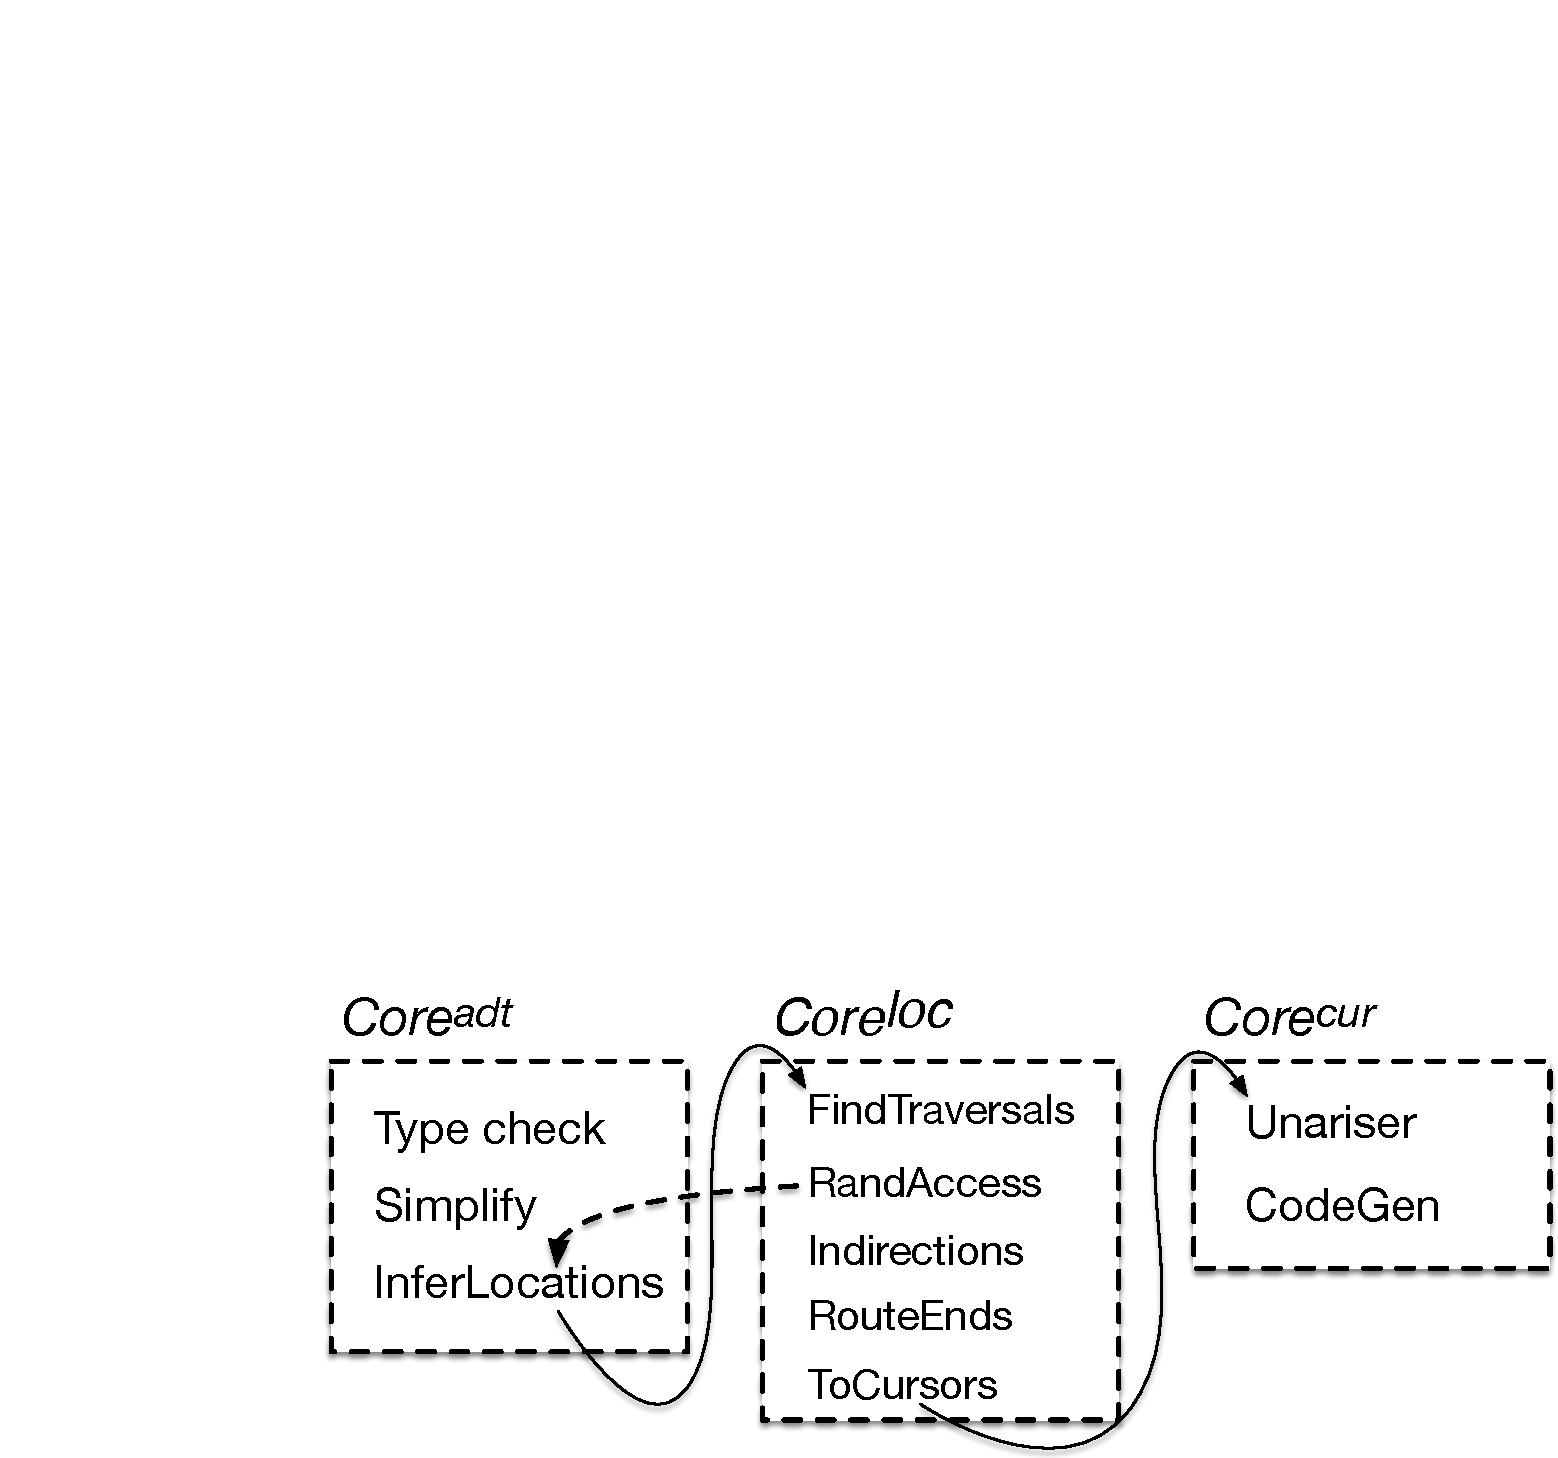
\includegraphics[width=0.6\textwidth]{compiler_arch}
  \caption{Compiler architecture.  Here we show the most important
    passes within the three phases of the compiler delimited by
    the three core IRs (front-end, middle-end, back-end).}
  \label{fig:compiler-arch}
\end{figure*}

\subsubsection{Finding Traversals}
\label{sec:find-traversal}

%% After location inference produces a valid \ourcalc{} program, the program is
%% still in a form that assumes access to any field of a data constructor.

%% In order to efficiently compile expressions with pattern matching on data
%% structures {with one or more fields which are not indirections}, the
%% compiler needs to generate code for computing the pointers of each field of the
%% structure in order to bind them to pattern variables.

Pattern matches in \ourcalc bind all constructor fields, including those that
occur at non-constant offsets, later in memory.
%
The compiler must determine which fields are reachable based on either (1)
constant offsets, (2) stored offsets/indirections present in the datatype, or
(3) by leveraging traversals already present in the code that scan past the
relevant data.
%
The third case corresponds to determining end witnesses in the formal semantics.
%% and in general \ourcalc{} allows for all fields in any
%% data structure to be bound by pattern matching.
%
%% That is, for a pattern match on \il{Node x y}, the program may assume that it
%% can reference \il{y} and therefore (implicitly) compute the end witness of \il{x} to reach
%% the address of \il{y} in memory.
%
% including those to the right of inline-serialized child structures.
Likewise, this compiler pass identifies data reached by the work the program
already performs.

%% %% we have an extremely simple metric for whether it is at risk of increased work
%% %% and degraded asymptotic complexity:
%% %% \begin{itemize}
%% %% \item Was a \il{copy} inserted?
%% %% \item Does the program refer to a location
%% %% \end{itemize}

%% %% After the location inference algorithm generates a \ourcalc{} program,
%% %% we run {a simple analysis to check if the asymptotic complexity of
%% %%   any of the functions has changed},
%% %% \rn{no that's not simple in general!}
%% %% and if it has, we add
%% %% layout information to the program to restore it.
%% %% Since the location inference algorithm applies some `known' program
%% %% repair strategies like inserting calls to copy functions,
%% %% adding dummy traversals etc. performing this analysis is a simple matter
%% %% identifying these repair strategies and
%% %% replacing them with more efficient ones.
%% %% All calls to copy functions can be eliminated just by inserting
%% %% an indirection node instead.
%% %% However, doing the same for traversal functions
%% %% is tricky and requires some further analysis.


To this end, we use a variation of a technique we previously proposed
\cite{ecoop17-gibbon}.  Specifically, we assign \emph{traversal effects} to
functions.  A function is said to {\em traverse} it's input location if it
touches every part of it.  In \ourcalc{}, a case expression is the only way to
induce a traversal effect.  If all clauses of the case expression in turn
traverse the packed elements of the corresponding data constructors, the
expression traverses to the end of the scrutinee.
%
Traversing a location means witnessing the size of the value encoded at that
location, and thus computing the address of the \emph{next} value in memory.
% (This is the $\phi$ function from \secref{sec:lang}).
%
After this pass, the type schemes of top-level function definitions reflect
their traversal effects.

%% This analysis is very similar to the \emph{effect inference} process
%% described in~\citet{ecoop17-gibbon}.
%% % , and we leave the reader to find more details in that paper.
%% The primary difference in our approach, other than the overall purpose (their
%% effect inference procedure is used to infer something like location annotations,
%% though ``abstract locations'' in that paper are quite different than what we
%% call locations---and, in fact, unnecessary traversals and copies are inserted
%% into Gibbon programs after effect inference), is that no unification is
%% required.

\begin{code}
maplike : forall $\locreg{l_1}{r_1}$ $\locreg{l_2}{r_2}$. @\tyatlocreg{Tree}{l_1}{r_1}@ $\xrightarrow{\{ l_1, l_2 \}}$ @\tyatlocreg{Tree}{l_2}{r_2}@
rightmost : forall $\locreg{l}{r}$ . @\tyatlocreg{Tree}{l}{r}@ $\xrightarrow{\{\}}$ Int
\end{code}

\subsubsection{Implementing Random Access}
\label{sec:rand-access}
% ~~~~~~~~~~~~~~~~~~~~~~~~~~~~~~~~~~~~~~~~
%% (by changing data constructors to contain random-access skip-ahead pointers, and
%% thus avoiding any need for dummy traversals in these situations).

Once we know what fields are traversed, we can also determine which fields are
used but \emph{not} naturally reachable by the program: e.g. the right subtree
read by \il{rightmost}.
%
% Compiled in the style of
% If we take no further action, \il{sizeof(left)}
In later stages of the compiler, we eliminate all direct references to
pattern-matched fields {\em after} the first variable-sized one.
%
This is where space/time optimization choices must be made:
bytes for offsets v.s. cycles for unnecessary traversals.

%% Through this compiler pass we determine which functions \emph{do not}
%% traverse their inputs, and hence if it is necessary to modify the
%% data structures those functions operate on to allow them to execute
%% efficiently.
%% For example, a function that returns the leftmost leaf of a tree does not
%% traverse its input, but it can be compiled without any modifications to use the
%% default serialization format.
%% %
%% Conversely, the \il{rightmost} function does not touch all input bytes, \emph{and}
%% needs additional support from the datatype to avoid asymptotically expensive
%% dummy traversals.
%% %
%% To avoid this, we enumerate all data-types where we need to ``skip over''
%% variable-sized fields and we modify the data type to enable random-access.

% \paragraph{Random-access nodes include offsets}
% \paragraph{Adding offsets}
%\paragraph{Layout Information}
\label{sec:RAN}
% ~~~~~~~~~~~~~~~~~~~~~~~~~~~~~~~~~~~~~~~~

%% When the compiler knows for sure that a data constructor being allocated will
%% need random access to its fields, it can do much better than implementing all
%% fields as \emph{tagged} indirection nodes.
%% First of all, random access to field $N$ would
%% require that \emph{all} fields $1 \ldots N-1$ be indirection nodes in order to
%% make assumptions about the offset to reach field $N$, which negates the
%% flexibility of tagged indirections occurring anywhere.
%% Second, the aforementioned space and time overheads for dispatching on
%% ``\il{I}'' tags would add up.

To activate random-access for a particular field within a data constructor, we
add additional information following the tag.  Specifically, for a constructor
\il{K T1 T2}, if we need immediate access to \il{T2}, we include a 4-byte
relative-offset after the constructor.
% \il{K' (Ptr T2) T1 T2}.
%
%% (We never do this for the leftmost field, which we can already reach in constant
%% time.)  
%% applying this technique to the running example datatype yields:
%% \begin{code}
%%   data Tree = Leaf Int | ${\color{blue} {\q{Node'}\ \q{(Ptr Tree) Tree Tree}}}$
%% \end{code}
%%
%% Here we have eliminated the original \il{Node} constructor, but we could also
%% keep both variants; in future work we plan to explore this possibility.
%% %
%% The random-access constructor \il{Node'} takes one word more space,
%% saving on space compared to a traditional pointer-based
%% representation\footnote{It may look like \il{Node'} has three fields, but at
%%   runtime this does not imply three words.  Rather, the naked \il{Tree} fields
%%   are still serialized directly in the stream, and so they are more akin to
%%   promises of future data on the stream, than fields in traditional structs or
%%   tuples.},
%% yet it can still be consumed either in-order or via random-access.
%% %
%% If reading \il{Tree} in-order, the reader ignores the \il{Ptr Tree} field and
%% reads the left- and right-subtrees as usual.
%% %
%% %% The random-access technique is composable with the indirection technique,
%% %% increasing the space of possible encodings (and we could mix and match normal
%% %% and random-access constructors within an encoding as well, \il{Node} and
%% %% \il{Node'}).
%% %
%% An example with random-access nodes is pictured below, including
%% relative offsets, and representing the source expression

%% \lstinline{Node (Node (Leaf 1) (Leaf 2)) (Node (Leaf 3) (Leaf 4))}.

%% %
%% \begin{center}
%%   \includegraphics[width=0.4\textwidth]{figs/tree_random_access_nodes}
%% \end{center}
%
%% Unlike tagged indirections, random-access nodes use fewer bytes than a
%% traditional pointer-based representation.  In this tree example, we use
%% \emph{one} word for pointer data, rather than two words (both left and right
%% pointers).  Compared with the tagged-indirection version, this saves a couple of
%% bytes on tags as well as the runtime overhead of switching on them.

%% % In total, this encoding takes 45 bytes rather than the 47 with tagged
%% % Overall, the left encoding above takes 29 bytes, and the right takes 47 bytes.

% \subsubsection{Back-tracking to add random-access}
\paragraph{Back-tracking}
%
Unfortunately, when we modify datatypes to add offsets, we invalidate
previously computed location information.  Thus the compiler {\em backtracks},
rewinding in time to before find-traversals (and inserting extra \il{letloc}
expressions to skip-over the offset bytes themselves).
% InferLocations
% (as pictured in \figref{fig:compiler-arch}), restoring correct location information.
%
Adding random access to one datatype never \emph{increases} the set of
constructors needing random-access to maintain work-efficiency, so in fact we
only backtrack at most once\footnote{The marked set of constructors
  is a conservative over-approximation; it would be possible in principle to
  construct a program with types \il{A} and \il{B}, both of which are marked for
  random access, but where \il{A} becoming random-access would obviate the need
  for \il{B}.  Further optimizations are possible.}.
%
%
After this is complete, the \il{rightmost} example becomes:
%
\begin{code}
rightmost : @\tyatlocreg{Tree}{l_{1}}{r_1}@ -> Int
rightmost tr =
 case tr of
   Leaf (n : @\tyatlocreg{Int}{l_n}{r_1}@ ) -> n
   Node' (ran : (Ptr (@\tyatlocreg{Tree}{l_b}{r_1}@)) @\tyatlocreg{}{l_{ran}}{r_1}@)
         (a : @\tyatlocreg{Tree}{l_a}{r_1}@) (b : @\tyatlocreg{Tree}{l_b}{r_1}@)
      -> rightmost [@\locreg{l_{b}}{r_1}@] *ran
\end{code}
\note{TODO: Clarify notation for using RAN pointers}
% \note{TOOD: Make the `read RAN and then call rightmost with it' step explicit in the example.}


%% That's because it never uses the right child of the tree, which it cannot reach
%% without a dummy traversal.  So we perform a simple occurs-check to look for uses
%% of such {\em unreachable} packed elements in the function body, and mark the
%% corresponding data constructor as needing random access if so.
%
In the default (offset-adding) mode, any function that demands random access to
a field will determine the representation for all functions using the
datatype.
%
Our current LoCal compiler does \emph{not} automate choices such as duplicating
datatypes to achieve multiple encodings of the same data---that is left to the
programmer or upstream tools.

If the LoCal compiler is passed a flag to {\em not} automatically change
datatypes, then it must use the same approach we previously used in~\cite{ecoop17-gibbon}:
insert {dummy traversals} that scan across earlier
fields to reach later ones.
%
Regardless of whether the offset or dummy-traversal strategy is used,
%
at the end of this compiler phase, we blank non-first fields in
each pattern match to ensure they are not referenced directly.
So a pattern match in our tree examples becomes
 ``\il{Node a _ -> ...}'' or   ``\il{Node offset a _ -> ...}''.
% with the location of the right child, $l_b$, computed by other means if needed.


%% \begin{code}
%%   Node' (ran : (Ptr (@\tyatlocreg{Tree}{l_b}{r_1}@)) @\tyatlocreg{l_{ran}}{r_1}@) (a : @\tyatlocreg{Tree}{l_a}{r_1}@) _ -> rightmost [@\locreg{l_b}{r_1}@] b
%% \end{code}

%% %% Depending on the result of the previous analysis, we switch the serialization format
%% %% include layout information.
%% %% This is a rather radical transformation, which affects all parts of the program.
%% %% An important thing to note is that \q{AddLayout} operates on \lamadt{} programs,
%% %% rather than \ourcalc{}.
%% %% Because once we include indirection nodes in the serialization,
%% %% the locations inferred in the previous phase are no longer valid.
%% %% For example, in the tree serialization shown in \figref{fig:tree-packed},
%% %% the left child is serialized immediately after the Node tag.
%% %% Whereas in \figref{fig:indirections-layout}, we have to skip over
%% %% the indirection node to get to the left child.
%% %% So we essentially `go back in time', update the serialization format, and then run
%% %% location inference again to ensure that the location arithmetic is valid.
%% %% In practice, \q{AddLayout} takes in a \lamadt{} program, transforms it to include indirection nodes,
%% %% and runs a few compiler passes again to get back a \ourcalc{} program.
%% %% %
%% %% \rn{Wait, is it just proper backtracking at this point? We can just draw a
%% %%   back-edge in the architecture diagram.}

%% %% Adding layout information involves the following steps:

%% %% \begin{enumerate}
%% %% \item In the current implementation, indirection nodes are encoded as
%% %%   constructors of regular packed datatypes.  So we first update the data
%% %%   types to have an additional constructor which takes in a pointer argument.
%% %% \begin{code}
%% %% data Tree = Leaf Int
%% %%           | Inner Tree Tree
%% %%           | ${\color{blue} {\q{Indirection}\ \q{Pointer}}}$
%% %% \end{code}

%% %% \item Update all data constructors having $n$ packed arguments, to accept
%% %%   additional $(n-1)$ arguments to store the indirections.

%% %% \begin{code}
%% %% data Tree = Leaf Int
%% %%           | Inner ${\color{blue} \q{Tree}}$ Tree Tree
%% %%           | Indirection Pointer
%% %% \end{code}
%% %% \end{enumerate}


%% Note that adding random-access to data-types involves changing the
%% data-constructors that construct those values and every case
%% expression that consumes them.  However, at this phase of the compiler
%% (\lamadt{} and \ourcalc), the skip-ahead pointers are {\em not} used by  the
%% operational semantics (and thus neither by an interpreter for the IR).
%% %
%% Rather, they are dormant until the conversion to the cursor-based \lamcur{} IR.
%% %
%% For instance, a data constructor application \il{Node x y}, becomes \il{Node
%%   (ptrEndOf x) x y} (using a compiler primitive \il{ptrEndOf}), and a case
%% expression matches the added pointer field, but ignores it  until later.

%% %% \begin{code}
%% %% case tree of Node $\color{blue} {(yp\ @\ {l_i} ^ {r})}$ (x $@\ {l_1} ^ {r}$) (_ $@\ {l_2} ^ {r}$) -> $\ldots$
%% %% \end{code}

%% % Update the constructor functions, (MkNode), to write the indirection nodes.

%% %% \begin{code}
%% %% addLayout : $\lamadt{}$ -> $\lamadt{}$
%% %% addLayout ex =
%% %%   case ex of
%% %%     DataConE con args ->
%% %% \end{code}

\subsubsection{Routing End Witnesses}
\label{sec:route-ends}
% \subsection{Route-Ends, To-Cursors, and Code Generation}
% ~~~~~~~~~~~~~~~~~~~~~~~~~~~~~~~~~~~~~~~~

%% Gibbon, as described in~\citep{ecoop17-gibbon}, transforms a
%% functional program operating on algebraic data structures using
%% pattern matching into a pointer-passing (or ``cursor''-passing)
%% imperative program.
%% %
%% Our compiler also must do a similar transformation, though unlike in
%% \citet{ecoop17-gibbon}, \ourcalc{} enables these steps in our compiler to be

Each of the traversal effects previously inferred proves we logically reach a
point in memory, but to realize it in the program we add an
additional return value to the function, witnessing the end-location for
traversed values (as described in \cite{ecoop17-gibbon}).
%
We extend the syntax to allow additional location-return values,
equivalent to returning tuples.  The \il{buildtree} example becomes:
%

\begin{code}
buildtree : forall $l^r$. Int $\xrightarrow{\{l\}}$ [$\mathit{after}(\tyatlocreg{Tree}{l}{r})$] Tree$\locreg{@l}{r}$
buildtree [$\locreg{l}{r}$]  n =
  if n == 0 then return [$\locreg{l}{r}+9$] (Leaf $\locreg{l}{r}$ 1)
  else letloc $\locreg{l_a}{r}$ = $\locreg{l}{r}$ + 1 in
       let [$\locreg{l_b}{r}$] left = buildtree [$\locreg{l_a}{r}$] (n - 1) in
       let [$\locreg{l_c}{r}$] right = buildtree [$\locreg{l_b}{r}$] (n - 1) in
       return [$\locreg{l_c}{r}$] (Node $\locreg{l}{r}$ left right)
\end{code}% \vspace{-1mm}
%% letloc $l_{ran}$ = $l_1$ + 1 in
%% letloc $l_a$ = $l_{ran}$ + 8 in
%                @{let ran = (ptr) $l_b$ in}@

%% Above, the use of \il{after} has disappeared.  With
%% the additional end-witnesses returned by the recursive calls, the previous
%% \il{sizeof} was not needed to compute $l_b$, and thus it was dropped as dead
%% code.

The \il{letloc} form for the location of the right subtree is gone, because
the first recursive call to \il{buildtree} returned $\locreg{l_b}{r}$ as an end-witness,
bound here with an extended \il{let} form.
Similarly, the final return statement returns the end-witness of the right subtree,
$\locreg{l_c}{r}$, using a new \il{return} form in the IR.

\subsubsection{Converting to \lamcur}
% ~~~~~~~~~~~~~~~~~~~~~~~~~~~~~~~~~~~~~~~~
\label{sec:cursorize}

In this stage, we convert from \ourcalc{} into \lamcur{}, switching to
imperative cursor manipulation.
%
%% Unlike previous published techniques,
%% \ourcalc{} makes this step entirely type-directed and relatively
%% straightforward.
%% %
%% % \item \textbf{To-Cursors}:
%% %% Each function is further transformed to remove normal function argument bindings
%% %% and pattern-match variable bindings. The threaded-through locations from the
%% %% previous step become \emph{cursors}, and the program works imperatively on these
%% %% cursors.
%% %
%% %% {Cursorize}
%% %% \note{Probably has too much in common with the ECOOP17 paper.}
At this stage, location arguments and return values turn into first-class cursor
values (pointers into memory buffers representing regions).  The primitive
operations on cursors read or write one atomic value, and advance the cursor to
the next spot.  We drop much of the type information at this phase, and
\il{rightmost} becomes:
\begin{code}
rightmost : Cursor -> Int
rightmost cin =   -- take a pointer as input 
  switch cin of   -- read one byte
    Leaf(cin1)  -> 
      let (cin2,n) = readInt(cin1) in n
    Node(cin1)  -> -- only get a pointer to the 1st field
      let (cin2,ran) = readCursor(cin1) in
      rightmost ran
\end{code}\vspace{-1mm}
%
Here the \il{switch} construct is simpler than \il{case},
% is no longer pattern matching on data constructors to access fields, rather it is
reading a one byte tag, switching on
it, and binding a cursor to the very next byte in the stream
(\il{cin1 == cin + sizeof(tag) == cin+1}).

%
The key takeaway here is that, because the relationship between
location variables and normal variables representing packed data are
made explicit in the types and syntax of \ourcalc{}, this pass
does not require any complicated analysis.
%
Also, in \lamcur{} we can finally reorder writes to more often be {\em in order}
in memory, which aids prefetching and caching,
%\footnote{Linear access patterns are more friendly to prefetching \&
%  caching policies in modern processors.},
because writes are ordered only by
data-dependencies for computing \emph{locations}, with no ordering needed
on the side-effects themselves.





\chapter{Applications and Evaluation}
\label{chapter:applications}
\note{General overview of the kinds of things we tested in Gibbon, how fast they were, etc.}

\section{Microbenchmarks}

See \tabref{tab:litmus-table}.

We are
% gibbon pointer cnf capn
202 / 2.6 / 3.2 / 9.4  $\times$ geomean faster than
Gibbon/NonPacked/CNF/CapNP respectively, and
0.96 / 2.6 / 3.2 / 7.3 $\times$ faster for only apples-to-apples asymptotics.
%% $3.2\times$,
%% $9.4\times$, and
%% $202\times$


%% \tabref{tab:litmus-table} shows the results.

\note{Re-write to either remove or better explain difference between Gibbon1 and Gibbon2.}
      
The column labeled ``Gibbon2'' shows performance of \lamadt programs
(low-level \ourcalc control was not needed for any of these)
using indirections and offsets, automatically.
%
``Gibbon1'' shows the approach described in \cite{ecoop17-gibbon}.
%
There are two major sources of overhead for our new approach versus Gibbon1:
 
\begin{enumerate}
\item Growable regions:
In each case, our compiler starts with smaller, growable regions\footnote{starting at 64K bytes}, 
which we require to create small output regions as
in {\bf id} or {\bf treeInsert},
but we suffer the overhead of bounds-checking. On the other hand,
Gibbon always stores fully serialized data in huge regions.

\item Likewise, we have found that the backend C compiler is sensitive to the number
of cases in switch statements on data constructor tags (for instance, triggering
the jump table heuristic).  By including the possibility that each tag we read
may be a tagged indirection,
% or end-of-chunk,
we increase
code size and increase the number of cases in our switch statements.
\end{enumerate}


However, the benchmarks where indirections and random-access offsets are important (id,
rightmost, treeInsert, findMax) show a huge difference between Gibbon1 and Gibbon2,
as we would expect based on Gibbon1
requiring additional traversals to compile those functions.

\paragraph{Versus pointer-based representations}
The ``NonPacked'' approach is \ourcalc configured to always insert indirections
and thus emulate a traditional object representation.
% example of a traditional compilation approach
% that use one heap object per data constructor.
%
In this case, we are being overly friendly to this pointer-based representation by
allowing it to read its input (for example, the input tree to {\bf treeInsert})
in an already-deserialized, pointer-based form.  A full apples-to-apples
comparison would force the pointer-based version to deserialize the input
message and reserialize the output; but we omit that here to focus only on the
cost of the tree traversals themselves.
%
%% Similarly, the earlier Gibbon work compared a subset of these programs against a
%% larger set of traditional compilers (Java, gcc, GHC, OCaml, MLton, Racket, Chez),
%% finding those compilers performance on
%% pointer-based inputs worse than the performance of lifted functions on
%% serialized inputs.

\paragraph{Versus competing libraries}

%% The CNF representation is just the traditional Haskell heap representation of
%% data constructors.  It wastes a word of header space for garbage collection
%% purposes, and it uses full 64-bit absolute pointers between heap objects.
%% The result is fast to read but not space efficient.
%% This is visible on benchmarks such as {\bf sumTree}, where CNF out-performs
%% Cap'N Proto by $3.5\times$.
%% % (/ 0.96 0.27)
%% Conversely, the Cap'N Proto representation is space efficient---using 40\% fewer
%% bytes for the binary tree---and faster to build.
%% % (- 1 (/ 805 1340.0))
%% %
%% CNF results are slow to build because they involve an extra copy: first to
%% create the data on the normal heap, second to copy it into the compact region.
%% This is why CNF's {\bf copyTree} is twice as fast as {\bf add1Leaves}, even
%% though the both computations walk the tree and build a new output tree, copy is
%% able to use a runtime system function to walk the data and copy directly from
%% input message to output message, without allocating on the regular (non-compact)
%% Haskell heap.

The biggest differences in \tabref{tab:litmus-table} are due
asymptotic complexity.
However, for constant factor performance, we see the expected
relationship---that our approach and Gibbon are faster than CNF and Cap'N Proto,
sometimes by an order of magnitude, \eg\,{\bf add1Leaves}.

CNF and Cap'N Proto encode some metadata in their serialization, to
support the GHC runtime, and protocol evolution, respectively.
On the other hand, 
our compiler only uses offsets and tagged indirections
when needed, and the size ratio of the encodings depends on how much these features are used.
%
For example, {\bf rightmost} uses a data-encoding that includes random-access
offsets, and {\bf treeInsert} creates an output with a logarithmic number of
tagged indirections.  Thus while our size advantage over CNF is
%
$4\times$ smaller
% (/ 1340.0 335)
%
on {\bf buildTree}, it is only
%
$2.22\times$
% (/ 1340.0 603)
% (/ 1340000000.0 (+ 334000000 (* (- (expt 2 25) 1) 8)))
%
for {\bf rightmost}.
% , and $XYZ\times$ for {\bf treeInsert}.

CNF results are slow to build because they involve an extra copy: first to
create the data on the normal heap, second to copy it into the compact region.
This is why CNF's {\bf copyTree} is twice as fast as {\bf add1Leaves}, even
though the both computations walk the tree and build a new output tree, copy is
able to use a runtime system function to walk the data and copy directly from
input message to output message, without allocating on the regular (non-compact)
Haskell heap.

\paragraph{Composing traversals}

For offset-insertion, we allow the whole-program compiler to select the data
representation based on what consuming functions are applied to it.
%% In a more general setting (say, modular compilation, or messages received over
%% the network from program in another language), we would need to adopt
%% random-access nodes uniformly, which would, e.g., give {\bf leftmost} the same
%% small amount of overhead in its input tree as {\bf rightmost}.
In the presence of multiple functions traversing a single data structure,
any function demanding random access changes the representation for all of them.
% the ``weakest link'' determines how many random-access nodes are needed.
% compiler uses a data representation required to optimize the slowest one.
{\bf repMax} is one such example:
%\begin{code}[mathescape=true]
\il{ repMax t = propagateConst (findMax t) t}.
%\end{code} \vspace{-5mm}
%  repMax = propagateConst . findMax -- almost correct!
% Consider the {\bf repMax} program in which
Here {\bf findMax} only requires a partial scan (random access), but propagating
that value requires a full traversal.  In this case, the compiler would add
offsets to the datatype to ensure that `findMax' remains
logarithmic.
%
However, this causes the subsequent traversal (propagateConst) to slow
down, as it now has to unnecessarily skip over some extra bytes.  Likewise, if
we do not include findMax in the whole program, the data remains fully
serialized, which is why {\bf propagateConst} and {\bf findMax} run separately
take less than 440ms, but run together take 480ms.  Yet the latter time is still
6$\times$ and 9$\times$ faster, respectively, than CNF and Cap'N Proto!
      


 \begin{table*}
  \begin{center}
    \small
      \begin{tabular}{ |c|c|c|c|c|c| }
        \hline
        Benchmark & Gibbon2 & Gibbon1 & NonPacked & CNF & CapnProto\hspace{-1mm} \\
        \hline
        % CNF: 100M iterations, calling NOINLINE id' function from NOINLINE rep.
        %      That gives 8.0ns (Allowing rep to inline, but not ID, makes it 2.15ns)
        % capnp: iter=20M median of 9 trials
        % Gibbon2: 100M iterations

        % Speedup:
        % CNF: (/ 2.1 2.1) = 1
        % CapnProto: (/ 129 2.1) = 61.42
        % Gibbon1: 152380952
        % Pointer: (/ 0.93 2.1) = 0.44
        {\bf id}:
        time, & 2.1ns &  0.32s  &  0.93ns &  2.1ns   & 129ns  \\
        complexity   & $O(1)$   &  $O(N)$ & $O(1)$    &  $O(1)$  & $O(1)$  \\
        %  output size (bytes)  &        &         &           &  8       &   8     \\
        \hline

        % CNF: 100M
        % capnp: iters = 20M median of 9

        % Speedup:
        % CNF: (/ 44 17.0) = 2.58
        % CapnProto: (/ 376 17.0) = 22.11
        % Gibbon1: (/ 18.0 17.0) = 1.05
        % Pointer: (/ 26 17.0) = 1.52
        {\bf leftmost}:
        time,        & 17ns         & 18ns        & 26ns        &    44ns      & 376ns            \\
        complexity   & $O(log(N))$  & $O(log(N))$ & $O(log(N))$ & $O(log(N))$  & $O(log(N))$ \\
        input size (bytes) & 335MB  & 335MB       & 335MB       &    1.34GB    & 805MB             \\
        \hline

        % CNF: 100M iterations
        % capnpL iter=20M, median of 9 trials
        % capnpL iter=20M, median of 9 trials
        % Speedup:
        % CNF: (/ 47 175.0) = 0.26
        % CapnProto: (/ 482 175.0) = 2.75
        % Gibbon1: 297142
        % Pointer: (/ 19 175.0) = 0.108
        {\bf rightmost}:
        time,        & 175ns        & 56ms    & 19ns        &    47ns      & 482ns \\
        complexity   & $O(log(N))$  & $O(N)$  & $O(log(N))$ & $O(log(N))$  & $O(log(N))$  \\
        input size (bytes) & 603MB & 335MB    & 335MB       &    1.34GB    & 805MB            \\
        \hline

        %capn: median of 9 trails iter=1
        % Speedup
        % CNF: (/ 4.5 0.27) = 16.66
        % CapnProto: (/ 1.8 0.27) = 6.66
        % Gibbon1: (/ 0.24 0.27) = 0.88
        % Pointer: (/ 2.7 0.27) = 10
        {\bf buildTree}:
        time,               & 0.27s     &  0.24s    & 2.7s &  4.5s  & 1.8s   \\
        complexity,         & $O(N)$    &  $O(N)$   &  $O(N)$ & $O(N)$  &  $O(N)$ \\
        output size (bytes) & 335MB     &  335MB    &  1.34GB &  1.34GB &  805MB       \\
        \hline

        % CNF: median of 9 trials:
        % capnp: median of 9 trails iter=1
        % Speedup:
        % CapnProto: (/ 3.8 0.25) = 15.2
        % CNF: (/ 2.7 0.25) = 10.8
        % Gibbon1: (/ 0.24 0.25) = 0.96
        % Pointer: (/ 3.1 0.25) = 12.4
        {\bf add1Leaves}:
        time,               & 0.25s     &  0.24s  & 3.1s     & 2.7s    &  3.8s  \\
        complexity,         & $O(N)$    &  $O(N)$ & $O(N)$   & $O(N)$  &  $O(N)$ \\
        \hline
        % CNF: median of 9 trials:
        % capn: median of 9 trails iter=1
        % Speedup:
        % CNF: (/ 0.27 0.095) = 2.84
        % CapnProto: (/ 0.96 0.095) = 10.10
        % Gibbon1: (/ 67.0 95) = 0.70
        % Pointer: 8.5
            {\bf sumTree}:
            time,               & 95ms     & 67ms     & 0.81s   &  0.27s  &  0.96s  \\
            complexity,         & $O(N)$   & $O(N)$   & $O(N)$  & $O(N)$  &  $O(N)$ \\
            \hline
            %capn: median of 9 trials iter =1
            % Speedup:
            % CNF: (/ 1.1 0.2) = 5.5
            % CapnProto: (/ 1.9 0.2) = 9.4
            % Gibbon1: (/ 0.24 0.2) = 1.2
            % pointer: (/ 3.5 0.2) = 17.5
                {\bf copyTree}:

                time,               & 0.2s      & 0.24s   & 3.5s   &  1.1s   &  1.9s       \\
                complexity,         & $O(N)$    & $O(N)$  & $O(N)$ & $O(N)$  &  $O(N)$ \\

                \hline
                \hline
                % CNF: median of 9 iters
                %capn: median of 9 trils iter=1
                % Gibbon numbers: median of 9 trials
                % Speedup:
                % CNF: (/ 4.27 0.5) = 8.54
                % CapnProto: (/ 2.1 0.5) = 4.2
                % Gibbon1: (/ 0.49 0.5) = 0.98
                % Pointer: (/ 2.96 0.5) = 5.92
                    {\bf buildSearchTree}:

                                    & 0.5s      & 0.49s     & 2.96s   &  4.27s   &  2.1s         \\
                    complexity,          & $O(N)$    & $O(N)$    & $O(N)$  & $O(N)$   &  $O(N)$ \\
                    output size (bytes)  & 603MB     & 603MB     & 1.61GB  &  1.61GB  &  805MB      \\

                    \hline

                    % CNF iters=1M
                    % This one is 2.5us with iters=1000
                    %            1.24us with iters=200K
                    %            1.04us with iters=1M
                    % NonPacked iters=1M
                    %
                    % capnp iters=20M median of 9
                    % Speedup:
                    % CNF: (/ 1 0.69) = 1.44
                    % CapnProto: (/ 1.3 0.69) = 1.88
                    % Gibbon: 144927
                    % Pointer: (/ 0.92 0.69) = 1.33
                    {\bf treeContains}:
                    time,                & 0.69$\mu$s   & 0.1s  & 0.92$\mu$s  &  1$\mu$s    & 1.3$\mu$s \\
                    complexity,          & $O(log(N))$ & $O(N)$ & $O(log(N))$ & $O(log(N))$ & $O(log(N))$ \\
                    \hline

                    % CNF iters=200K
                    % Capn median of 9 , iter=1
                    % Gibbon2 iters = 3500000
                    % Speedup:
                    % CNF: (/ 3.5 0.87) = 4.02
                    % CapnProto: (/ 150 0.87) = 172.4
                    % Gibbon: 436781
                    % Pointer: (/ 2.5 0.87) = 2.87
                    {\bf treeInsert}:

                    time,                & 0.87$\mu$s  & 0.38s  & 2.5$\mu$s   &  3.5$\mu$s   &  150$\mu$s  \\
                    complexity,          & $O(log(N))$ & $O(N)$ & $O(log(N))$ & $O(log(N))$  & $O(N)$  \\
                    avg bytes added      & 677 bytes        &  603MB  & 856 bytes   &  848 bytes  & 805MB  \\
                    \hline

                    %capnp: median of 9 trails iters=1M
                    {\bf InsertDestructive}:
                                         &  NA   & NA   & NA   & NA  &  1.37$\mu$s       \\
                    complexity,          &       &      &      &     & $O(log(N))$ \\

                    \hline

                    % Gibbon2:   100M iters
                    % Gibbon1:   20 iters
                    % Pointer:   100M iters
                    % CNF:       100M iters
                    % CapnProto: 1M iters
                    % Speedup:
                    % CNF: (/ 75 206.0) = 0.36
                    % CapnProto: (/ 597 206.0) = 2.89
                    % Gibbon: 427184
                    % Pointer: (/ 41 206.0) = 0.199
                    {\bf findMax}:
                    time,                & 206ns        & 88ms    & 41ns        & 75ns         & 597ns        \\
                    complexity           & $O(log(N))$  & $O(N)$  & $O(log(N))$ & $O(log(N))$  & $O(log(N))$  \\
                    \hline

                    % Speedup:
                    % CNF: (/ 4.2 0.43) = 9.76
                    % CapnProto: (/ 2.8 0.43) = 6.51
                    % Gibbon: (/ 0.42 0.43) = 0.97
                    % Pointer: (/ 3.3 0.43) = 7.67
                    {\bf propagateConst}:
                                         & 0.43s  &  0.42s  &  3.3s   & 4.2s   & 2.8s   \\
                    complexity,          & $O(N)$ &  $O(N)$ &  $O(N)$ & $O(N)$ & $O(N)$  \\
                    \hline

                    % Speedup:
                    % CNF: (/ 4.3 0.48) = 8.9
                    % CapnProto: (/ 2.9 0.48) = 6.04
                    % Gibbon: (/ 0.51 0.48) = 1.06
                    % Pointer: (/ 3.2 0.48) = 6.67
                    {\bf repMax}:
                    time,                & 0.48s  & 0.51s   & 3.2s    & 4.3s    & 2.9s   \\
                    complexity,          & $O(N)$ & $O(N)$  & $O(N)$  & $O(N)$  & $O(N)$  \\

                    \hline
      \end{tabular}
    \end{center}
  \vspace{-3mm}
    \caption{Tree-processing functions operating on serialized data.
      %% We are
      %% % gibbon pointer cnf capn
      %% 202 / 2.6 / 3.2 / 9.4  $\times$ geomean faster than
      %% Gibbon/NonPacked/CNF/CapNP, and
      %% 0.96 / 2.6 / 3.2 / 7.3 $\times$ faster for only apples-to-apples asymptotics.
      %% %% $3.2\times$,
      %% %% $9.4\times$, and
      %% %% $202\times$
      %% \captionscrunch{}
    }
    \label{tab:litmus-table}

\end{table*}


\section{Data Processing Benchmarks}

\note{Overview of how this technique can be applied to data processing programs.}
\note{If data to be processed is already serialized then this avoids marshaling cost.}
\note{If data to be processed is in some other format then we can still be faster by
  transforming the data into a format that is more efficient to process (like the JSON
  to byte array transformation necessary for the Twitter benchmark). And in these cases
  it is often still faster than libraries that are meant to process the data in its
  original form.}
 

\subsection{Twitter JSON Benchmark}

For a real data set, we
use Twitter metadata consisting of user ID's and hashtags for all tweets posted
in 1 month, and count the occurrences of the hashtag ``cats'' in this dataset.
Here we seek to replicate and extend the CNF experiment reported by
\cite{cnf-icfp15}.

The dataset is stored on disk in JSON format, and we use RapidJSON
v1.1.0 ({\footnotesize\url{http://rapidjson.org/}}) as a performance baseline: a widely
recognized fast C++ JSON library.
%
In \figref{fig:twitter_slowdown_plot}, we vary the amount of data processed,
up to 1GB.  (For each data-point, taking the median of 9 trials
ensures the data is already in the Linux disk cache.)
%
For fairness, all versions read the data via a single \il{mmap} call, plus
demand paging.

There are two RapidJSON versions. The ``lexer'' version never constructs an
object representing a parsed tweet, rather, it is a state-machine
that is able to count ``cats'' while tokenizing, {\em without parsing}.  It is
optimized to be as fast as possible for this particular JSON schema, with no
error detection (a non-compliant input would give silent failures and wrong
answers).
%
The ``parser'' version represents a more traditional and idiomatic situation use
of the library: calling the \il{.Parse()} method to produce a DOM object, and
then accessing its fields.
%
We have structured this benchmark to maximally advantage this parsing approach:
the 9,111,741 tweets processed in the rightmost data points of \figref{fig:twitter_slowdown_plot} are stored as one JSON object each, on each line of the input file.
%
Thus the data only needs to be read into memory once, and in a single pass the RapidJSON benchmark reads, parses, discards, and repeats.
%
Conversely, if the tweets were instead stored as a single JSON array, filling
the entire input file, then RapidJSON would have to parse the entire file
(writing the DOM tree out to memory, overflowing last level cache), then read
that same tree back into memory in a second pass to count hashtags.
%
Nevertheless, in spite of this single-pass advantage, our compiler achieves
6$\times$ and 12$\times$ speedup over RapidJSON lexer/parser.
%
We process the 9.1M tweets in 0.39s.


\begin{figure}
  \centering
  \input{twitter_slowdown_plot}
  \caption{Twitter data processing benchmark results}
  \label{fig:twitter_slowdown_plot}
\end{figure}

\subsection{Point Correlation}

\note{Summarize Laith's point correlation benchmark (from ECOOP
  paper), updating the language to match the new terminology from
  LoCal.}
Point correlation  is a well-known algorithm used in data mining~\cite{gray2000n}:
given a set of points in a k-dimensional space, point correlation computes the number of points in that space  that lie within a
distance $r$ from a given point $p$. 

% Rather than comparing each point in the space to the query point, one efficient way of searching such spaces is to store them in kd-trees~\cite{bentley75}. KD-trees are space-partitioning trees where the root of the kd tree represents the entire space, and each node's children represents a partition of that node's space into two subspaces.

% A kd-tree is a binary space-partitioning tree that in its simplest form  splits the space at each internal node into two sub-spaces
% around a split axes in one of the space dimensions, the left subtree stores the points to the left of the split access
% and the right subtree sotres the points to the right of the split access, the split axes alternates between the dimensions of
% the space at each level of the tree, when the number of the points in the subtree is one, a leaf node that stores
% that point is constructed.


In a naive implementation of point correlation, each point in the space needs
to be checked against the query point. 
A more efficient approach is to use kd-trees~\cite{bentley75} to store the
points. KD-trees are space-partitioning trees where the root of the kd tree represents the entire space, and each node's children represents a partition of that node's space into two subspaces.
KD-trees allow the search
process to skip some regions in the space. By storing at each internal node
the boundaries within which all descendent points lies, the search process can
skip a subtree is a given point is far enough from the boundaries. As a
result, querying a kd-tree to perform point-correlation is $O(log\; n)$ instead
of $O(n)$. Note that it is exactly the process of ``skipping'' subtrees that
gives kd-tree-based point correlation its efficiency, but also that prevents a
normal packed representation from sufficing to implement the algorithm: there
is no way to skip past a subtree without performing a dummy traversal,
obviating the asymptotic performance gains.

We implemented both a standard pointer-based version of 2-point correlation in
C, as well as a version that operates over a packed representation augmented
with indirection pointers. Each interior node stores a rope-style
indirection pointer that maintains the size of its child subtrees. If a
traversal is truncated at that node, the cursor is incremented by the value in
that indirection pointer, skipping the subtrees and resuming traversal on the
rest of the tree.

\figref{fig:point_corr_plot} shows the speedup of the packed version
with respect to the standard pointer-based implementation for
different tree sizes. For each tree size, we ran 10 query points
through the tree. For small trees, the queries were performed 10000
times to produce sufficient runtime for accurate measurements. Each
experiment was performed 10 times, and the mean is reported.

For every tree size, the packed representation uses 56\% less memory
than the pointer-based trees. This reduction in memory usage has two
sources: nodes do not need to store left-child pointers; and more
efficient packing of data in the packed representation. For small
trees, the runtime performance of the packed and pointer versions are
comparable. For large trees, the packed version is up to 35\% faster
than the pointer-based version. 

The relatively smaller performance improvement for this
benchmark versus the Twitter benchmarks is unsurprising. First, taking an
indirection means that any spatial locality gains from the packed
representation are lost, resulting in similar behavior to the
pointer-based version. Second, there is relatively more work to be
done per node in this benchmark, so the time spent in traversal of the
tree is relatively less, reducing the opportunity for improvement.


\begin{figure}
  \centering
  \input{point_corr_plot}
  \label{fig:point_corr_plot}
  \caption{Speedup of serialized implementation of point correlation versus
    pointer-based implementation.}
\end{figure}

\section{Abstract Syntax Trees}

\note{This is where my results for ASTs will eventually go.}
\note{I can maybe put the Racket count nodes benchmark in here too, as a kind of
  AST traversal.}



%% \newpage

% \appendix command is necessary to change chapter numbering.
% Appendices are optional

\appendix

\chapter{\ourcalc Runtime System Details}
\label{chapter:rts}
% ================================================================================

In \ourcalc, locations track natural number positions within a region.
Abstractly, a region is an unbounded, byte-indexed storage area that can be
extended incrementally by requesting $N$ additional bytes (equivalent to
\il{malloc(N)}).
%
Each region grows monotonically, never shrinks, and can be
freed only as a whole.
%
Practically speaking, there are at many reasonable implementation strategies.
%
We always start by allocating a contiguous {\em chunk} of memory of bounded
size.  When that chunk is exhausted, we must choose whether to grow the
region by {\bf copying} (or changing memory-mapping), retaining a contiguous
address range, or by linking a new, non-contiguous chunk.


%% \begin{enumerate}
%% \item constant regions
%% \item unbounded regions: must grow to accommodate allocation.
%% \item huge regions: semantically the same as unbounded, but suspected to be very
%%       large and long-lived.
%% \end{enumerate}

We choose the latter and implement regions as a linked list of chunks: a
constant sized initial chunk, with subsequent chunks doubling in size.
%
% A reference to a region is just a pointer to its first chunk.
The runtime representation of locations (and \il{Ptr T} values)
is a direct pointer into the interior of a chunk.
(We call the writable portion of the chunk that can carry data the {\em payload}.)
Chunks linked together form regions as pictured in
\figref{fig:regions}.  Chunk metadata is stored at the \emph{end} of the
allocated area, in a footer data structure listed below:
%
\begin{lstlisting}[language=C++]
  struct footer {
    // Available bytes for serialized-data storage.
    int  size;
    // Shared reference count for this region (not chunk)
    int* refcount;
    // Set of regions we have outbound pointers into.
    ptrset  outset;
    // The chunk that follows this one (or NULL)
    footer* next;
  }
\end{lstlisting}
We avoid additional indirection by combining this metadata struct with the
payload, which is essentially an array of bytes, forming one heap object.
% \paragraph{Bounds-checking}
The reason we store the metadata as a \emph{footer}, at the end rather than the
start, is so that the payload grows \emph{towards} the struct.  Thus the pointer
to the region-chunk does double duty for bounds checking.  When the payload
space is full, we allocate a new chunk of double the size and point to it with
\il{next}.

But what do we put in the serialized bytestream to mark that the stream
continues in another chunk?  Here we implicitly add a reserved tag to each
packed data type, signaling {\em end of chunk} (EOC).\footnote{Of course, there
  are 256 possible one-byte tags, so adding indirections, random-access nodes,
  and EOC tags reduces the largest sum type supported (at least, without using
  an escape sequence to access additional tags).}
%
When the reader hits an EOC, they must use their pointer to the end of the
current payload to access the footer, follow the \il{next} pointer, and resume
reading at the head of the next chunk.

%% Here we introduce a slight variation on the concept
%% of an indirection node from \secref{sec:indirections}, a {\bf redirection
%%   node}.  When a consumer reads an \il{Indirection (Ptr T)} value from the
%% stream, it refers to the pointer to read a complete value of type \il{T} from
%% a distant address, but then it comes back to the original buffer, containing the
%% indirection, and continues.  In contrast,


\paragraph{Garbage collection}
% ~~~~~~~~~~~~~~~~~~~~~~~~~~~~~~~~~~~~~~~~

In most classic treatments, regions introduced with a \il{letregion},
are deallocated immediately upon the end of that \il{letregion}'s lexical
scope.
%
However, in this paper we choose to allow tagged indirection nodes to include
{\bf inter-region pointers}.  Thus one can keep a region alive beyond the scope of the
\il{letregion} that introduced it, by simply capturing a pointer to it within
another region.
%
This choice is critical to our ability to lift functions onto (mostly)
serialized representations without changing their asymptotic complexity.

In our setting, pointers between regions are immutable, which simplifies the job of
garbage collection.  Rather than keeping a ``remembered set'' of inter-region pointers as
in a generational collector, we can instead \emph{coarsen} the dependencies to record only
that ``chunk A points to region B''.  The \il{outset} in the \il{footer} struct above
tracks regions to which our chunk points\footnote{This set is optimized for zero or one
  elements.  A null pointer denotes the empty set, and singleton is a direct (tagged)
  pointer to the element.  Two or more elements introduce a heap data structure to store
  the out-set.}.

Both tracing or reference counting collectors would benefit from this
coarsening.  However, given that we already amortize the overheads of memory
management through coarsening, we choose reference counting for our
implementation to achieve prompt deallocation (and reuse) of chunks.
%
Thus when a region is created with \il{letregion} its reference count is set to 1,
and it is decremented on exit from the \il{letregion}.
%
Reference counts are region-level rather than chunk-level, which is why the
\il{footer} contains a pointer to the region-level reference count, rather than
a reference count directly.
%
When a region hits zero reference count, it is freed immediately via freeing its
chunks one by one.  When a chunk is deallocated, it decrements the reference
count of any regions it points to.


\floatstyle{plain}\restylefloat{figure}
\begin{figure}
  \vspace{-15mm}
  \begin{center}
    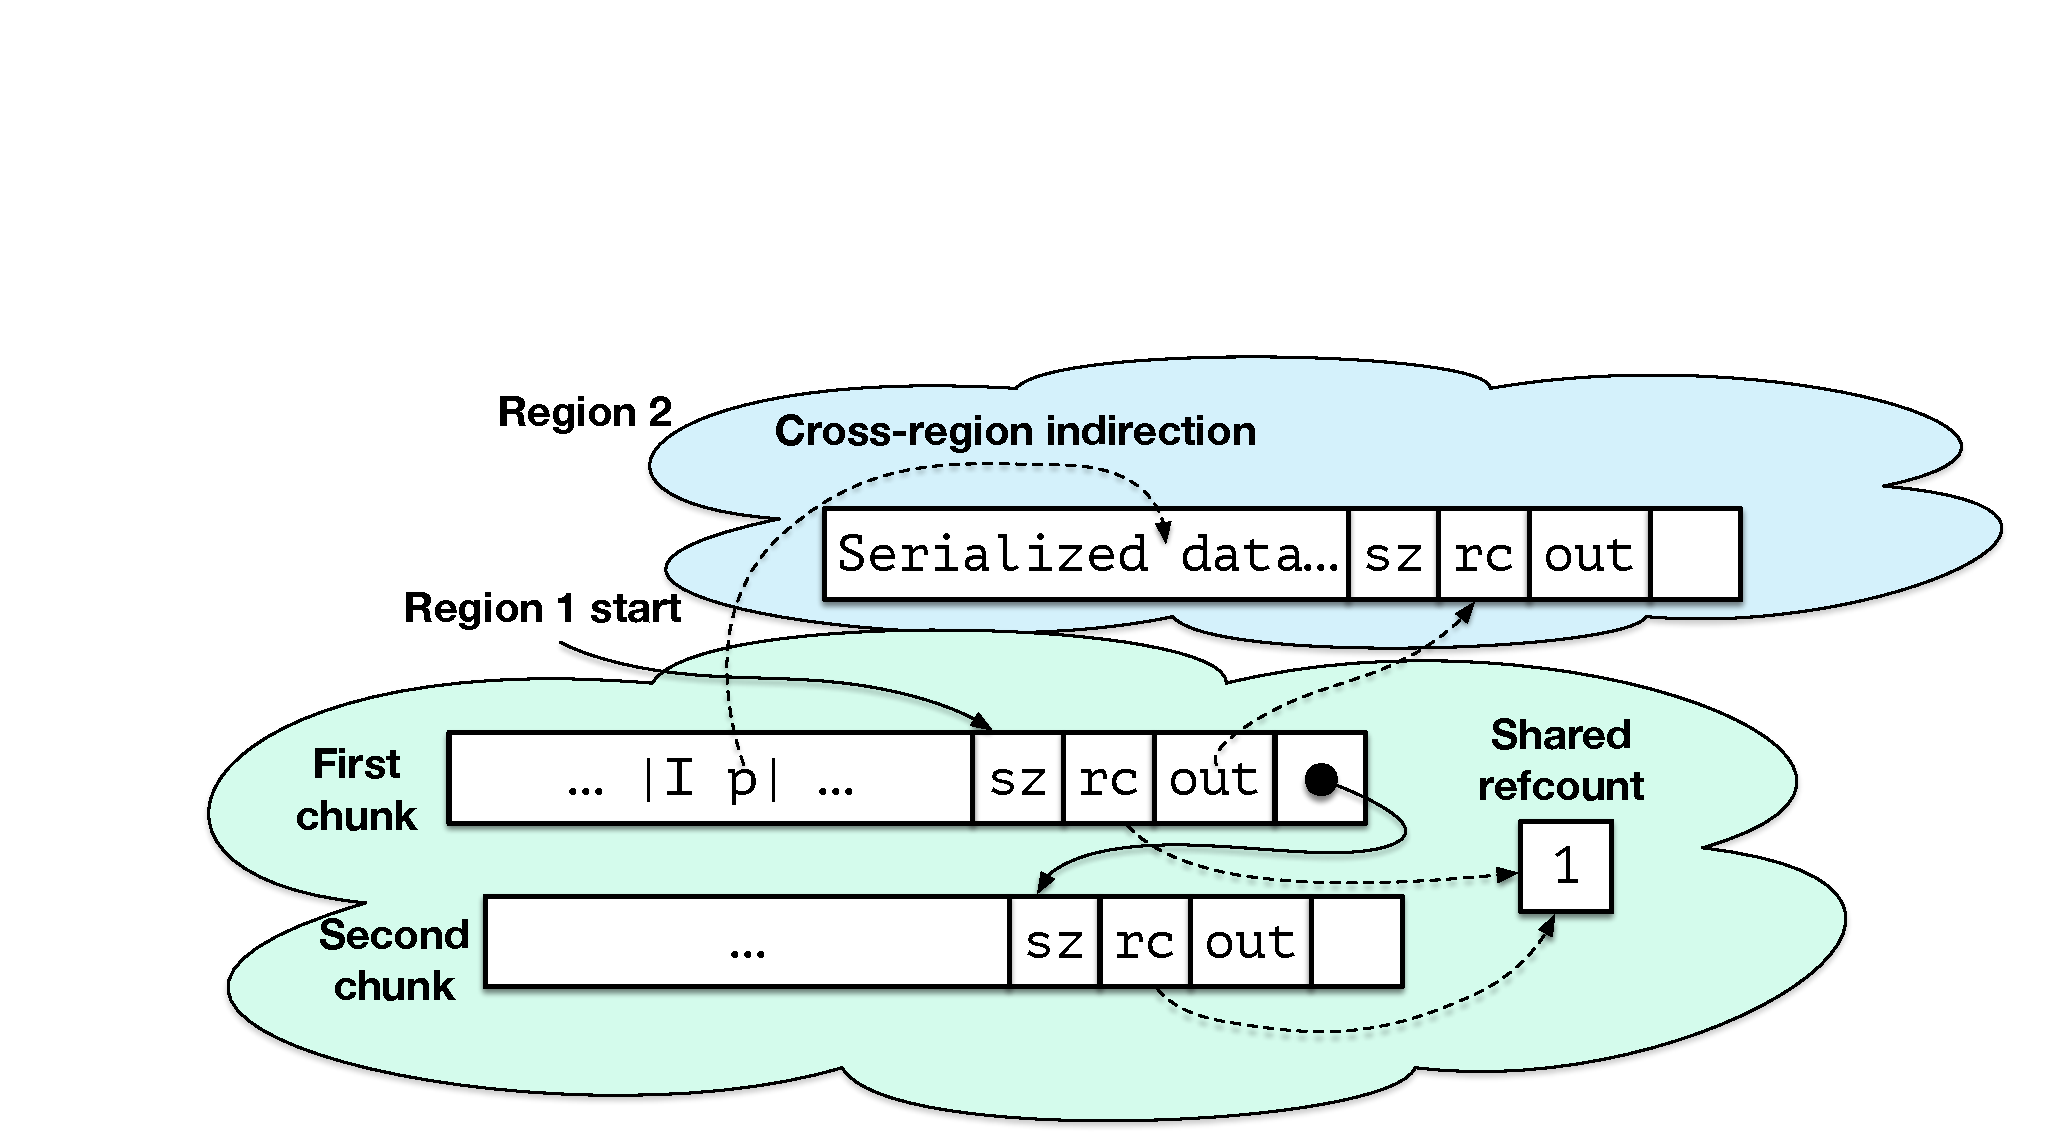
\includegraphics[width=0.75\textwidth]{region-memlayout2}
  \end{center}
  \vspace{-4mm}
  \caption{Example of multiple chunks making up a region, and of an inter-region
    indirection.  \captionscrunch{}}
  \label{fig:regions}
\end{figure}


\paragraph{Comparing against prior art's memory management}
Finally, in order to compare against other work, we also implement a technique
for {\bf huge regions}; these are allocated as a large slab containing many
pages, and could be extended by mapping new virtual memory after hitting a guard
page capping the region end.  This was the approach used by
Gibbon~\cite{ecoop17-gibbon}.
%
These huge regions avoid bounds checks when writing payloads and they are
suitable for programs with a small number of large regions (especially a single
input and single output region).  But they are inappropriate for the more
general case where programs may have small and short-lived regions.
%
%% \Red{We quantify the performance impacts of this trade-off in
%%   \secref{sec:eval-litmus}.}

%% Previous compilers based on regions, such as the MLKit compiler~\citep{mlkit},
%% can represent an extreme

The choice of allocation strategy can be informed by static information the
compiler gathers about the lifetime and potential size range of the region.  For
example, the region-based MLKit compiler achieved significant speedups from
statically classifying a majority of regions as constant-sized
\cite{mlkit-retrospective}, in which case they are allocated inside the procedure
stack frame.
%
% In our case, because we are packing many logical values into a smaller number of
In our approach, we unbox constant-sized data types (e.g. numbers), and
pack recursive data-types into growable regions, so we do not observe the same
opportunity for constant-sized regions.


%% \begin{itemize}
%% \item {\bf Bounds-check} or {\bf guard page}:
%% \item {\bf Copying} or {\bf Linking}:
%% \end{itemize}

%% The latter choice is relevant to the design of our ``mostly serialized''
%% representation, because {\em contiguity} changes the design space for
%% offset-based pointers.  For instance, if using the copying strategy


\chapter{Formalization and Type Safety Proof}

\section{Variables and Substitution}
%
We use the convention that all variables for binding values,
locations, and regions are distinct, and maintain this invariant
implicitly.
%
The bindings sites of variables are summarized by the following:
%
\begin{itemize}
\item Variables for binding values $\var$ are bound by function definitions
$\FD$ and pattern matches $\pat$.

\item Location variables $\locreg{\loc}{\reg}$ are bound by type schemes $\TS$, pattern matches
$\pat$, and $\keywd{letloc}$ binders.

\item Region variables $\reg$ are bound by type schemes $\TS$, pattern
matches $\pat$, and $\keywd{letregion}$ binders.
\end{itemize}
%
The use sites of variables are summarized by the following:
\begin{itemize}
\item Variables for binding varlues $\var$ are used by values $\VAL$.

\item Location variables $\locreg{\loc}{\reg}$ are used by concrete locations $\concreteloc{\reg}{\ind}{\locreg{\loc}{\reg}}$,
the argument list of function applications
$\fapp{\overharpoon{\locreg{l}{r}}}{\overharpoon{\VAL}}$, the location
argument of constructor applications
$\datacon{\DC}{\keywd{\locreg{\loc}{\reg}}}{\overharpoon{\VAL}}$,
located types $\hTYP$, and located expressions $\LE$.

\item Region varaibles $\reg$ are used in the same places as location variables.
\end{itemize}
%
We use the following conventions for variable substitution:
%
\begin{itemize}
\item $\subst{\EXPR}{x}{v}$: Substitute $v$ for $x$ in $e$. We let the notation extend to vectors such that
$\subst{\EXPR}{\overharpoon{x}}{\overharpoon{v}}$ denotes the iterated substitution $\subst{\EXPR}{\overharpoon{x_1}}{\overharpoon{v_1}} \ldots \subst{}{\overharpoon{x_n}}{\overharpoon{v_n}}$, where $n = |\overharpoon{x}| = |\overharpoon{v}|$.

\item $\subst{\EXPR}{\locreg{\loc_1}{\reg_1}}{\locreg{\loc_2}{\reg_2}}$: Substitute location variable $\locreg{\loc_2}{\reg_2}$ for $\locreg{\loc_1}{\reg_1}$ in $\EXPR$. We extend this notation to vectors of locations in the same fashion, as described above.

\item $\subst{\EXPR}{\reg_1}{\reg_2}$ : Substitute region variable $\reg_2$ for $\reg_1$ in $\EXPR$. We extend this notation to vectors of locations in the same fashion, as described above.

\item Finally, we extend the aforementioned notation so that
  substitution can act on environments $\CENV$, $\AENV$, and $\NENV$,
  e.g.,
  $\subst{\CENV}{\locreg{\loc_1}{\reg_1}}{\locreg{\loc_2}{\reg_2}}$.
\end{itemize}


\section{Global Environments and Metafunctions}

\begin{itemize}
\item $Function(f)$: An environment that maps a function $f$ to its definition $\FD$.

\item $Freshen(\FD)$: A metafunction that freshens all bound variables in function definition
$\FD$ and returns the resulting function definition.

\item $TypeOfCon(\DC):$ An environment that maps a data constructor to its type.

\item $TypeOfField(\DC,i)$: A metafunction that returns the type of the \il{i}'th field
of data constructor $\DC$.

\item $ArgTysOfConstructor(\DC)$: An environment that maps a data constructor to its field types.

\item $\allocptr{\reg}{\STOR}$: $\max \set{-1} \cup \set{ \indj \; | \; {(\reg \mapsto (\indj \mapsto \DC)) \in \STOR}}$.
\end{itemize}

\section{Well-formedness of the Store}
\label{sec:well-formedness}

The well formedness of the store is defined by the top-level judgement
\begin{displaymath}
\storewf{\SENV}{\CENV}{\AENV}{\NENV}{\MENV}{\STOR}
\end{displaymath}
whose definition itself uses three other judgements.
%
All of these judgements are summarized in Table~\ref{tbl:swf-judgements}.

%\floatstyle{boxed}\restylefloat{table}
\begin{table}
\bgroup
\def\arraystretch{1.2}
\setlength\tabcolsep{0.5cm}
\begin{tabular}{lclp{6cm}}
 & \textbf{Judgement form} & \textbf{Section} &\textbf{Summary}
 \\\\
\parbox[t]{3.5cm}{Store \\ well formedness} & $\storewf{\SENV}{\CENV}{\AENV}{\NENV}{\MENV}{\STOR}$ &
\ref{sec:well-formedness} &
The store $\STOR$ along with location map $\MENV$ are well formed with respect to
typing environments $\SENV$, $\CENV$, and $\AENV$.
\\\\
End witness & $\ewitness{\TYP}{\concreteloc{\reg}{\ind_{s}}{}}{\STOR}{\concreteloc{\reg}{\ind_{e}}{}}$ &
\ref{sec:end-witness} &
The store address $\concreteloc{\reg}{\ind_{e}}{}$ is the position one
after the last cell of the tree of type $\TYP$ starting at
$\concreteloc{\reg}{\ind_{s}}{}$ in store $\STOR$.
\\\\
\parbox[t]{3.5cm}{Constructor-application \\ well formedness}
 & $\storewfcfa{\CENV}{\MENV}{\STOR}$ &
\ref{sec:well-formedness-constructors} &
All in-flight data-constructor applications in store $\STOR$ along with location map $\MENV$
are well formed with respect to constructor-progress typing environment $\CENV$.
\\\\
\parbox[t]{3.5cm}{Allocation \\ well formedness} & $\storewfca{\AENV}{\NENV}{\MENV}{\STOR}$ &
\ref{sec:well-formedness-allocation} &
Allocation in store $\STOR$ along with location map $\MENV$ is well formed
with respect to allocation-typing environments $\AENV$ and $\NENV$.
\end{tabular}
\egroup
\caption{Summary of judgements used to establish well formedness of the store.}
\label{tbl:swf-judgements}
\end{table}

\paragraph{Notation for references to well-formedness judgements}
Because there are many requirements specified inside the various
well-formedness judgements, we introduce notation for referring
to requirements individually.
%
For example, the notation
\refwellformed{sec:well-formedness-allocation}{wf:impl-linear-alloc2}
refers to the judgement
\begin{align*}
\storewfca{\AENV}{\NENV}{\MENV}{\STOR},
\end{align*}
specified in Section~\ref{sec:well-formedness-allocation},
and in that judgement, rule number~\ref{wf:impl-linear-alloc2}.

The definition of store well formedness follows.

\paragraph{Judgement form}

$\storewf{\SENV}{\CENV}{\AENV}{\NENV}{\MENV}{\STOR}$

The well-formedness judgement specifies the valid layouts of the store by using the location
map and the various environments from the typing judgement.
%
Rule~\ref{wf:map-store-consistency} specifies that, for each location in the store-typing environment,
there is a corresponding concrete location in the location map and that concrete location satisfies
a corresponding end-witness judgement.
%
Rules~\ref{wf:cfc} and~\ref{wf:ca} reference the judgements for well formedness concerning
in-flight constructor applications (\secref{sec:end-witness}) and correct allocation in
regions (\secref{sec:well-formedness-allocation}), respectively.
%
Finally, Rule~\ref{wf:impl1} specifies that the nursery and store-typing environments reference
no common locations, which is a way of reflecting that each location is either in the process
of being constructed and in the nursery, or allocated and in the store-typing environment, but
never both.

\paragraph{Definition}

\begin{enumerate}

    \item \label{wf:map-store-consistency} $ (\locreg{\loc}{\reg} \mapsto \TYP) \in \SENV \Rightarrow \\
            ((\locreg{\loc}{\reg} \mapsto \concreteloc{\reg}{\ind_1}{}) \in \MENV \wedge \\
            \ewitness{\TYP}{\concreteloc{\reg}{\ind_1}{}}{\STOR}{\concreteloc{\reg}{\ind_2}{}})
          $ 

    \item \label{wf:cfc} $\storewfcfa{\CENV}{\MENV}{\STOR}$ 

    \item \label{wf:ca} $\storewfca{\AENV}{\NENV}{\MENV}{\STOR}$

    \item \label{wf:impl1} $dom(\SENV) \cap \NENV = \emptyset $
\end{enumerate}

\subsection{End-Witness judgement}
\label{sec:end-witness}

\paragraph{Judgement form}

$\ewitness{\TYP}{\concreteloc{\reg}{\ind_{s}}{}}{\STOR}{\concreteloc{\reg}{\ind_{e}}{}}$

The end-witness judgement specifies the expected layout in the store of a fully
allocated data constructor.
%
Rule~\ref{ewitness:impl1} requires that the first cell store a constructor
tag of the appropriate type.
%
Rule~\ref{ewitness:impl2} specifies the address of the cell one past the tag.
%
Rule~\ref{ewitness:impl3} recursively specifies the positions of the constructor
fields.
%
Finally, Rule~\ref{ewitness:impl4} specifies that the end witness of
the overall constructor is the address one past the end of either the
tag, if the constructor has zero fields, or the final field,
otherwise.

\paragraph{Definition}

\begin{enumerate}
\item \label{ewitness:impl1} $\STOR(\reg)(\ind_s) = \DC'$ \; \text{such that} \\
      $\; \DATA\;\TYP = \overharpoon{\DC_1 \; \overharpoon{\sTYP}_1\;} \; | \; \ldots \; | \; \DC' \; \overharpoon{\sTYP}' \; | \; \ldots \; | \; \overharpoon{\DC_m \; \overharpoon{\sTYP}_m\;}$

\item \label{ewitness:impl4} $\overharpoon{w_0} = \ind_s + 1$

\item \label{ewitness:impl2}
  $\ewitness{\overharpoon{\TYP'_1}}{\concreteloc{\reg}{\overharpoon{w_0}}{}}{\STOR}{\concreteloc{\reg}{\overharpoon{w_1}}{}} \wedge$ \\
  $\ewitness{\overharpoon{\TYP'_{j+1}}}{\concreteloc{\reg}{\overharpoon{w_j}}{}}{\STOR}{\concreteloc{\reg}{\overharpoon{w_{j+1}}}{}}$
  \\ where $\indj \in \set{1,\ldots,n-1} ; n = | \overharpoon{\TYP'} |$

\item \label{ewitness:impl3}
  $\ind_e = \overharpoon{w_n}$
\end{enumerate}

\subsection{Well-formedness of constructor application}
\label{sec:well-formedness-constructors}

\paragraph{Judgement form}

$\storewfcfa{\CENV}{\MENV}{\STOR}$

The well-formedness judgement for constructor application specifies the various constraints
that are necessary for ensuring correct formation of constructors, dealing with constructor
application being an incremental process that spans multiple \ourcalc{} instructions.
%
Rule~\ref{wfconstr:constraint-start} specifies that, if a location corresponding to the
first address in a region is in the constraint environment, then there is a corresponding
entry for that location in the location map.
%
Rule~\ref{wfconstr:constraint-tag} specifies that, if a location corresponding to the address one past a constructor
tag is in the constraint environment, then there are corresponding locations for the address
of the tag and the address after in the location map.
%
Rule~\ref{wfconstr:constraint-after} specifies that, if a location corresponding to the address
one past after a fully allocated constructor application is in the constraint environment,
then there are corresponding locations for the address one past the constructor application
and for the address of the start of that constructor application in the location map, as well as the existence
of an end witness for that fully allocated location.

\paragraph{Definition}

\begin{enumerate}
    \item \label{wfconstr:constraint-start} $ (\locreg{\loc}{\reg} \mapsto \startr{\reg}) \in \CENV \Rightarrow \\
            (\locreg{\loc}{\reg} \mapsto \concreteloc{\reg}{0}{}) \in \MENV $

    \item \label{wfconstr:constraint-tag} $ (\locreg{\loc}{\reg} \mapsto (\locreg{\loc'}{\reg} + 1)) \in \CENV \Rightarrow
            \\
            (\locreg{\loc'}{\reg} \mapsto \concreteloc{\reg}{\ind_l}{})  \in \MENV \wedge \\
            (\locreg{\loc}{\reg} \mapsto \concreteloc{\reg}{\ind_l + 1}{})  \in \MENV
            $

    \item \label{wfconstr:constraint-after} $ (\locreg{\loc}{\reg} \mapsto \afterl{\tyatlocreg{\TYP}{\locreg{\loc'}{\reg}}{\reg}}) \in \CENV \Rightarrow \\
            ((\locreg{\loc'}{\reg} \mapsto \concreteloc{\reg}{\ind_1}{}) \in \MENV \wedge \\
            \ewitness{\TYP}{\concreteloc{\reg}{\ind_1}{}}{\STOR}{\concreteloc{\reg}{\ind_2}{}} \wedge \\
            (\locreg{\loc}{\reg} \mapsto \concreteloc{\reg}{\ind_2}{}) \in \MENV)
            $

\end{enumerate}

\subsection{Well-formedness concerning allocation}
\label{sec:well-formedness-allocation}

\paragraph{Judgement form}

$\storewfca{\AENV}{\NENV}{\MENV}{\STOR}$

The well-formedness judgement for safe allocation specifies the various properties
of the location map and store that enable continued safe allocation, avoiding in particular
overwriting cells, which could, if possible, invalidate overall type safety.
%
Rule~\ref{wf:impl-linear-alloc} requires that, if a location is in both the allocation
and nursery environments, i.e., that address represents an in-flight
constructor application, then there is a corresponding location in the location
map and the address of that location is the highest address in the store.
%
Rule~\ref{wf:impl-linear-alloc2} requires that, if there is an address in the allocation
environment and that address is fully allocated, then the address of that location is the
highest address in the store.
%
Rule~\ref{wf:impl-write-once} requires that, if there is an address in the nursery, then
there is a corresponding location in the location map, but nothing at the corresponding
address in the store.
%
Finally, Rule~\ref{wf:impl-empty-region} requires that, if there is a region that has been
created but for which nothing has yet been allocated, then there can be no addresses
for that region in the store.

\paragraph{Definition}

\begin{enumerate}
    \item \label{wf:impl-linear-alloc} $ ((\reg \mapsto \locreg{\loc}{\reg}) \in \AENV \wedge \locreg{\loc}{\reg} \in \NENV) \Rightarrow \\
          ((\locreg{\loc}{\reg} \mapsto \concreteloc{\reg}{\ind}{}) \in \MENV \wedge
%          \ind = \max \set{0} \cup \set{\indj \; | \; \concreteloc{\reg}{\indj}{} \in \MENV} \wedge \\
          \ind > \allocptr{\reg}{\STOR})
          $

    \item \label{wf:impl-linear-alloc2} $ ((\reg \mapsto \locreg{\loc}{\reg}) \in \AENV \wedge 
    \, (\locreg{\loc}{\reg} \mapsto \concreteloc{\reg}{\ind_s}{}) \in \MENV \wedge \locreg{\loc}{\reg} \not \in \NENV \wedge
    \, \ewitness{\TYP}{\concreteloc{\reg}{\ind_s}{}}{\STOR}{\concreteloc{\reg}{\ind_e}{}}) \Rightarrow \\
          \ind_e > \allocptr{\reg}{\STOR}
          $

    \item \label{wf:impl-write-once} $ \locreg{\loc}{\reg} \in \NENV \Rightarrow \\
          ((\locreg{\loc}{\reg} \mapsto \concreteloc{\reg}{\ind}{}) \in \MENV \wedge \\
          (\reg \mapsto (\ind \mapsto \DC)) \not \in \STOR)
          $

    \item \label{wf:impl-empty-region} $(\reg \mapsto \emptyset) \in \AENV \Rightarrow \\
    \reg \not \in dom(\STOR)$
\end{enumerate}





\addcontentsline{toc}{chapter}{Bibliography}

\bibliographystyle{acm}
%\include{your_bibliography_name.tex}
\bibliography{refs}

% Adds a line for your CV without a page number

%% \addtocontents{toc}{%
%%   \protect\contentsline{chapter}{Curriculum Vitae}{}}
\end{document}
